\documentclass[a4paper]{article}
% ==== Inputs and Usepackages ====

\usepackage{tablefootnote}
\usepackage{enumerate}
\usepackage{float}
\usepackage{url}
\usepackage{hyperref}
\usepackage{dsfont}
\usepackage{mathrsfs}
\usepackage{amsmath}
\usepackage{amssymb}
\usepackage{amsthm}
\usepackage{amsfonts}
\usepackage{mathtools}
%\usepackage{mathabx}
\usepackage{MnSymbol}
\usepackage{xfrac}
\usepackage{nicefrac}
\usepackage{geometry}
\usepackage{graphicx}
\usepackage{graphics}
\usepackage{latexsym}
\usepackage{setspace}
\usepackage{tikz-cd}
\usepackage{tikz}
 \usetikzlibrary{matrix}
 \usetikzlibrary{calc}
 \usetikzlibrary{circuits.ee.IEC}
\usepackage{circuitikz}

\usepackage{a4wide}
\usepackage{fancybox}
\usepackage{fancyhdr}
\usepackage[utf8]{inputenc}




% ==== Page Settings ====

\hoffset = -1.2 in
\voffset = -0.3 in
\textwidth = 590pt
\textheight = 770pt
\setlength{\headheight}{20pt}
\setlength{\headwidth}{590pt}
\marginparwidth = 0 pt
\topmargin = -0.75 in
\setlength{\parindent}{0cm}


% ==== Presettings for files ====

\pagestyle{fancy}


\cfoot{\thepage}
\lfoot{\href{mailto:szekerb@student.ethz.ch}{szekerb@student.ethz.ch}}
\rfoot{Balázs Szekér, \today}
\lhead{Physics \uproman{3} Summary}


\makeatletter
\renewcommand{\maketitle}{%
  \begin{titlepage}
    \begin{center}
      \vspace*{5cm} % Adjust vertical space from top
      {\Huge\@title\par} % Title size
      \vspace{0cm} % Adjust vertical space between title and author
      {\large
        \lineskip 0.75em % Adjust line spacing here
        \begin{tabular}[t]{c}
          \@author \\
          \@date
        \end{tabular}\par}
      \vspace{1cm} % Adjust vertical space between author/date and bottom
    \end{center}
  \end{titlepage}
}
\makeatother

\title{Big Data for Engineers}
\author{\\ Summary \\ \\ \\ Balázs Szekér \\ \href{mailto:szekerb@ethz.ch}{szekerb@ethz.ch} \\ \\ Summary of the Lecture Big Data for Engineers \\ held in the Spring Semester 2024 by
Ghislain Fourny \\ \\ Swiss Federal Institute of Technology, ETH Zürich \\} 


\begin{document}
\begin{titlepage}
    \maketitle
    \thispagestyle{empty}
\end{titlepage}
\pagebreak
\pagenumbering{Roman} 
\thispagestyle{myplain}
\begin{abstract}
    This is a summary of the topics dealt with in the lecture \textit{Big Data for Engineers} in the spring semester 2024 given by Ghislain Fourny at ETH Zürich. Everything that is being mentioned in this script originates either from the lectures and lecture notes, or from the script.\footnote[1]{\url{https://ghislainfourny.github.io/big-data-textbook/}}\footnote[2]{\url{https://www.researchgate.net/publication/361334530_The_Big_Data_Textbook_-_teaching_large-scale_databases_in_universities}} The list of topics in this summary is not exhaustive. Many things were left out and only the topics which the author regarded as important are mentioned. This summary should neither be considered as a replacement of the lecture nor as a sufficient preparation for the exam. This summary should only be a reminder to which you can resort in case you quickly want to look something up. No liability is accepted in the event of failure to pass the examination.

    \vspace{1\baselineskip}

    If you stumble over mistakes, be it linguistic or thematic, or if you have suggestions what to add or how to improve this script, do not hesitate to contact me at
    \href{mailto:szekerb@ethz.ch}{szekerb@ethz.ch}.

    \vspace{1\baselineskip}

    Many Thanks
    
    \vspace{1\baselineskip}

    Balázs Szekér
\end{abstract}
\newpage
\thispagestyle{myplain}
\tableofcontents
\pagebreak
\pagenumbering{arabic}

\textcolor{red}{The only languages in which we need to code in the exam are: PostgreSQL,SQL,PySpark,SparkSQL and JSONiQ. The rest will be theoretical questions. However, in these theoretical questions, questions about other languages may appear.}

\section{Introduction}

\subsection{The three Vs of Data Science}

The three Vs of Data Science are \textit{Volume, Variety} and \textit{Velocity}.

\subsubsection{Volume}

\begin{table}[h]
    \centering
    \begin{tabular}[h]{|c|c|}
        \hline
        kilo (k) & $1'000 = 10^3$ \\ \hline
        Mega (M) & $1'000'000 = 10^6$ \\ \hline
        Giga (G) & $1'000'000'000 = 10^9$ \\ \hline
        Tera (T) & $1'000'000'000'000 = 10^{12}$ \\ \hline
        Peta (P) & $1'000'000'000'000'000 = 10^{15}$ \\ \hline
        Exa (E) & $1'000'000'000'000'000'000 = 10^{18}$ \\ \hline
        Zetta (Z) & $1'000'000'000'000'000'000'000 = 10^{21}$ \\ \hline
        Yotta (Y) & $1'000'000'000'000'000'000'000'000 = 10^{24}$ \\ \hline
        Ronna (R) & $1'000'000'000'000'000'000'000'000'000 = 10^{27}$ \\ \hline
        Quatta (Q) & $1'000'000'000'000'000'000'000'000'000'000 = 10^{30}$ \\ \hline
    \end{tabular}
    \caption{Prefixes (Powers of 10)}\label{tab:prefixes10}
\end{table}

\begin{table}[h]
    \centering
    \begin{tabular}[h]{|c|c|}
        \hline
        kibi (ki) & $1,024 = 2^{10}$ \\ \hline
        Mebi (Mi) & $1,048,576 = 2^{20}$ \\ \hline
        Gibi (Gi) & $1,073,741,824 = 2^{30}$ \\ \hline
        Tebi (Ti) & $1,099,511,627,776 = 2^{40}$ \\ \hline
        Pebi (Pi) & $1,125,899,906,842,624 = 2^{50}$ \\ \hline
        Exbi (Ei) & $1,152,921,504,606,846,976 = 2^{60}$ \\ \hline
        Zebi (Zi) & $1,180,591,620,717,411,303,424 = 2^{70}$ \\ \hline
        Yobi (Yi) & $1,208,925,819,614,629,174,706,176 = 2^{80}$ \\ \hline
    \end{tabular}
    \caption{Prefixes (Powers of 2)}\label{tab:prefixes2}
\end{table}

\subsubsection{Variety}

There are different shapes of data. Some of them are \textit{trees, unstructured data}(text){, cubes and graphs}.


\subsubsection{Velocity}

A distortion has appeard between how much data we can store in a given volume, how fast we can read it and with which latency. Three important terms are:
\begin{itemize}
    \item Capacity: How much data can we store per unit of volume?
    \item Throughput: How many bytes can we read per unit of time?
    \item Latency: How much time do we need to wait until the bytes start arriving?
\end{itemize}
In recent times, Capacity increased by a factor of $200'000'000'000 = 2 \cdot 10^11$, Throughput by a factor of $20'000 = 2 \cdot 10^4$ and Latency by a factor of $150$.
Methods to resolve this problem include parallelization and batch processing.

\begin{definition}[Big Data]
    Big Data is a portfolio of technologies that were designed to store, manage and analyze data that is too large to fit on a single machine while accomodating for the issue of growing discrepancy between capacity, throughput and latency.
\end{definition}


\pagebreak

\section{Lessons Learned from the past}

\subsection{Data Independence}

Data independence means that the logical vew on the data is clearly separated, decoupled, from its physical storage. A relational database management system (RDBMS) exposes this logical model, together with logical building blocks for manipulating it, on top of a physical layer. A database management system stack can be viewed as a four-layer stack:
\begin{itemize}
    \item A logical query language with which the user can query data
    \item A logical model for the data
    \item A physical compute layer that processes the query on an instance of the model
    \item A physical storage layer where the data is physically stored.
\end{itemize}

\subsection{Relational Database Management Systems (RDBMS)}

\subsubsection{Formalism}

Definitions of the properties of a table can be seen in \cref{fig:table}.

\begin{figure}[h]
    \centering
    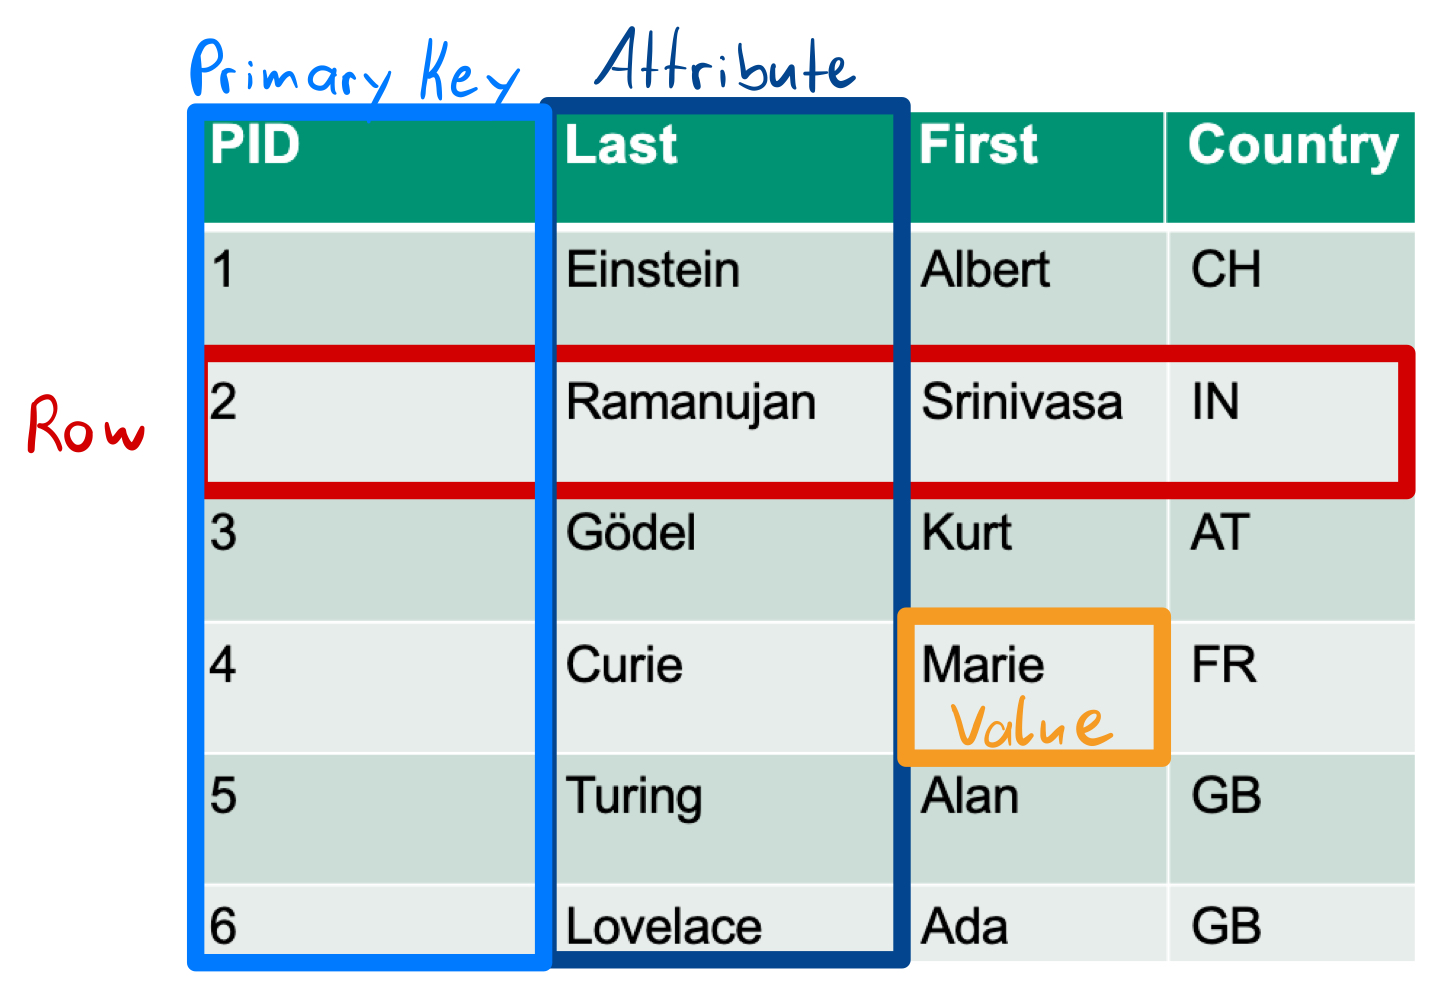
\includegraphics[width=0.7\textwidth]{Figures/Tables.jpeg}
    \caption{Table}\label{fig:table}
\end{figure}

\paragraph{Relational Integrity}
is best explained by an example such as in \cref{fig:RelInteg}.

\begin{figure}[h]
    \centering
    \begin{subfigure}{0.45\textwidth}
        \centering
        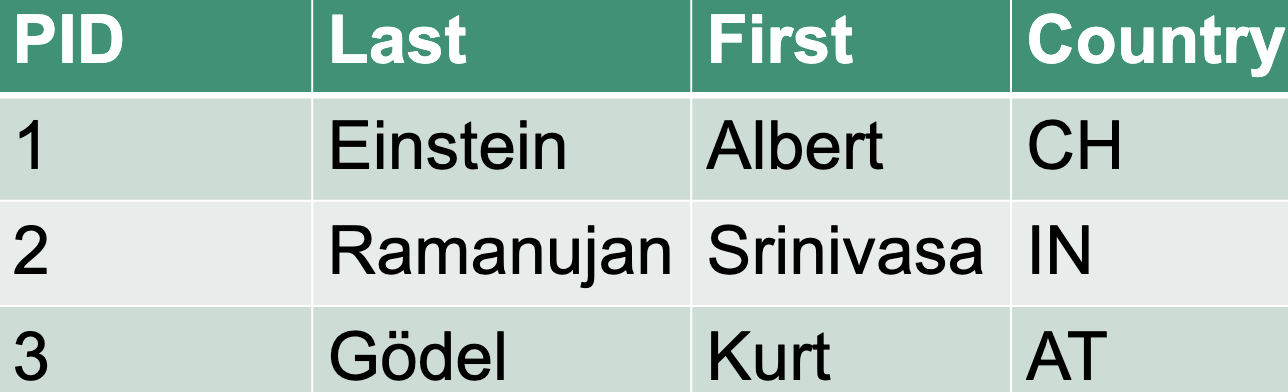
\includegraphics[width=\textwidth]{Figures/RelationalIntegrityTrue.png}
        \caption{Relational Integrity is respected.}
    \end{subfigure}
    \hfill
    \begin{subfigure}{0.5\textwidth}
        \centering
        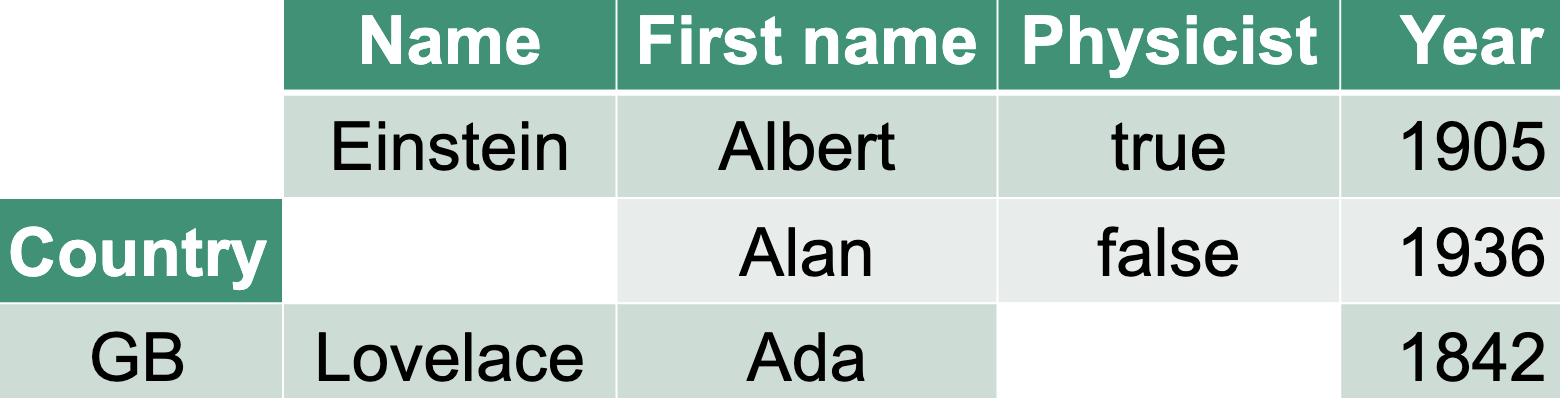
\includegraphics[width=\textwidth]{Figures/RelationalIntegrityFalse.png}
        \caption{Relational Integrity is not respected.}
    \end{subfigure}
    \caption{Examples of Relational Integrity.}\label{fig:RelInteg}
\end{figure}

\paragraph{Domain Integrity}
A table fulfills domain integrity if the values associated with each attribute are restricted to a domain. Colloquially: Each entry in an attribute column must be of the same type (character, boolean, integer,\dots).

\paragraph{Atomic Integrity}
Values in a table cannot be tables themselves. They must be atomic values.

\vspace{1\baselineskip}

The language SQL fulfills all of the three above mentioned criteria.


\subsubsection{Relational Algebra}

\paragraph{Set Queries} act on relational tables as sets. One can take the union or intersection of two sets or subtract a set from another. These operators directly and naturally translate to relational tables.

\paragraph{Filter Queries} These operators take a portion of a table: some or all columns, some or all rows, etc. They are known as projection and selection. There also exists a fancy operator called the "extended projection" that can be used to add more computed columns.

\paragraph{Renaming Queries} These operators can rename columns. Relation renaming and Attribute renaming.

\paragraph{Joining Queries} These operators can take the Cartesian product of two tables, potentially filtering to match values from both sides (join).

\paragraph{Suffling Queries} Grouping and Sorting.

\vspace{1\baselineskip}

Explanations of the previously mentioned queries:

\paragraph{Selection}
A selection takes a subset of the records belonging to the table. (A subset of the rows)

\paragraph{Projection}
A projection keeps all records, but removes columns. (A subset of the columns)

\paragraph{Grouping}
Also called aggregation, merges records by grouping on some attributes, and aggregating on all others.

\paragraph{Sorting}
Sort rows by a certain condition. E.g. alphabetic ordering of one of the attributes.

\paragraph{Cartesian Product}
A cartesian product combines each tuple from the left relational table with each tuple from the right relational table. An example can be seen in \cref{fig:CartProd}.

\begin{figure}[h!]
    \centering
    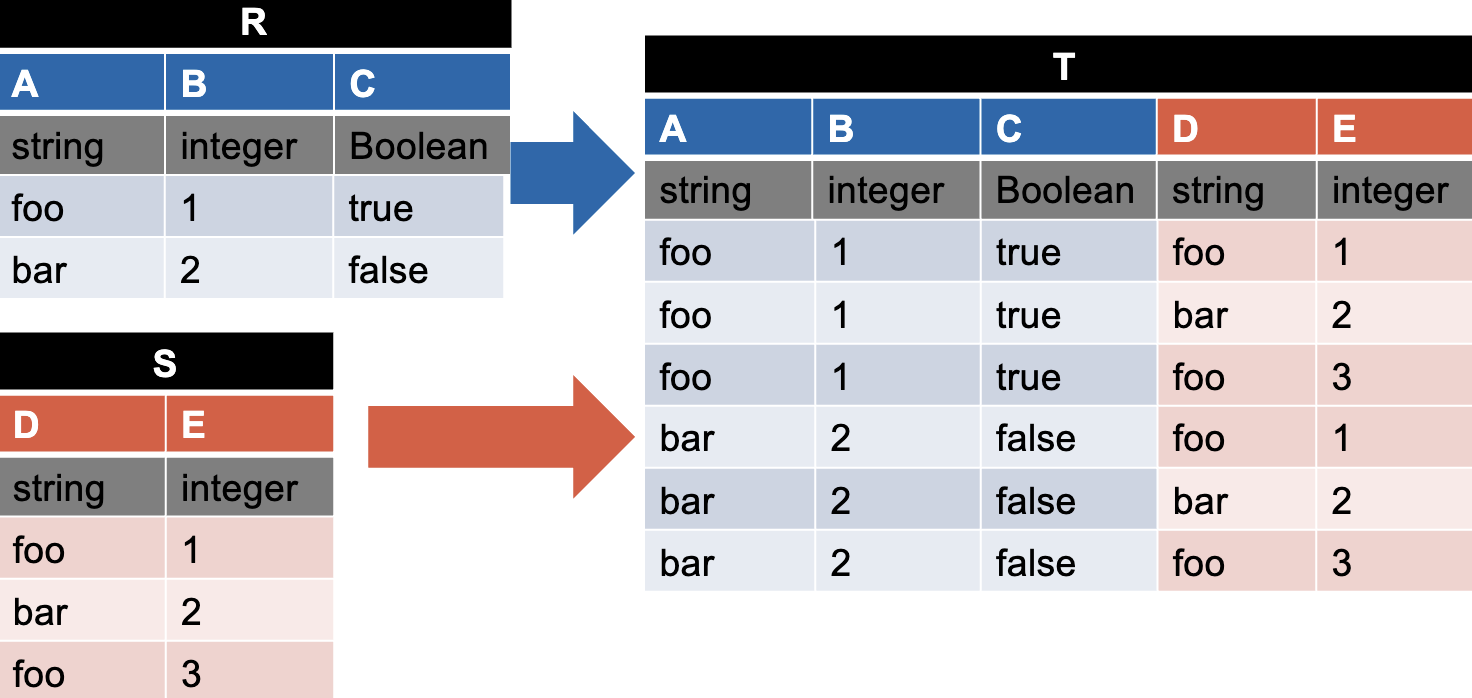
\includegraphics[width=0.7\textwidth]{Figures/CartesianProduct.png}
    \caption{Cartesian product $T = R \times S$}\label{fig:CartProd}
\end{figure}

\paragraph{Join}
A Join can be understood as a "filtered Cartesian Product" in which we only combine directly related tuples and omit all other non-matching pairs. An example can be seen in \cref{fig:Join}.
\begin{figure}[h!]
    \centering
    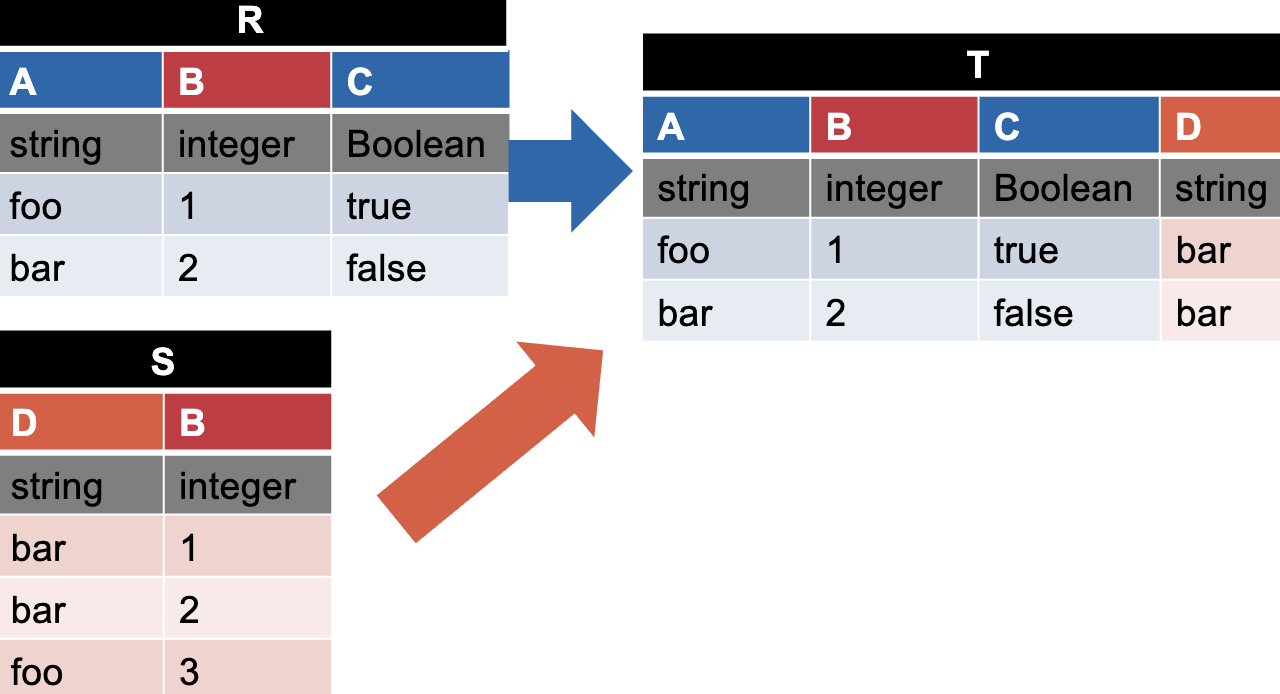
\includegraphics[width=0.7\textwidth]{Figures/Join.png}
    \caption{Join $T = R \Join S$}\label{fig:Join}
\end{figure}


\subsection{SQL}
An example that uses the most important queries can be seen in \cref{fig:SQLExmpl}.
\begin{figure}[H]
    \centering
    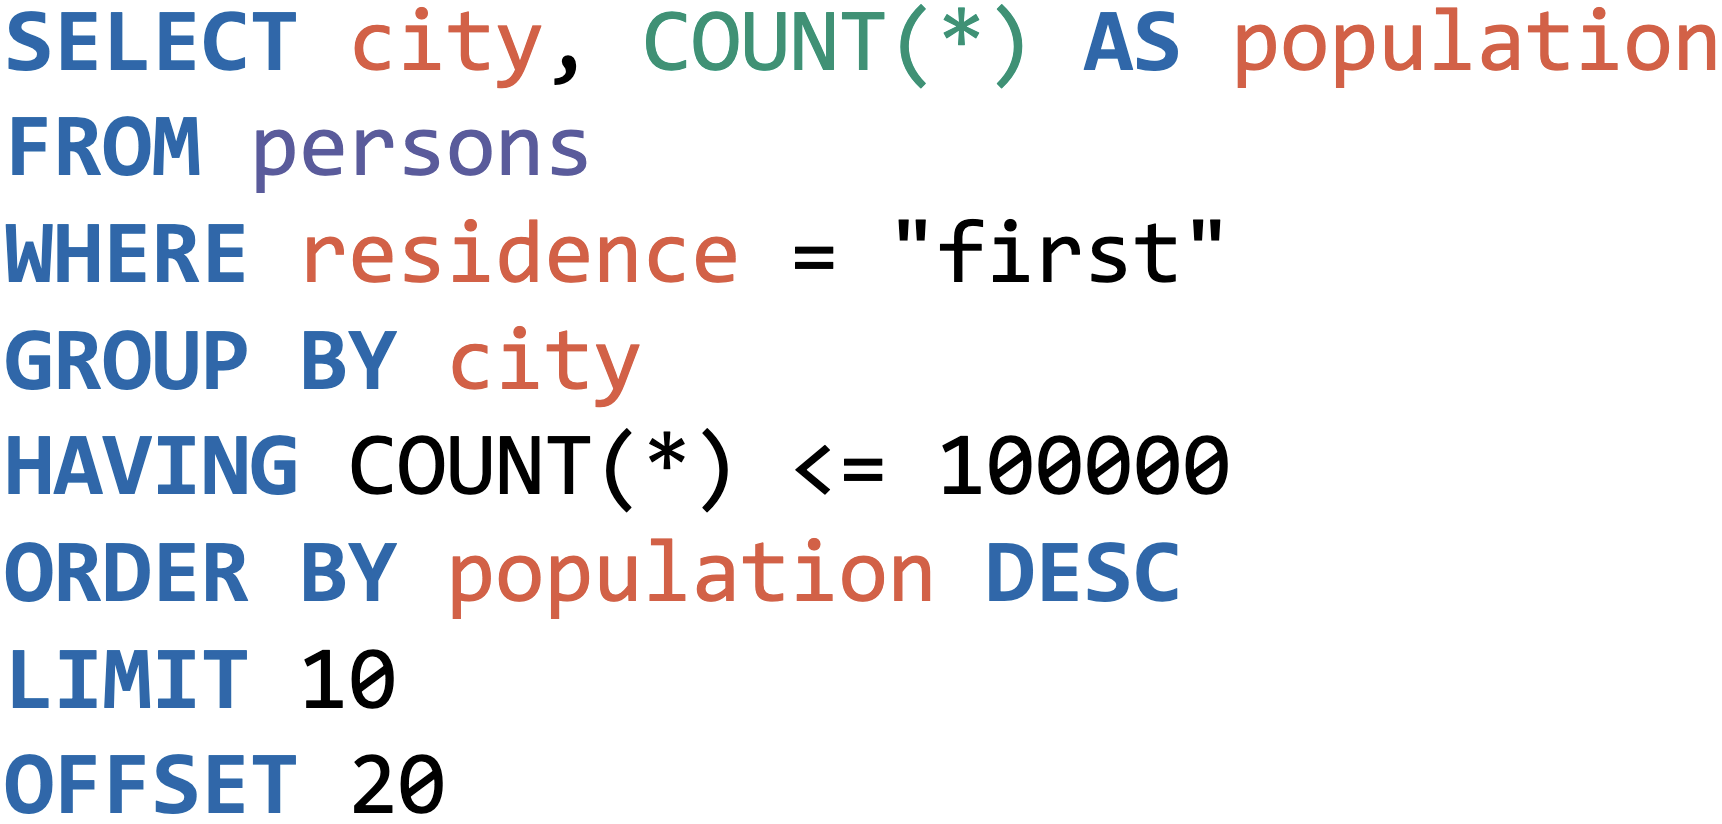
\includegraphics[width=0.5\textwidth]{Figures/ExampleSQL.png}
    \caption{Example of SQL code.}\label{fig:SQLExmpl}
\end{figure}
The SELECT clause selects which attributes of the table we want to use. We can use AS to rename certain attributes. The FROM clause selects from which tables to read the data. The WHERE clause performs a selection. The GROUP BY clause performs an aggregation. The HAVING clause is like the WHERE clause, but performs the selection after, rather than before, the grouping. The ORDER BY clause reorders the output rows according to the specified key. DESC specifies that it should be ordered in descending order. The LIMIT and OFFSET clauses allow pagination of the output: OFFSET specifies how many records (rows) to skip, and LIMIT specifies how many records (rows) to output after the skipped ones.
All clauses are optional except for SELECT and FROM.

More examples can be seen in \cref{lst:SQLExamples1}. Union queries merge two tables and duplicates are eliminated. Theta Joins are realted to normal forms. High normal form means, that we have more smaller tables. Conversely, if we have low normal forms, we have one large table with all the data. In a Theta Join, if there is match in the specified condition in the two tables, the rows are merged (one row gets more attributes). In a Full outer Join, two tables get merged just like in the Theta Join, just that all rows are added to the new table, and if there is no match in the specified condition to join, the new attributes of that row will be filled with NULL values. Natural Joins join two tables in the most natural way. No specific condition needs to be specified here.

If it is not cleare what these queries do, refer to the slides \textit{02 - Big Data - Lessons Learnt}.

\begin{lstlisting}[style=sql, caption={SQL code examples}, label={lst:SQLExamples1}]
    -- A Union Query
    SELECT * FROM TableName1 UNION SELECT * FROM TableName2;

    -- Theta Joins
    SELECT *
    FROM TableName1 JOIN TableName2
        ON TableName1.Attribute1 = TableName2.Attribute2

    -- Full outer Joins
    SELECT *
    FROM TableName1 FULL OUTER JOIN TableName2
        ON TableName1.Attribute1 = TableName2.Attribute2

    -- Natural Join
    SELECT *
    FROM TableName1 NATURAL JOIN TableName2

    -- Nesting
    SELECT attribute1, attribute2
    FROM (
        SELECT TableName1.attribute1 AS attr1,
               attribute2,
               attribute3,
               TableName2.attribute1 as attr2
               attribute 4
        FROM TableName1 FULL OUTER JOIN TableName2 USING attribute 2
    )
\end{lstlisting}

There are three-valued logics in SQL. These three values are TRUE, FALSE and UNKNOWN.

\subsection{Languages}
There are Data Manipulation Languages (DML) (e.g. query, insert, remove rows) and Data Definition Languages (DDL) (e.g. Create or table/scheme, drop it).

There are six main categories of languages: assembly code, functional and declarative languages (SQL, JSONiq, SPARQL), co-habiting with lower level APIs an. Another one are machine learning frameworks.

\paragraph{Good to know}
OnLine Transaction Processing (OLTP) is write-intensive and used if you have to modify the data a lot. Here, it is useful to use higher normal forms because you do not want to use large tables.

OnLine Analytical Processing (OLAP) is read-intensive and used for applications of Big data. Here you want to work with large dataframes. That means, we work with low normal forms.


\subsection{Transactions}
There are four main properties (ACID) that the good old systems provide:

\paragraph{Atomicity}Either an update (called a transaction if it consists of several updates) is applied to the database completely, or not at all.

\paragraph{Consistency} Before and after the transactions, the data is in a consistent state.

\paragraph{Isolation} The system "feels like" the user is the only one using (writing to) the system (databasis), where in fact maybe thousands of people are using it as well concurrently.

\paragraph{Durability} Any data written to the database is durably stored and will not be lost.


\subsection{Scaling up and out}
What happens when we have lot of rows or columns or nestings.



\pagebreak

\section{Cloud Storage}

\subsection{Storing Data}

Relational databasis management systems fit on a single machine. This is a problem if we deal with Petabytes of data, which cannot be stored on one machine.
When dealing with large amounts of data, the majority of the properties stay the same. A few things that change include:
\begin{itemize}
    \item no tabular integrity anymore
    \item no domain integrity anymore
    \item no atomic integrity anymore
    \item $2^{nd}$/$3^{rd}$/Boyce-Codd normal form are lost
    \item new heterogeneous data: data that does not fulfill domain integrity (it may not even have a schema!) and also not relational integrity.
    \item new nested data: data that is not in first normal form
    \item new denormalized data
\end{itemize}
This new domain is called NoSQL universe.

\subsection{The technology stack}
We go from a monolithic relational database to a modular "Big Data" technology stack.

\begin{figure}[h]
    \centering
    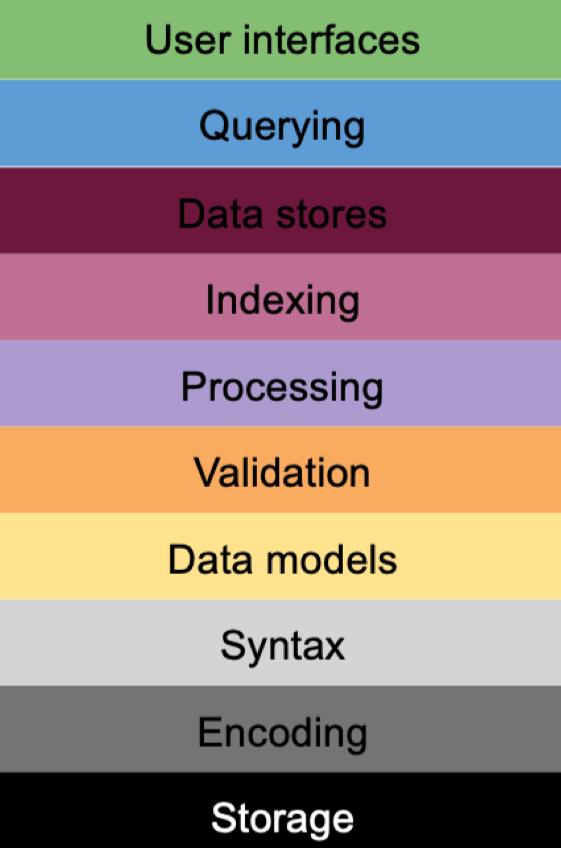
\includegraphics[width=0.35\textwidth]{Figures/Technology_Stack.jpeg}
    \caption{The Technology Stack}\label{fig:TechStack}
\end{figure}

\subsection{Databases vs. Data lakes}

In a traditional database, data can be imported into the database (this is called ETL, for Extract-Transform-Load).
In a data lake, you read directly from a file system and queried in place (in situ) by a data processing engine. This paradigm gained a lot of popularity in the past. It is slower, however users can start querying their data without the effort of ETLing.


\subsection{From your laptop to a data center}

Data are locally stored on SSDs. Files are split in blocks. This is to optimize the balance between throughput and latency.
A disk can be made available via the network (LAN for Local Area Network) and shared with other people. There exists a larger network (WAN for Wide Area Netowrks), however it is difficult to scale concurrent access and problems can arise already when two people work on a file at the same time.
Another scalability problem is that a local file system can easily support 1000 files or even 1,000,000 files, but can hardly make it to billions of files.
One approach for large scales, namely object storage, is to:
\begin{itemize}
    \item throw away the hierarchy: there are no directories
    \item make the metadata flexible: attribute can idffer from file to file (no schema)
    \item use a very simple, if not trivial, data model: a flat list of files (called objects) identified with an identifier (ID). Blocks are not exposed to the user, i.e., an object is a blackbox.
    \item use a large number of cheap machines rather than some "supercomputers"
\end{itemize}

\subsection{Scale up vs. scale out}

\paragraph{Scaling up} means, that one can buy bigger machines with more memory, more or faster CPU cores, a larger disk, etc.

\paragraph{Scaling out} means, one can buy more similar machines and share the work across them. Scaling out is much cheaper than scaling up.

\paragraph{Third way: Optimizing your code} By writing very efficient code, one can dodge having to scale out or up.

\subsubsection{Data centers}
There are tens of thousands of machines in a datacenter. The upper bound of number of machines is roughly 100,000 machines, because beyond this number, coolings starts to become critical. Furtheremore, the energy consumption is roughly the same as an airport.

There are roughly 1-200 cores per server, 1-30 TB of local storage per server, 16GB-6TB of RAM per server, 1-100 Gbits/s network bandwidth for a server.

Machines are flat and are stacked upon each other. This tower is called a \textit{Rack}.


\subsection{Object stores}

\subsubsection{Amazon S3}

It is a global cloud servive. There are buckets with bucket IDs and there are objects (files) inside the buckets (also labeled with IDs). The maximal size of a file is 5 TB and there are no buckets in buckets, and you can have a maximum of 100 buckets per user.

\paragraph{Dataset Hosting}
It may cause problems if you want to down- or upload large files to a cloud. It is therefore useful, to devide the data into chuncks and then up- or download the data chunkwise.

\paragraph{Storage Class}
There are three classes:
\begin{itemize}
    \item Standard: high availability
    \item Standard - Infrequent Access: Less availability, cheaper storage, cost for retrieving
    \item Amazon Glacier: Low-cost Hours to GET
\end{itemize}

\subsubsection{Azure Blob Storage}
Azure is also a cloud system service, with almost the same properties as Amazon S3. Some differences include:
\begin{itemize}
    \item Architecture is publicly documented
    \item Objects are identified with three instead of 2 IDs: An Account, a Container and a Blob
    \item More detail is exposed to the user. It exposes that objects are devided in several blocks more prominently than Amazon S3.
    \item It differentiates between Block Blobs, Append Blobs (for logging), and Page Blobs (for storing and accessing the memory of virtual machines).
    \item The maximum sizes are different and go from 195GB for an Append Blob to 190.7 TB for a Block Blob, and 8 TB for a page.
\end{itemize}

Azure Blob is organized in so-called storage stamps, located in various data centers worldwide. Each storage stamp consists of 10 to 20 racks, wich each rack containing around 18 storage nodes (the disk+servers). In all, a storage stamp can store up to ca. 30 PB of data. However, a storage stamp will not be filled more than 80\% of its total capacity in order to avoid being full: if a storage stamp reaches capacity, then some data is going to be reallocated to another storage stamp in the background. And if there are not enough storage stamps, well new racks will need to be purchased and installed at the location that make the most sense.

\paragraph{Storage Replication}
There are two types of storage replication.
\begin{itemize}
    \item Intra-stamp replication (synchronous): you can only work with the data if it has been stored twice or three times.
    \item Inter-stamp replication (asynchronous): communication across datacenters. You do not have to wait in this process. You can already work on other problems while the files get transfered.
\end{itemize}

\subsection{Guarantees and service level}

\subsubsection{Service Level Agreements}

Customers of cloud services one something in exchange for their money. These are:

\paragraph{Durability} The amount of information lost, each year, e.g. loss of 1 in $10^{11}$ object per year corresponds to a durability of $99.999999999\%$

\paragraph{Availability} If a service is available $99.99\%$ of the time, the server will be down less than 1h per year.

\paragraph{Response time} E.g. 99.9\% of the requests will be served in less than 300ms.


\subsubsection{The CAP theorem}

In order to scale out, many distributed systems have to make a compromise on the transactional guarantees that they offer. The CAP theorem is an impossibility triangle. A system cannot guarantee at the same time
\begin{itemize}
    \item (atomic) Consistency: at any point in time, the same request to any server returns the same result, in other words, all nodes see the same data
    \item Availability: the system is available for requests at all times (SLA with very high availability)
    \item Partition tolerance: the system continues to function even if the network linking its machines is occasionally partitioned.
\end{itemize}

\subsection{REST APIs}

REST stands for Representational State Transfer. ("HTTP done right"). A resource is refered to with a so-called URI (Uniform Resource Identifier), e.g. http://www.example.com/api/collection/foobar?id=foobar\#head where
\begin{itemize}
    \item http is the scheme
    \item //www.example.com is the authority
    \item /api/collection/foobar is the path
    \item ?id=foobar is the query
    \item \#head is the fragment
\end{itemize}
Example for Amazon S3:
http://bucket.s3.eu-west-1.amazonaws.com for a bucket and http://bucket.s3.eu-west-1.amazonaws.com/object-name for an object.

A client can act on resources by invoking methods, with an optional body. The most important methods are
\begin{itemize}
    \item GET (without a body): this method returns a representation of the resource in some format. GET should have no side effects.
    \item PUT: create or update a resource from a representation of a newer version of it, in some format. PUT has the side effect that a subsequent GET asking for the same format should return the same representation. PUT is idempotent, in that calling PUT with the same resource and body is identical to callint it just once.
    \item DELETE (without a body): this method deletes a resource. DELETE has the side effect that a subsequent GET asking for a representation of the resource should fail with a not-found (404) error.
    \item POST: this method is a blank check, in that it acts on a resource in any way the data store seems fit. The behaviour, of course, should be publicly documented. A typical use of POST is to create new resources but letting the REST server pick a resource URI for this new resource.
\end{itemize}

\subsection{Summary}

How to scale out?
Simplify the model, Buy cheap hardware, remove schemas

\pagebreak

\section{Distributed File Systems}

Big data can have different forms. You cn either have a huge amounts of large files or large amounts of huge files. I.e. Billions of TB files vs. Millions of PB files. For the first case, we use Key-Value Model and Object storage and for the second one we use File System and Block Storage.

\subsection{Main Requirements of a Distributed File System}

\paragraph{Fault tolerance and robustness} Local dist might fail, but in clusters with 100s to 10,000s of machines, the nodes will fail! Thus, storage technologies must be capable of: monitoring itself, detecting failures, automatically recovering and fault being, in the end and as a whole, fault tolerant.

\paragraph{File read and update model}
You can either have random access, meaning any part of the disk can be read and written at any time, and in any order. For distributed data storage, and for reading and writing large datasets, random access is not needed. We rather need to be able to efficiently scan a large file (in its entirety) - for data analysis, and be able to append efficiently new data at the end of an existing large file - particularly for logging sensors. We need to make sure that if one client is appending something to a file, another client cannot simultaneously add something to the file. This is called atomic.

\paragraph{Performance requirements}
Top priority: the bottleneck must be throughput. We do not want the bottleneck to be latency. Remember: the discrepancy between capacity and throughput can be resolved by parallelism and the discrepancy between throughput and latency can be resolved by batch processing.


\subsection{The Model behind HDFS}

\paragraph{File Hierarchy}
The HDFS cluster organizes its files as a hierarchy, called the file namespace. Files are thus organized in directories, similar to a local file system. (In a Key-Value Model we talk about objects, whereas in a File Hierarchy we talk about files.)

\paragraph{Blocks}
Unlike in S3, HDFS files are furthermore not stored as monolithic blackboxes, but HDFS exposes them as lists of blocks - also similar to a local file system. (Block Storage instead of Object Storage, where the whole data is saved as one big block.) The blocks are even exposed to the user. Files in an HDFS Cluster are stored as a list of blocks.

Why do we need blocks? For PB-sized files, we cannot fit the whole data on one machine (as of right now). Second, it is a level of abstraction simple enough that can be exposed on the logical level. Third, blocks can easily be spread at will across many machines.

\paragraph{The size of the blocks}
Typical sizes of blocks are 4 kB for a simple file system, 4 kB - 32 kB for a relational database and 64 MB - 128 MB for HDFS. Thsi is because of the prerequisits of HDFS: first, it is not optimized for random access, and second, blocks will be shipped over the network. 128 MB is a good sweetspot such that the blocks are large enough that the time not lost in latency, and at the same time small enough for a large file to be conveniently spread over many machines, allowing for parallel access, and also small enough for a block to be sent again without too much overhead in case of a network issue.


\subsection{Physical Architecture}
How is the cluster of machines connected? One way to connect machines is called peer-to-peer, decentralized network. In this network architecture, each machine talks to any other machine. By contrast, HDFS is implemented on a fully centralized architecture, in which one node is special and all others are interchangeable and connected to it. In HDFS we call the different nodes Namenode and Datanode.

If we want to store a file on HDFS we need to devide the data into 128 MB chunks called Block and distribute them among the datanodes. However, we also replicate them. Each block is stored three times. Each of these blocks is called a replica and they to not have a particular order. This enables to still be able to access the datablocks, eventhough a datanode might be down. Furthermore, you can also distribute the blocks among the globe, and a client can access the node closest to him or her in order to retrieve the data the fastest.

\subsubsection{The responsibilities of the NameNode}
The NameNode is responsible for the system-wide activity of the HDFS cluster. It stores in particular three things:
\begin{itemize}
    \item The File Namespace: The hierarchy of directory names and file names, as well as any access control (ACL) information similar to Unix-based systems.
    \item A mapping from each file to the list of its blocks. Each block in this list is represented with a 64-bit identifier; the content of the blocks is not on the NameNode.
    \item A mapping from each block represented with its 64-bit identifier, to the locations of its replicas, that is, the list of the DataNodes that store a copy of this block.
\end{itemize}
The NameNode updates this information whenever a client connects to it in order to update files and directories, as well as with the regular reports it receives from the DataNodes. Clients connect to the NameNode via the Client Protocol. Clients can perform metadata operations such as creating or deleting a directory, but also ask to delete a file, read a file or write a new file. In the latter case, the NameNode will send back to the client block identifiers (for reading them), or lists of DataNode locations (for reading and writing them).

\subsubsection{The responsibilities of the DataNode}
The DataNodes store the blocks themselves. These blocks are stored on their local disk.
DataNodes send regular heartbeats to the Namenode with a frequency (configurable) of a few seconds. DataNodes also send, every couple of hours, a full report including all the blocks that it contains.
If there is an issue with the local disk or the node, then the DataNode can report the block as corrupted to the NameNode, which will then ensure, asynchronously, its replication to somewhere else. "Asynchronously", as opposed to “synchronously,”, means that this is done in the background at some later time and the DataNode does not wait for this to happen.
NameNodes never connect to the DataNodes. They wait until the next heartbeat of the DataNode and answer to it with the request if there is one.

\begin{figure}[h]
    \centering
    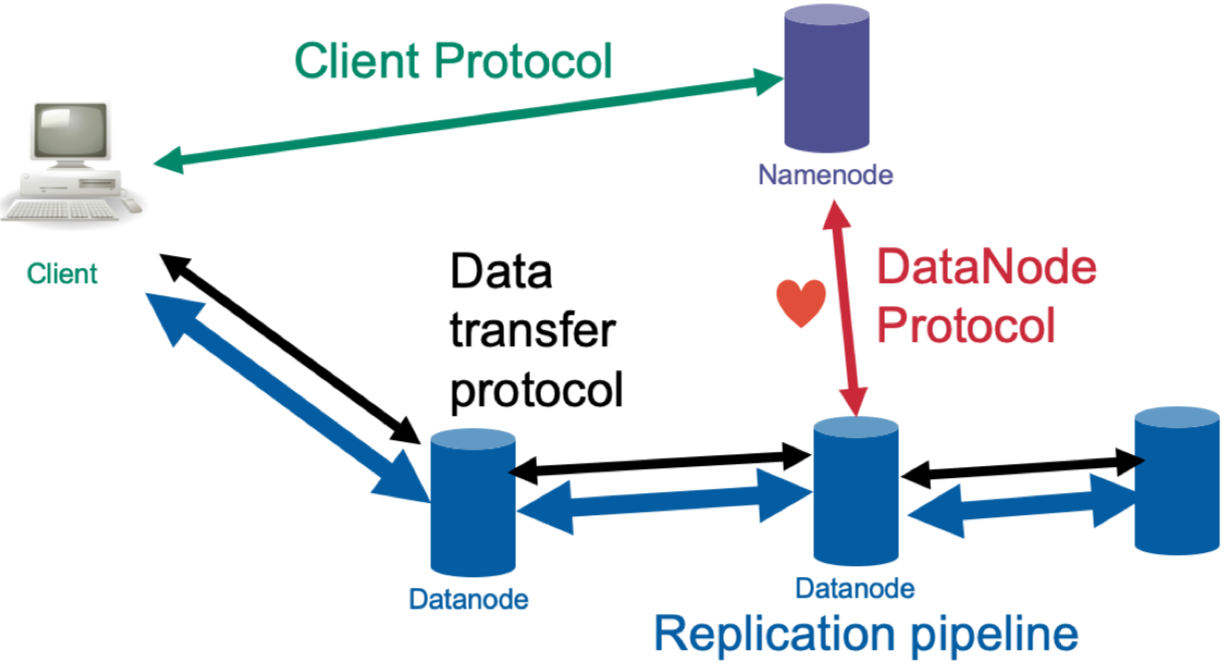
\includegraphics[width=0.7\textwidth]{Figures/ClientProtocol.png}
    \caption{Client Protocol}\label{fig:ClientProtocol}
\end{figure}

\paragraph{Client Protocol}
The NameNode is the first Node the Client will interact with.
A client can perform Metadata operations (create a directory, create a file, delete a file, etc.) and the NameNode will send back the DataNode location and Block IDs. This is all doable with a Java API.

\paragraph{DataNode Protocol}
The DataNode always initiates the connection! The DataNode sends information about the Registration, Heartbeat (every 3s), BlockReport (every 6h) and BlockReceived to the NameNode and the Name node returns Block operations.

\paragraph{Data Transfer Protocol (Streaming)}
The Client is only going to connect to the closest node, and when creating a file, the client does not need to connect to two other DataNodes to store the copy of the file, but the DataNodes will to that themselves.


\subsubsection{File System Functionality}

Metadata functionalities include \textit{Create directory, Delete directory, Write file, Append to file, Read file} and \textit{Delete file}.

\paragraph{Reading a File}
First, the client needs to connect to the NameNode to initiate the read and request info on the file. Then, the NameNode responds with the list of all blocks, as well as a list of DataNodes that contains a replica of each block. The DataNodes are furthermore sorted by increasing distance of the client (which is typically itself one of the nodes in the cluster, we will come back to this). The client then connects to the DataNodes in order to download a copy of the blocks. It starts with the first (closest) DataNode in the list provided by the NameNode for each blocks, and will go down the list if a DataNode cannot be reached or is not available. In the simple case that the client wants to stream its way through an HDFS file, bit by bit, it will download each block in turn. Note that with streaming, it is possible to process files larger than the working memory, because older blocks can be thrown away from the memory of the client once processed.

\paragraph{Write a file}
The client first conneects to the NameNode formulating its intent to create a new file. The NameNode will respond with the Block ID and a list of DataNodes to which the content of the first block should be sent. At that point the file is not yet guaranteed to be available for read for other clients, and it is locked in such a way that nobody else can write to it at the same time. The client then connects to the first DataNode and instructs it to organize a pipeline with the other DataNodes provided by the NameNode for this block. The client then starts sending through the content of that block, as we explained earlier. The content will be pipelined all the way to the other DataNodes. The client receives regular acknowledgements from the first DataN- ode that the bits have been received. When all bits have been acknowledged, the client connects to the NameNode in order to move over to the second block. Then, the same steps (2, 3, 4, 5) as before are repeated for each block. Once the last block has been written, the client informs the Na- meNode that the file is complete, and asks to release the lock. The NameNode then checks for minimal replication through the DataNode protocol and gives its final acknowledgement to the client. From now on, and separately (this is called “asynchronous”), the NameNode will continue to monitor the replicas and trigger copies from DataNode to DataNode whenever necessary, that is, when a block is underreplicated.

\subsection{Replication Strategy}
There is no order for the replicas and there usually are three replicas. How is it decided where the copies are stored? We need to consider reliability, Read/Write Bandwidth and Block distribution. One can define a distance between two nodes. The distance is defined as the "number of connecting lines between two nodes". If two nodes are in the same rack, the distance is equal to two (one from node A to the Rack, and one from the rack to node B). If two nodes are in diferent racks but still in the same cluster, then the distance is 4 (node A $\rightarrow$ Rack 1 $\rightarrow$ Cluster $\rightarrow$ Rack 2 $\rightarrow$ Node B). There are some rules where to store the replicas.
\begin{itemize}
    \item Replica 1: Same node as client (or random), rack A
    \item Replica 2: a node in a different rack B
    \item Replica 3: a node in same rack B
    \item Replica 4 and beyond: random, but if possible:
        \begin{itemize}
            \item at most one replica per node
            \item at most two replicas per rack
        \end{itemize}
\end{itemize}

\subsection{Fault Tolerance and Availability}
HDFS has a single point of failure: the NameNode. If the metadata stored on it is lost, then all the data on the cluster is lost, because it is not possible to reassemble the blocks into files any more. For this reason the metadata is backed up. More precisely, the file namespace containing the directory and file hierarchy as well as the mapping from files to block IDs is backed up to a so-called snapshot. Note that the mapping of block IDs to DataNodes does not require a backup, as it can be recovered from the periodic block reports (heartbeats). Since the HDFS system is constantly updated, it would not be viable to do a backup upon each update. It would also not be viable to do backups less often, as this could lead to data loss. Thus, what is done is that updates to the file system arriving after the snapshot has been made are instead stored in a journal, called edit log, that lists the updates sorted by time of arrival. The snapshot and edit log are stored either locally or on a network- attached drive (not HDFS itself). For more resilience, they can also be copied over to more backup locations. If the NameNode crashes, it can be restarted, the snapshot can be loaded back into memory to get the file namespace and the mapping of the files to block IDs. Then the edit log can be replayed in order to apply the latest changes. And the NameNode can wait for (or trigger) block reports to rebuild the mapping from block IDs to the DataNodes that have a replica of them.

It can take roughly 30 minutes to restart the NameNode after a crash. If in the meantime more clients make changes on some nodes, the log will not be updated while the NameNode si reset. Thus, a new stragegy hat to be put in place.

First, the edit log is periodically merged back into a new, larger snapshot and reset to an empty edit log. This is called a checkpoint. This can be done with a “phantom NameNode” (our terminology) that keeps the exact same structures in its memory as the real NameNode, and performs checkpoints periodically.

Second, it is possible to configure a phantom NameNode to be able to instantly take over from the NameNode in case of a crash. This considerably shortens the amount of time to recover. This is called a Standby NameNode.

Third, there are so-called observer NameNodes. It is similar to the Standby NameNode, but does not just stand in the shadow, it is also allowed to deliver read requests.

Fourth, there are so-called Federated NameNodes. In this change, several NameNodes can run at the same time, and each NameNode is responsible for specific (non overlapping) directories within the hierarchy. This spreads the management workload over multiple nodes.


\subsection{Using HDFS}

\begin{lstlisting}[style=hdfs, caption={Example HDFS code}, label={lst:hdfs}]
// HDFS commands start with
hdfs dfs <put command here>
// or (better)
hadoop fs <put command here>
// List the contents of the current directory with:
hadoop fs -ls
// Print to screen the contents of a file with:
hadoop fs -cat /user/hadoop/dir/file.json
// Delete a file with:
hadoop fs -rm /user/hadoop/dir/file.json
// You can create a directory with:
hadoop fs -mkdir /user/hadoop/dir/file.json
// You can upload files from your local computer to HDFS with:
hadoop fs -copyFromLocal localfile1 localfile2 /user/hadoop/targetdirectory
// You can upload a file from HDFS to your local computer with:
hadoop fs -copyToLocal /user/hadoop/file.json localfile.json
\end{lstlisting}



\pagebreak

\section{Syntax}

\subsection{Why Syntax?}

We want to be able to express text or characters in general as 0s and 1s. There are several ways for doing this. These include ASCII, ISO Latin 1, UTF-8 and UTF-16.

\subsubsection{CSV}
CSV stands for comma separated values and is a text representation of tables. On the first line you typically have the headers and on every row you have one record. The problem with CSV is that there are different conventions. Some people use another character than a comma to separate the columns, which limits interoperability. Furthermore, you might need to use certain characters in your table, such as commas, thus you need to find another symbol to use as a separator between columns. If you need a comma in one cell of your tabel, make "quotation marks" around that cell entry. If you need "quotation marks" in your cell, use """tripple quotation"" marks" in your cell.

\subsubsection{Data Denormalization}
As a rule of thumb, normalizing data means joining it back at query time. For data lakes and large-scale data processing, it is often desirable to go exactly the opposite way, called data denormalization. In this case, we can nest data. Data denormalization makes a lot of sense in read-intensive scenarios in which not having to join brings a significant performance improvement. In write-intensive cases, high normal forms make more sense because we want to avoid update anomalies.

A new tool we use for tables that are not in normal form is JSON. A tuple, mathematically a partial mapping function, can be expressed as follows (\cref{lst:json1}). Furthermore, one is also allowed to break relational integrity.

\begin{lstlisting}[style=json, caption={Example JSON code}, label={lst:json1}]
{
    "key": "value",
    "array": [1, 2, 3],
    "nested": {
        "nested_key": "nested_value",
        "nested_table": [
            {"Customer": "John", "quantity": "one"},
            {"Customer": "Peter", "quantity": 2},
            {"Customer": "John"}
        ]
    }
}
\end{lstlisting}

\subsection{Semi-Structured Data and Well-Formedness}
The generic name for denormalized data (in the same of heterogeneous and nested) is “semi-structured data”. Textual formats such as XML and JSON have the advantage that they can both be processed by computers, and can also be read, written and edited by humans. Another very important and characterizing aspect of XML and JSON is that they are standards: XML is a W3C standard. W3C, also known as the World Wide Web consortium, is the same body that also standardizes HTML, HTTP, etc. JSON is now an ECMA stan- dard, which is the same body that also standardizes JavaScript.

When a document is well-formed XML(/JSON), it means that it can be successfully opened by an editor as XML(/JSON) with no errors. On the other hand, a non-well-formed document cannot be used and cannot benefit from all the XML and JSON tools until it is fixed and edited into a well-formed document.

\subsection{JSON}
JSON is made of exactly six building blocks: strings, numbers, Booleans, null, objects, and arrays. Let us go through them.

\subsubsection{Strings}
Strings are simply text. In JSON, strings always appear in double quotes. Obviously, strings could contain quotes and in order not to con- fuse them with the surrounding quotes, they need to be differentiated. This is called escaping and, in JSON, escaping is done with backslash characters ($\backslash$). Other escape sequences include:
\begin{itemize}
    \item $\backslash \backslash$ : $\backslash$
    \item $\backslash$n : new line
    \item $\backslash$r : carriage return
    \item $\backslash$t : tabulation
    \item $\backslash$u followed by four hexadecimal digits : any character (via its Unicode code point)
\end{itemize}

\subsubsection{Numbers}
The way a number appears in syntax is called a lexical representation, or a literal. There are only a few restriction: a leading + is not allowed, a leading 0 is not allowed (with the exception of decimals). In JSON, numbers are unquoted.

\subsubsection{Booleans}
There are two Booleans, true and false, and each one is associated with exactly one possible literal, which are, well, true and false. Booleans are also unquoted.

\subsubsection{Null}
There is a special value, null, which corresponds to the (unique) literal. Some like to see this as an unknown or hidden value, others as equivalent to an absent value, etc. In this course, on the logical level, we will consider that an absent value is not the same thing as a null value.
Null literals are unquoted. Otherwise, they would be recognized as strings by the parser and not as nulls.

\subsubsection{Arrays}
Arrays are simply lists of values. The members of an array can be any JSON value: string, number, Boolean, null, array, or object. They are listed within square brackets, and are separated by commas.
\begin{lstlisting}[style=json, caption={Examples of Arrays}, label={lst:json2}]
[1,2,3]
[ ]
[null,"foo",12.3,false,[1,3]]
\end{lstlisting}

\subsubsection{Objects}
Objects are simply maps from strings to values. The keys of an object must be strings and thus must be quoted. The values associated with them can be any JSON value: string, number, Boolean, null, array, or object. The pairs are listed within curly brackets, and are separated by commas. Within a pair, the value is separated from the key with a colon character. The JSON standard recommends for keys to be unique within an object.
\begin{lstlisting}[style=json, caption={Examples of Objects}, label={lst:json2}]
{ "foo" : 1 }
{}
{ "foo" : "foo", "bar" : [ 1, 2 ],
  "foobar":[{"foo":null}, {"foo":true}]
}   
\end{lstlisting}


\subsection{XML}
XML stands for eXtensible Markup Language. It resembles HTML, except that it allows for any tags and that it is stricter in what it allows. XML is considerably more complex than JSON but, fortunately, most datasets only use a subset of what XML can do. In our course, we will stick to the most common features of XML. XML’s most important building blocks are elements, attributes, text and comments.

\subsubsection{Elements}
XML is a markup language, which means that content is “tagged”. Tagging is done with XML elements. An XML element consists of an opening tag, and a closing tag. What is “tagged” is everything inbetween the opening tag and the closing tag.

\begin{lstlisting}[style=xml, caption={Example XML code}, label={lst:xml1}]
<person>(any content here)</person>
<!-- If there is no content at all, we can write empty elements with a simple tag -->
<person/>
<!-- which is equivalent to -->
<person></person>
<!-- Elements nest arbitrarily -->
<person><first>(some content)</first><student/>
<last>(some other content)</last></person>
<!-- It is possible to use indentation and new lines to pretty- print the document for ease of read by a human: -->
<person>
  <first>(some content)</first>
  <student/>
  <last>(some other content)</last>
</person>
c
<persons>
  <person>
    <first>(some content)</first>
    <last>(some other content)</last>
  </person>
  <person>
    <first>(some content)</first>
    <last>(some other content)</last>
  </person>
  <person>
    <first>(some content)</first>
    <last>(some other content)</last>
  </person>
</persons>
\end{lstlisting}
Inner elements must be closed before the outer elements. A well-formed XML document must have exactly one element.

\subsubsection{Attributes}
Attributes are key-value pairs. Attributes can be double quoted or single quoted. The key is never quoted and there cannot be duplicate keys. Attributes can also appear in empty element tags, but cannot appear in a closing tag. Furthermore, elements canno tnest within attribute values. And lastly, attributes are not allowed to start with XML or xml or any combinatino.

\begin{lstlisting}[style=xml, caption={Example XML code}, label={lst:xml2}]
<person birth="1879" death='1955'>
    <first>(some content)</first>
    <last>(some other content)</last>
</person>
\end{lstlisting}

\subsubsection{Text}
Text is freely appearing in elements and without any quotes (attribute values are not text!). E.g.
\begin{lstlisting}[style=xml, caption={Example XML code}, label={lst:xml3}]
<person birth="1879" death="1955">
    <first>Albert</first>
    <last>Einstein</last>
</person>
<!-- Text cannot appear on its own at the top level. This is wrong: -->
Albert <person/> Einstein
<!-- Within an element, text can freely alternate with other elements, called mixed content. This is unique to XML -->
<person>
    <style>His Royal Highness</style>
    The <title>Duke of <location>Cambridge</location></title>
</person>
\end{lstlisting}

\subsubsection{Comments}
Examples of comments have been seen in the previous example blocks. However, a single comment is not well-formed XML (remember: we need exactly one top-level element). Comments can also appear at the top-level though, but under the condition that there is exactly one top-level element.
\begin{lstlisting}[style=xml, caption={Example XML code}, label={lst:xml4}]
<person birth="1879" death="1955">
    <first>Albert</first>
    <last>Einstein</last>
    <!-- He is still famous today -->
</person>
\end{lstlisting}

\subsubsection{Text declaration}
XML documents can be identified as such with an optional text decla- ration containing a version number and an encoding.
\begin{lstlisting}[style=xml, caption={Example XML code}, label={lst:xml5}]
<?xml version="1.0" encoding="UTF-8"?>
<person birth="1879" death="1955">
    <first>Albert</first>
    <last>Einstein</last>
</person>
\end{lstlisting}
Another tag that might appear right below, or instead of, the text declaration is the doctype declaration. It must then repeat the name of the top-level element, like so:
\begin{lstlisting}[style=xml, caption={Example XML code}, label={lst:xml6}]
<?xml version="1.0" encoding="UTF-8"?>
<!DOCTYPE person>
<person birth="1879" death="1955">
    <first>Albert</first>
    <last>Einstein</last>
</person>
\end{lstlisting}

\subsubsection{Summary}

\begin{table}[H]
    \centering
    \begin{tabular}{|c|c|c|c|}
        \hline
         & Top-Level & Between Element Tags & Inside Opening Element Tag \\ \hline
        Elements & once & yes & no \\ \hline
        Attributes & no & no & yes \\ \hline
        Text & no & yes & no \\ \hline
    \end{tabular}
    \caption{What appears where?}\label{tab:Waw}
\end{table}

\subsubsection{Escaping special characters}
In XML escaping is done with an ampersand (\&) character. There are exactly five possible escape sequences pre-defined in XML:
\begin{table}[H]
    \centering
    \begin{tabular}{cc}
        \hline
        Escape sequence & Corresponding character \\ \hline
        \&lt; & $<$ \\
        \&gt; & $>$ \\
        \&quot; & " \\
        \&apos; & ' \\
        \&amp; & \& \\ \hline
    \end{tabular}
    \caption{Escape characters}\label{tab:escchar}
\end{table}
Escape sequences can be used anywhere in text, and in attribute values. At other places (element names, attribute names, inside comments), they will not be recognized or will lead to well-formedness errors.
In text, \& and $<$ must(!) be escaped. The other characters may, but need not to, be escaped. In double-quoted attribute values ",\& and $<$ must(!) be escaped. The other characters may, but need not to, be escaped. In single-quoted attribute values ',\& and $<$ must(!) be escaped. The other characters may, but need not to, be escaped.

\subsubsection{XML Names}
There are a few rules how one can name an element.
\begin{itemize}
    \item An element name may not start with a digit. (wrong: $<$1234/$>$)
    \item An element name may not contain the $<$ sign and one cannot escape it. (wrong: $<$a$<$b/$>$)
    \item An element may not be named xml (by the user, developers of the service may use it, no matter the spelling (capitalized, not capitalized, mixed capitalization)). (wrong: $<$xml/$>$)
\end{itemize}

\begin{figure}[h]
    \centering
    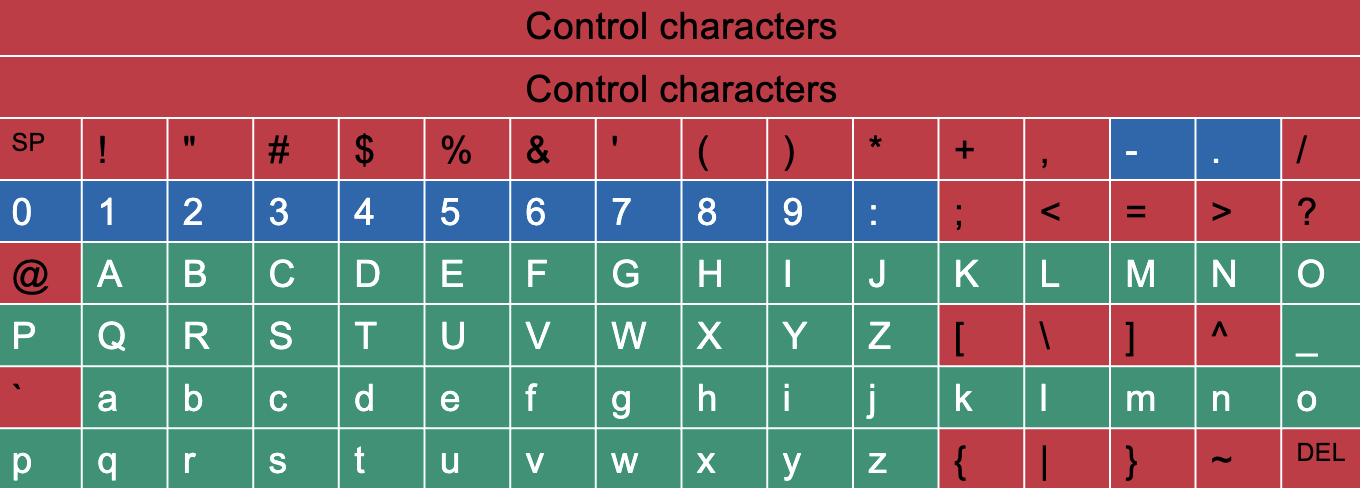
\includegraphics[width=0.7\textwidth]{Figures/CharactersAllowed.png}
    \caption{ASCII characters allowed in XML names. \textcolor{darkgreen}{Green: Allowed anywhere in name}, \textcolor{darkblue}{Blue: allowed but not at the start}, \textcolor{darkred}{Red: not allowed}.}\label{fig:charallow}
\end{figure}

\subsubsection{Namespaces in XML}

\textcolor{grey}{(Not so relevant for the exam. Only important to know that they exist.)}

When a lot of data is created in the XML format, scaling issues start appearing because people use the same element and attribute names for different purposes. For example, an element named "client" can be used in customer relationship datasets, or in computer network datasets.
Namespaces are an extension of XML that allows users to group their elements and attributes in packages, similar to Python modules, Java packages or C++ namespaces. This is a very natural thing to do.

A namespace is identified with a URI. XML namespaces start with \textit{http://} . It is possible to put all elements of an XML document in a namespace. E.g.

\begin{lstlisting}[style=xml, caption={Example XML code}, label={lst:xml7}]
<persons xmlns="http://www.example.com/persons">
  <person>
    <first>(some content)</first>
    <last>(some other content)</last>
  </person>
  <person>
    <first>(some content)</first>
    <last>(some other content)</last>
  </person>
  <person>
    <first>(some content)</first>
    <last>(some other content)</last>
  </person>
</persons>
\end{lstlisting}
In the above document, the elements person, first and last all live in the namespace http://www.example.com/persons. xmlns is not an attribute, it is really a namespace declaration. Remember, we saw that attributes starting with xml are forbidden, and this is because this is reserved for namespace declarations. We say that the namespace is absent for these elements, if there is no declaration of a namespace.

\paragraph{QNames}
What about documents that use multiple namespaces? This is done by associating namespaces with prefixes, which act as shorthands for a namespace. Then, we can use the prefix shorthand in every element that we want to have in this namespace.

\begin{lstlisting}[style=xml, caption={Example XML code}, label={lst:xml8}]
<m:math xmlns:m="http://www.w3.org/1998/Math/MathML">
<m:apply>
    <m:eq/>
    <m:ci>x</m:ci>
    <m:apply>
    <m:root/>
    <m:cn>2</m:cn>
    </m:apply>
</m:apply>
</m:math>
\end{lstlisting}

In the above example, \texttt{m} is called the local name of the element.


\subsubsection{Datasets in XML}
A table can be stored as follows:

\begin{lstlisting}[style=xml, caption={Example XML code}, label={lst:xml9}]
<sales>
  <sale>
    <product>Phone</product>
    <price>800</price>
    <customer>John</customer>
    <quantity>1</quantity>
  </sale>
  <sale>
    <product>Phone</product>
    <price>800</price>
    <customer>Peter</customer>
    <quantity>2</quantity>
  </sale>
  <sale>
    <product>Phone</product>
    <price>800</price>
    <customer>Mary</customer>
    <quantity>1</quantity>
  </sale>
  <sale>
    <product>Laptop</product>
    <price>200</price>
    <customer>John</customer>
    <quantity>3</quantity>
  </sale>
</sales>
\end{lstlisting}

A nested table may look like:

\begin{lstlisting}[style=xml, caption={Example XML code}, label={lst:xml10}]
<?xml version "1.0"?>
<!DOCTYPE sales>
<sales>
  <sale>
    <product>Phone</product>
    <price>800</price>
    <orders>
      <order>
        <customer>John</customer>
        <quantity>1</quantity>
      </order>
      <order>
        <customer>Peter</customer>
        <quantity>2</quantity>
      </order>
      <order>
        <customer>Mary</customer>
        <quantity>1</quantity>
      </order>
    </orders>
  </sale>
</sales>
\end{lstlisting}


\pagebreak

\section{Wide Column Stores}

Wide column stores were invented to provide more control over performance and in particular, in order to achieve high-throughput and low latency for objects ranging from a few bytes to about 10 MB.

\subsection{A sweet spot between object storage and relational database systems}

A wide column store has certain benefits over an object storage service.
\begin{itemize}
    \item A wide column store will be more tightly integrated with the parallel data processing systems. This is possible because the wide column store processes run on the same machines as the data processing processes, and it makes the entire system faster.
    \item Wide column stores have a richer logical model than the simple key-value model behind object storage.
    \item Wide column stores also handle very small values (bytes and kBs) well thanks to batch processing.
\end{itemize}
Note that a wide column store is not a relational database management system:
\begin{itemize}
    \item it does not have any data model for values, which are just arrays of bytes
    \item since it efficiently handles values up to 10 MB, the values can be nested data in various formats, which breaks the first normal form
    \item tables do not have a schema
    \item there is no language like SQL, instead the API is on a lower level and more akin to that of a key-value store
    \item tables can be very sparse, allowing for billions of rows and millions of columns at the same time; this is another reason why data stored in HBase is denormalized
\end{itemize}

\subsection{Logical Data Model}

\subsubsection{Rationale}
The data model of HBase is based on the realization that joins are expensive, and that they should be avoided or minimized on a cluster architecture. Joins can be avoided if they are pre-computed, that is, instead of storing the data as separate tables, we store, and work on, the joined table.

\subsubsection{Tables and row IDs}
From an abstract perspective HBase can be seen as an enhanced key- value store, in the sense that:
\begin{itemize}
    \item a key is compound and involves a row, a column and a version
    \item keys are sortable
    \item values can be larger (clobs, blobs), up to around 10 MB
\end{itemize}
On the logical level, the data is organized in a tabular fashion: as a collection of rows. Each row is identified with a row ID. Row IDs can be compared, and the rows are logically sorted by row ID.

\subsubsection{Column Families}
The other attributes, called columns, are split into so-called column families. This is a concept that does not exist in relational databases and that allows scaling the number of columns. Very intuitively, one can think of column families as the tables that one would have if the data were actually normalized and the joins had not been pre-computed.

\subsubsection{Column qualifiers}
Columns in HBase have a name (in addition to the column family) called column qualifier, however unlike traditional RDBMS, they do not have a particular type. In fact, it goes further than that. Not only are there no column types: even the column qualifiers are not specified as part of the schema of an HBase table: columns are created on the fly when data is inserted, and the rows need not have data in the same columns, which natively allows for sparsity.

\subsubsection{Versioning}
HBase generally supports versioning, in the sense that it keeps track of the past versions of the data. This is implemented by associating any value with a timestamp, also called version, at which it was created (or deleted). Users can also override timestamps with a value of their choice to have more control about versions.

\subsubsection{A multidimensional key-value store}
An HBase table is an enhanced key-value store where the key is four-dimensional. Indeed, in HBase, the key identifying the values in the cells consists of:
\begin{itemize}
    \item row ID
    \item column family
    \item column qualifier
    \item version
\end{itemize}

\subsection{Logical Queries}

\subsubsection{Get}
With a get command, it is possible to retrieve a row specifying a table and a row ID. Optionally, it is also possible to only request some but not all of the columns, or to request a specific version, or the latest k versions (where k can be chosen) within a time range (interval of versions).

\subsubsection{Put}
Wit a put command, it is possible to put a new value in a cell by specifying a table, row ID, column family and column qualifier. It is also possible to optionally specify the version. If none is specified, the current time is used as the version. HBase ofers a lockin gmechanism at the row level, meaning that different rows can be modified concurrently, but the cell in the same row cannot: only one user at a time can modify any given row.

\subsubsection{Scan}
With a scan command, it is possible to query a whole table or part of a table, as opposed to a single row. It is possible to restrict the scan to specific columns families or even columns. It is also possible to restrict the scan to an interval of rows. It is possible to run the scan at a specific version, or on a time range. Scans are fundamental for obtaining high throughput in parallel processing.

\subsubsection{Delete}
With a delete command, it is possible to delete a specific value with a table, row ID, column family and qualifier. Optionally, it is also possible to delete the value with a specific version, or all values with a version less or equal to a specific version.

\subsection{Physical architecture}

\subsubsection{Partitioning}
A table in HBase is physically partitioned in two ways: on the rows and on the columns. The rows are split in consecutive regions. Each region is identified by a lower and an upper row key, the lower row key being included and the upper row key excluded.
A partition is called a store and corresponds to the intersection of a region and of a column family.


\subsubsection{Network topology}
HBase has exactly the same centralized architecture as HDFS.

\begin{figure}[h]
    \centering
    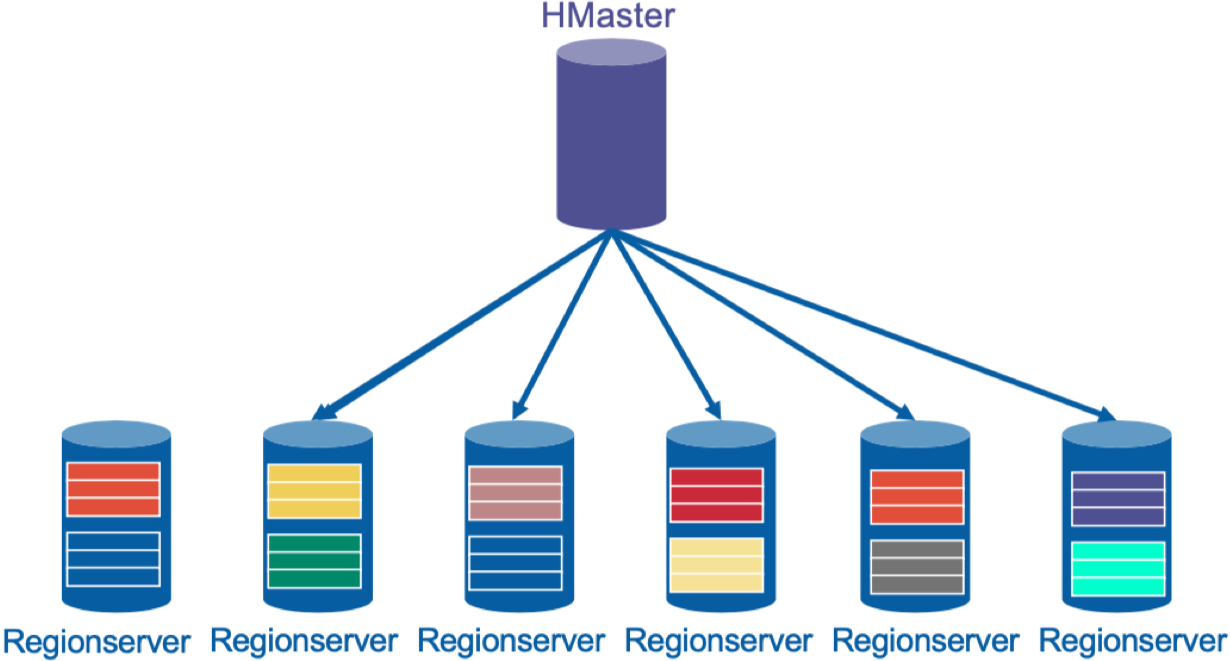
\includegraphics[width=0.7\textwidth]{Figures/HBaseNetworkTopology.jpeg}
    \caption{Network Topology of HBase.}\label{fig:HBNetTop}
\end{figure}

The HMaster and the RegionServers should be understood as pro- cesses running on the nodes, rather than the nodes themselves, even though it is common to use “HMaster” to designate the node on which the HMaster process runs, and “RegionServer” to designate a node on which a RegionServer process runs.

Remember, the namenode in HDFS does all the metalabel things. Creating directories, writing directories, deleting directories, etc. These are called DDL Operationd (Data Definition Language). The HMaster has other tasks than just that. It assigns regions to RegionServers. This means, for a given region (remember: interval of row IDs), all column families – each one within this region being a store – are handled by the same RegionServer.

There is no need to attribute the responsibility of a region to more than one RegionServer at a time because, as we will see soon, fault tolerance is already handled on the storage level by HDFS.

If a region grows too big, for example because of many writes in the same row ID interval, then the region will be automatically split by the responsible RegionServer. Note, however, that concentrated writes (“hot spots”) might be due to a poor choice of row IDs for the use case at hand. There are solution to this such as salting or using hashes in row ID prefixes.

If a RegionServer has too many regions compared to other Region-Servers, then the HMaster can reassign regions to other RegionServers.

Likewise, if a RegionServer fails, then the HMaster can reassign all its regions to other RegionServers.


\subsubsection{Physical Storage}
As we saw, the data is partitioned in stores, so we need to look at how each store is physically stored and persisted. The store is, physically, nothing less than an organized set of cells.

Each value in a cell is identified by a row ID (within the region handled by the store), a column family (the one handled by the store), a column qualifier (arbitrary) and a version (arbitrary). The version is often implicit as several versions of the same cell can co-exist with the latest one being current, but it is an important component in the identification of a value in a cell. This tuple of four values will be referred to as the key (of the value in the cell).

Each value in a cell is thus handled physically as a key-value pair where the key is a (row ID, column family, column qualifier, version) tuple.

All the cells within a store are eventually persisted on HDFS, in files that we will call HFiles. An HFile is, in fact, nothing else than a (boring) flat list of KeyVal- ues, one per version of a cell. What is important is that, in an HFile, all these KeyValues are sorted by key in increasing order, meaning, first sorted by row ID, then by column family (trivially unique for a given store), then by column qualifier, then by version (in decreasing order, recent to old). This means that all versions of a given cell that are in the same HFile are located together, and one of the values (within this HFile) is the latest.

HBase guarantees ACID on the row level (concurrent writes and reads are synchronizing with per-row locks). Clients therefore can access different rows at the same time, but two clients cannot access the same row simultaneously.

Of course, on the disk, a file is a sequence of 0s and 1s with no tabular structure, so that what in fact happens is that the KeyValues are stored sequentially. Now if we zoom in at the bit level, a KeyValue consists of four parts:
\begin{itemize}
    \item The length of the keys in bits (this length is encoded on a constant, known number of bits)
    \item The length of the value in bits (this length is encoded on a constant, known numbebr of bits)
    \item The actual key (of variable length)
    \item The actual value (of variable length)
\end{itemize}
The reason why we have the keylength and the valuelength at the beginning, is that the key and the value may hava variable lengths. Both, keylength and valuelength, are stored as 32 bits, thus 64 bits in total.

Zooming in even further, the key is itself made of the row ID, the column family, the column qualifier and the timestamp. We need also a row ID length and a column family length (similar to the key length and the value length). The timestamp has a fixed length (64 bits) and does not need additional input on its length. Finally the last byte (named “key type” for some reason) is mostly used as a deletion flag that indicates that the content of the cell, as of this version, was deleted. The reason why we don't need to specify the column qualifier length, is that we already know the key length, the row length and the column family length. Furthermore, the timestamp and the key type length are fixed. Thus, by simple subtraction, we obtain the column qualifier length.

\begin{figure}[h]
    \centering
    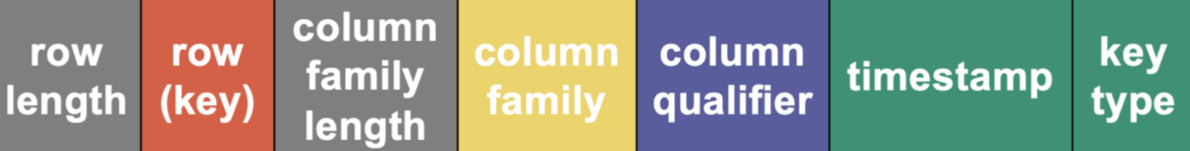
\includegraphics[width=0.7\textwidth]{Figures/KeyValueStructure.jpeg}
    \caption{Structure of a KeyValue}\label{fig:keyValStru}
\end{figure}

KeyValues, within an HFile, are organized in blocks. But to not confuse them with HDFS blocks, we will call them HBlocks. HBlocks have a size of 64 kB, but this size is variable: if the last KeyValue goes beyond this boundary, then the HBlock is simply longer and stops whenever the last KeyValue stops. The HFile then additionally contains an index of all blocks with their key boundaries. This separate index is loaded in memory prior to reading anything from the HFile. It can then be kept in memory for subsequent reads. Thanks to the index, it is possible to efficiently find out in which HBlock the KeyValues with a specific key (or within a specific key range) are to be read.

\begin{figure}[h]
    \centering
    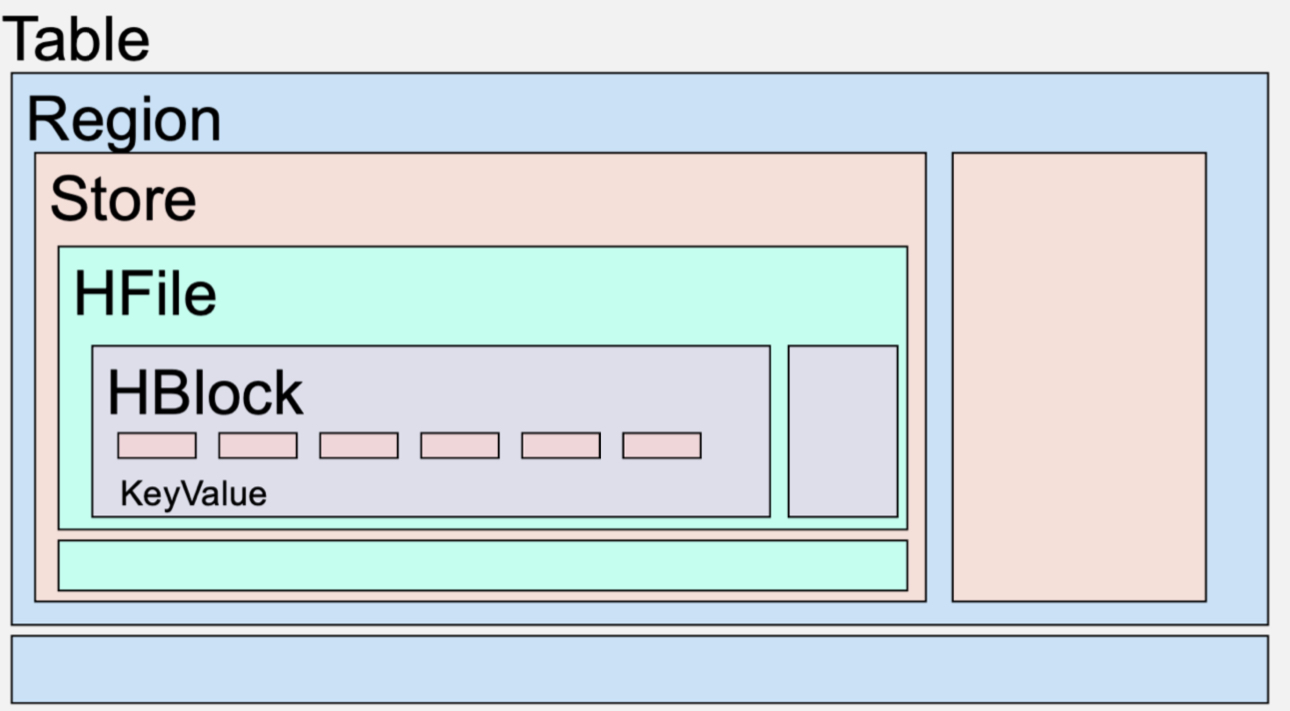
\includegraphics[width=0.7\textwidth]{Figures/SummaryPhysicalStorage.jpeg}
    \caption{Summary of the entire physical Storage hierarchy of KeyValues on HDFS.}\label{fig:SumPhysStor}
\end{figure}

There is one big problem. We can only write key-values in sorted order (append). How can we insert new values without having to rewrite the whole table?

\subsubsection{Log-structured merge trees}

Generally, “old” data is persisted to HDFS in HFiles, while “fresh” data is still in memory on the RegionServer node, and has not been persisted to HDFS yet. Thus, when accessing data, HBase needs to generally look every- where for cell values (i.e., physically, KeyValues) to potentially return: in every HFile, and in memory. As long as there is room in memory, freshly created KeyValues are added in memory. At some point, the memory becomes full (or some other limits are reached). When this happens, all the KeyValues need to be flushed to a brand new HFile. Upon flushing, all KeyValues are written sequentially to a new HFile in ascending key order, HBlock by HBlock, concurrently building the index structure. In fact, sorting is not done in the last minute when flushing. Rather, what happens is that when KeyValues are added to memory, they are added inside a data structure that maintains them in sorted order (such as tree maps) and then flushing is a linear traversal of the tree.

What happens if the machine crashes and we lose everything in memory? We have a so-called write-ahead-log for this. Before any fresh KeyValues are written to memory, they are written in sequential order (append) to an HDFS file called the HLog. There is one HLog per RegionServer. A full write-ahead-log also triggers a flush of all KeyValues in memory to a new HFile. If there is a problem and the memory is lost, the HLog can be retrieved from HDFS and “played back” in order to repopulate the memory and recreate the sorting tree structure.

Summary when to flush: Reaching max Memstore size in a store, reaching overall max Memstore size or reaching full write-ahead log.

After many flushes, the number of HFiles to read from grows and becomes impracticable. For this reason, there is an additional process called \textit{compaction} that takes several HFiles and outputs a single, merged HFile. Since the KeyValues within each HFile are already sorted, this can be done in linear time, as this is essentially the merge part of the merge-sort algorithm.

With flushing and compaction, we are starting to see some cycle of persistence. On a first level, the KeyValues in memory, on a second level, the KeyValues that have been flushed, on the third level, the KeyValues that have been flushed and compacted once, etc.

Compaction is not done arbitrarily but follows a regular, logarithmic pattern. Let us go through it. In a fresh HBase store, the memory becomes full at some point and a first HFile is output in a flush. Then the memory, which was emptied, becomes full again and a second HFile is output in a flush. This results in two HFiles of “standard size” that are immediately compacted to one HFile, twice as large. Then the memory, which was emptied, becomes full again and a new “standard-size” HFile is output in a flush. Then the memory, which was emptied, becomes full again and a second “standard-size” HFile is output in a flush. This results in two HFiles of “standard size” that are immediately compacted to one HFile, twice as large. This results in two HFiles of “double size” that are immediately compacted to one HFile, four times as large as the standard size. Then the memory, which was emptied, becomes full again and a new “standard-size” HFile is output in a flush. And so on...

\subsection{Additional design aspects}

\subsubsection{Bootstrapping lookups}
In order to know which RegionServer a client should communicate with to receive KeyValues corresponding to a specific region, there is a main, big lookup table that lists all regions of all tables together with the coor- dinates of the RegionServer in charge of this region as well as additional metadata (e.g. to support splitting regions, etc).
This big table is, in fact, also an HBase table, but it is special because this one fits on just one machine, known to everybody. Thus, the clients use this so-called meta table to know which RegionServers to communicate with.
To create, delete or update tables, clients communicate with the HMaster.

\subsubsection{Caching}
In order to improve latency, KeyValues that are normally persisted to HFiles (and thus no longer in memory) can be cached in a separate memory region, with the idea of keeping in the cache those KeyValues that are frequently accessed.
Caching is useless if we use batch processing, since in this case, we aggregate over the whole table anyway, or if we access the data randomly and uncontrolably.

\subsubsection{Bloom Filters}
HBase has a mechanism to avoid looking for KeyValues in every HFile. This mechanism is called a Bloom filter. It is basically a black box that can tell with absolute certainty that a certain key does not belong to an HFile, while it only predicts with good probability (albeit not certain) that it does belong to it. By maintaining Bloom filters for each HFile (or even each column), HBase can know with certainty that some HFiles need not be read when looking up certain keys.

\subsubsection{Data Locality and Short-Circuiting}
It is informative to think about the interaction between HBase and HDFS. In particular, recollect when we said that HDFS outputs the first replica of every block on the same (DataNode) machine as the client. Who is the client here? The RegionServer, which does co-habit with a DataNode. Now the pieces of the puzzle should start assembling in your mind: this means that when a RegionServer flushes KeyValues to a new HFile, a replica of each (HDFS) block of the HFile is written, by the DataNode process living on the same machine as the Region- Server process, to the local disk. This makes accessing the KeyValues in future reads by the RegionServer extremely efficient, because the RegionServer can read the data locally without communicating with the NameNode: this is known as short-circuiting in HDFS.

However, as time flies and the HDFS cluster lives its own life, some replicas might be moved to other DataNodes when rebalancing, making short-circuiting not (always) possible.
This, however, is not a problem, because with the log-structured merge tree mechanism, compactions happen regularly. And with every compaction, the replicas of the brand new HFile are again written on the local disk.



\pagebreak

\section{Data Models and Validation}

A data model is an abstract view over the data that hides the way it is stored physically. When going from the physical view (Syntax) to the logical view (Data Model) we speak about parsing and vice versa about serializing.

\subsection{The JSON Information Set}

The appropriate abstraction for any JSON document is a tree. The nodes of that tree, which are JSON logical values, are naturally of six possible kinds: the six syntactic building blocks of JSON. These are the four leaves corresponding to atomic values: Strings, Numbers, Booleans and Nulls. As well as two intermediate nodes (possibly leaves if empty): Objects (String-to-value map) and Arrays (List of values).

Formally, and not only for JSON but for all tree-based models, these nodes are generally called \textit{information items} and form the logical building blocks of the model, called \textit{information set}.

When a JSON document is being parsed by a JSON library, this tree is built in memory, the edges being pointers, and further processing will be done on the tree and not on the original syntax.

\subsection{The XML Information Set}

It is possible to do the same logical abstraction, also based on trees, with XML, where information items correspond to elements, attributes, text, etc.

A fundamental difference between JSON trees and XML trees is that for JSON, the labels (object keys) are on the edges connecting an object information item to each one of its children information items. In XML, the labels (these would be element and attribute names) are on the nodes (information items) directly. Another way to say it is that a JSON information item does not know with which key it is associated in an object (if at all), while an XML element or attribute information item knows its name.

\begin{figure}[h]
    \centering
    \begin{subfigure}{0.495\textwidth}
        \centering
        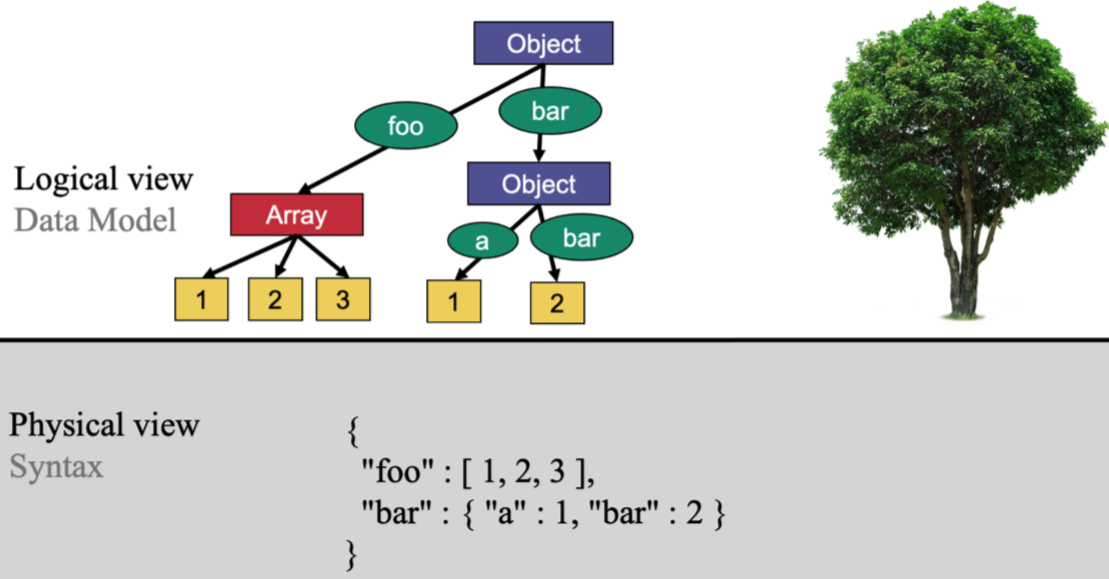
\includegraphics[width=\textwidth]{Figures/JSONTree.jpeg}
        \caption{JSON Tree}\label{subfig:JSONTree}
    \end{subfigure}
    \hfill
    \begin{subfigure}{0.495\textwidth}
        \centering
        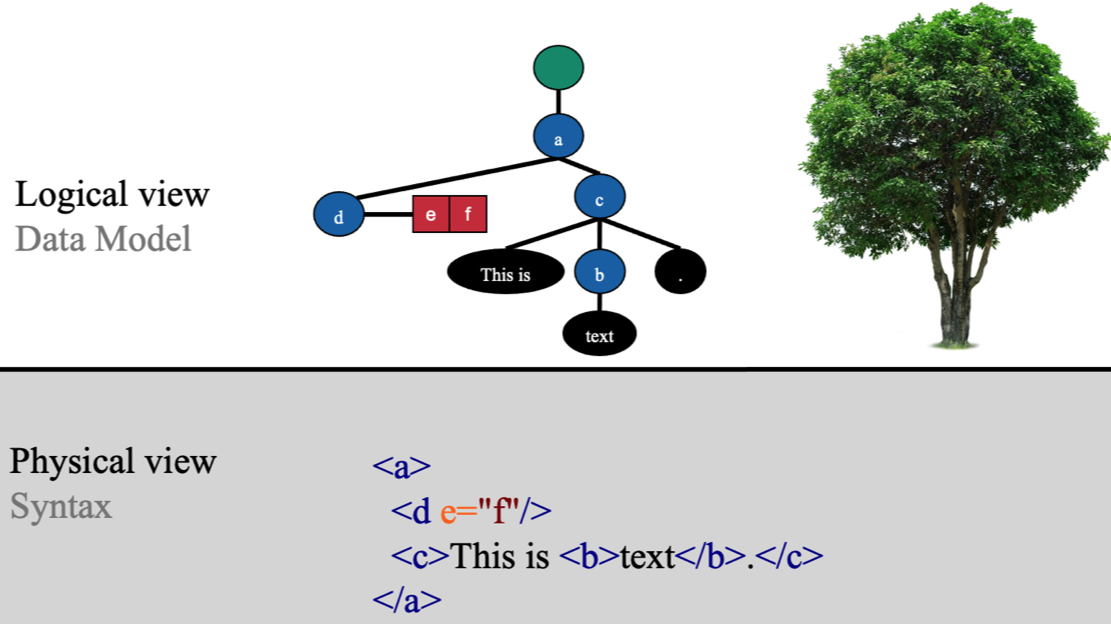
\includegraphics[width=\textwidth]{Figures/XMLTree.jpeg}
        \caption{XML Tree}\label{subfig:XMLTree}
    \end{subfigure}
    \caption{Tree Structures}\label{fig:Trees}
\end{figure}

There are many information items in XML. Here, we will focus on documents, elements, attributes and characters and discuss these based on the following example:

\begin{figure}[h]
    \centering
    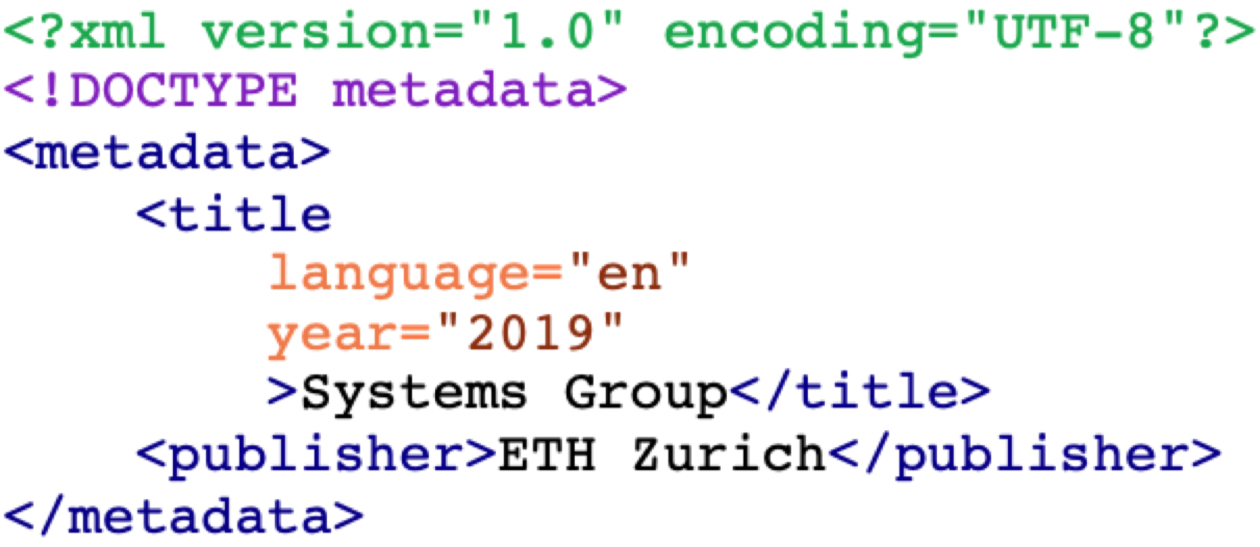
\includegraphics[width=0.6\textwidth]{Figures/XMLexplCode.jpeg}
    \caption{Example XML Document}\label{fig:XMLexpl}
\end{figure}

\subsubsection{Document Information Item}
The document information item is just the root of an XML tree. It does not correspond to anything syntactically or, if at all, it would correspond to the text and doctype declarations. In the example in \cref{fig:XMLexpl}, the documentation information has two important properties:
\begin{itemize}
    \item $\eckigeklammer{\text{children}}$ Element information item \textit{metadata}
    \item $\eckigeklammer{\text{version}}$ 1.0
\end{itemize}

\subsubsection{Element Information Item}
There is one element information item for each element. Here we have three.
The element information item \textit{metadata} has four important properties:
\begin{itemize}
    \item $\eckigeklammer{\text{local name}}$ metadata
    \item $\eckigeklammer{\text{children}}$ Element Information Item \textit{title}, Element Information Item \textit{publisher}
    \item $\eckigeklammer{\text{attribute}}$ (empty)
    \item $\eckigeklammer{\text{parent}}$ Document Information Item
\end{itemize}
The element information item \textit{title} has four important properties:
\begin{itemize}
    \item $\eckigeklammer{\text{local name}}$ title
    \item $\eckigeklammer{\text{children}}$ Character Information Item \textit{Systems Group}
    \item $\eckigeklammer{\text{attributes}}$ Attribute Information Item \textit{language}, Attribute Information Item \textit{year}
    \item $\eckigeklammer{\text{parent}}$ Element Information Item \textit{metadata}
\end{itemize}
The element information item \textit{publisher} has four important properties:
\begin{itemize}
    \item $\eckigeklammer{\text{local name}}$ publisher
    \item $\eckigeklammer{\text{children}}$ Character Information Item \textit{ETH Zurich}
    \item $\eckigeklammer{\text{attribute}}$ (empty)
    \item $\eckigeklammer{\text{parent}}$ Element Information Item \textit{metadata}
\end{itemize}

\subsubsection{Attribute Information Item}
There is one attribute information item for each attribute. Here we have two.
The attribute information item \textit{language} has three important properties:
\begin{itemize}
    \item $\eckigeklammer{\text{local name}}$ language
    \item $\eckigeklammer{\text{normalized value}}$ en
    \item $\eckigeklammer{\text{owner element}}$ Element Information Item \textit{title}
\end{itemize}
The attribute information item \textit{year} has three important properties:
\begin{itemize}
    \item $\eckigeklammer{\text{local name}}$ year
    \item $\eckigeklammer{\text{normalized value}}$ 2019
    \item $\eckigeklammer{\text{owner element}}$ Element Information Item \textit{title}
\end{itemize}

\subsubsection{Character and Text Information Item}
There are as many character information items as characters in text (between tags). For example, for the S in Systems Group:
\begin{itemize}
    \item $\eckigeklammer{\text{character code}}$ the unicode code point for the letter S
    \item $\eckigeklammer{\text{parent}}$ Element Information Item \textit{title}
\end{itemize}
It is sometimes simpler to group them into a single (non standard) text information item:
\begin{itemize}
    \item $\eckigeklammer{\text{characters}}$ S y s t e m s $<$space$>$ G r o u p
    \item $\eckigeklammer{\text{parent}}$ Element Information Item \textit{title}
\end{itemize}

\subsubsection{The entire tree}
All information items built previously can finally be assembled and drawn as a tree. The edges, corresponding to children and parent (or owner element) properties, will correspond to pointers in memory when the tree is built by the XML library:

\begin{figure}[h]
    \centering
    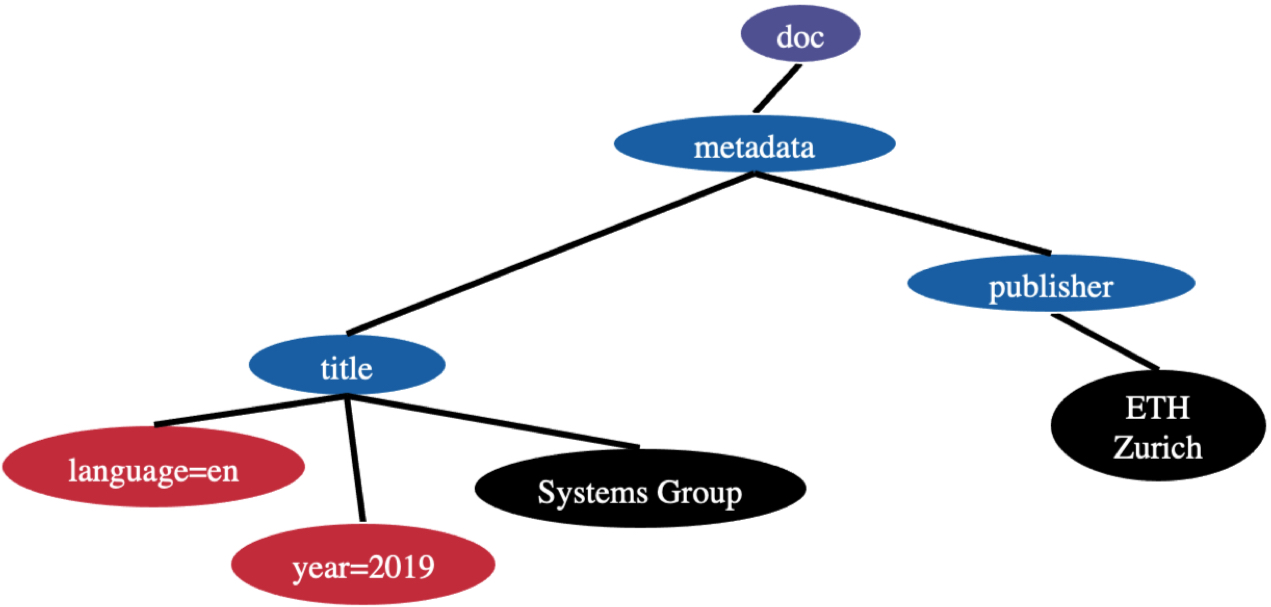
\includegraphics[width=0.5\textwidth]{Figures/XMLTree2.jpeg}
    \caption{Assembled XML Tree.}\label{fig:XMLTree2}
\end{figure}

\subsection{Validation}
Validation is not the same as well-formedness.
Once documents, JSON or XML, have been parsed and logically abstracted as a tree in memory, the natural next step is to check for further structural constraints.

For example, you could want to check whether your JSON documents all associate key “name” with a string, or if they all associate “years” with an array of positive integers. Or you could want to check whether your XML documents all have root elements called “persons,” and whether the root element in each document has only children elements called “person,” all with an attribute “first” and an attribute “last.”

This might remind the reader of schemas in a relational database, but with a major difference: in a relational database, the schema of a table is defined before any data is populated into the table. Thus, the data in the table is guaranteed, at all times, to fulfil all the constraints of the schema. The exact term is that the data is guaranteed to be valid against the schema, because the schema was enforced at write time (schema on write).

But in the case of a collection of JSON and XML documents, this is the other way round. A collection of JSON and XML documents out there can exist without any schema and contain arbitrary structures. Validation happens “ex post,” that is, only after reading the data (schema on read).

Thus, it means that JSON and XML documents undergo two steps:
\begin{itemize}
    \item a well-formedness check: attempt to parse the document and consruct a tree representation in memory
    \item (if the first step succeeded) a validation check given a specific schema
\end{itemize}
Validation is schema dependent: a given well-formed document can be valid against schema A and invalid against schema B.

Validation is often performed on much more than a document at a time: an entire collection. Thus, we distinguish between heterogeneous collections, whose documents are not valid against any particular schema, and homogeneous collections, whose documents are all valid against a specific schema.

\subsection{Item Types}
A fundamental aspect of validation is the type system. A well-designed type system, in turn, allows for storing the data in much more efficient, binary formats tailored to the model.

The first aspect that almost all, if not all type systems, have in common, is the distinction between atomic types and structured types.

\subsubsection{Atomic Types}
Atomic types correspond to the leaf of a tree data model: these are types that do not contain any further nestedness.

\subsubsection*{Strings}
Strings are simply finite sequences of (usually printable) characters. Formally, strings form a monoid under concatenation, where the neutral element is the empty string.

All atomic types have in common that they have a logical value space and a lexical value space. The logical value space corresponds to the actual logical abstraction of the type (e.g., a mathematical set of integers), while the lexical value space corresponds to the representation of logical values in a textual format (such as the decimal, or binary, or hexadecimal representation of an integer).

Often, the lexical representation of a string is double-quoted, sometimes also single-quoted.

The difference between the lexical representation and the logical value of a string becomes immediately apparent when escaping is used. For example, the lexical representation "$\backslash \backslash \backslash$" corresponds to the (logical) string "$\backslash$".

\subsubsection*{Numbers}

\paragraph{Integers}
In older programming languages, support for integers used to be bounded. This is why classical types, still in use today, correspond to 8-bit (often called byte), 16-bit (often called short), 32-bit (often called int) and 64-bit integers (often called long). This means that, expressed in base 2, they use 8, 16, 32 or 64 bits (binary digits).
However, in modern databases, it is customary to support unbounded integers.

The lexical representation of integers is usually done is base 10, in the familiar decimal system, even though base 2, 8 or 16 can be found, too. Leading 0s are optional, but when an logical integer value is canonically serialized, it is done without a leading 0.

\paragraph{Decimals}
Decimals correspond to real numbers that can be written as a finite sequence of digits in base 10, with an optional decimal period. Equivalently, these are fractions that can be expressed with a power of 10 in the denominator.
Many modern databases or storage formats support the entire logical decimal value space with no restriction on how large, small or precise a decimal number is.

The number of digits in the whole decimal number is called the precision and the number of digits behind the comma is called the scale.

\paragraph{Floating-Point}
Floating-point numbers are limited both in precision and magnitude (both upper and lower) in order to fit on 32 bits (float) or 64 bits (double). Floats have about 7 digits of precision and their absolute value can be between roughly $10^{-37}$ and $10^{37}$, while doubles have 15 digits of precision and their absolute value can be between roughly $10^{-307}$ and $10^{308}$.

Double and float types also cover additional special values: NaN (not a number), positive and negative infinity, and negative zero (in addition to the “positive” 0).

The lexical representation of floats and doubles often use the scientific notation: \texttt{-12.34E-56}.
And the lexical values corresponding to the special logical values look like so: \texttt{NaN}, \texttt{INF}, \texttt{-INF}, \texttt{-0}.


\paragraph{Booleans}
The logical value space for the Boolean type is made of two values: true and false as in NoSQL queries, two-valued logic is typically assumed.
The corresponding lexical values are typically \texttt{true} and \texttt{false}.

\paragraph{Dates and Times}
Dates are commonly using the Gregorian calendar with a year (BC or AD), a month and a day of the month. Dates require quotes!

Times are expressed in the hexagesimal (60) basis with hours, minutes, seconds, where the seconds commonly go all the way to microseconds (six digits after the decimal period).

Datetimes are expressed with a year, a month, a day of the month, hours, minutes and (decimal) seconds.

The timestamp type corresponds to a datetime with a timezone, but treating datetimes as equivalent if they express the same point in time. Timestamp values are typically stored as longs (64-bit integers) expressing the number of milliseconds elapsed since January 1, 1970 by convention.

The lexical values can also vary, although many technologies follow the ISO 8601 standard, where lexical values look like so (with many parts optional): \texttt{2022-08-07T14:18:00.123456+02:00}, \texttt{2022-08-07}, \texttt{14:18:00.123456}, \texttt{14:18:00.123456Z}.

\paragraph{Durations}
Durations can be of many different kinds, generally a combination of years, months, days, hours, minutes and (possibly with decimals) seconds.
What is important to understand is that there is a “wall” between months and days: what is the duration “1 month and 1 day?” It could be 29, 30, 31, or 32 days and should thus be avoided. Thus, most durations, for the sake of being unambiguous, are either involving years and/or months, or are involving days and/or hours and/or minutes and/or seconds.

The lexical representation can vary, but there is a standard defined by ISO 8601 as well, starting with a P and prefixing sub-day parts with a T. Here some examples:
\begin{itemize}
    \item 2 years and 3 months: \texttt{P2Y3M}
    \item 4 days, 3 hours, 2 minutes and 1.123456 seconds: \texttt{P4DT3H2M1.123456}
    \item 3 hours, 2 minutes and 1.123456 seconds: \texttt{PT3H2M1.123456}
\end{itemize}

\paragraph{Binary Data}
Binary data is, logically, simply a sequence of bytes. There are two main lexical representations used in data: hexadecimal and base64. Hexadecimal expresses the data with two hexadecimal digits per byte, like so: \texttt{0123456789ABCDEF} which would correspond to the bit sequence:

\texttt{0000000100100011010001010110011110001001101010111100110111101111}.

\paragraph{Null}
Many technologies and formats also provide support for null values, although how this is done largely varies. Some technologies allow null to appear as a (valid) value for any type. A schema can either allow, or disallow the null value. Often, the terminology used is that a type can be nullable (or nillable) or not. Other technologies consider that there is a singleton-valued null type, containing only the null value with the lexical representation \texttt{null}.

Allowing nulls is done by taking the union of the desired type with the null type. Yet other technologies consider null when it appears as a value in an object to be semantically equivalent by the absence of a value and then, allowing or disallowing null is achieved by (e.g. in JSON) making the field required or optional. It is important to understand that the latter technologies are unable to distinguish between the following two JSON objects, so that information in the input dataset is lost upon validating:

\begin{lstlisting}[style=json, label={lst:jsonnull}]
{}
{ "foo" : null }
\end{lstlisting}

This can be problematic with datasets where this distinction is semantically relevant. XML also supports null values, but calls them “nil” and does so with a special attribute and no content rather than with a lexical representation

\begin{lstlisting}[style=xml, label={lst:xmlnull}]
<foo
    xmlns:xsi="http://www.w3.org/2001/XMLSchema-instance"
    xsi:nil="true"/>
\end{lstlisting}

\subsubsection{Structured Types}
The two main types are:
\begin{itemize}
    \item Lists. E.g. JSON Array, XML Element, DataFrame Array.
    \item Maps. E.g. JSON Object, Set of XML Attributes, DataFrame Struct.
\end{itemize}

\paragraph{Type Names}
Below there is a summary of many types over various technologies and languages and how they correspond to each other. The most important thing to see here is that on the high level, atomic types are almost always the same everywhere, even though the names can vary.

\begin{figure}[h]
    \centering
    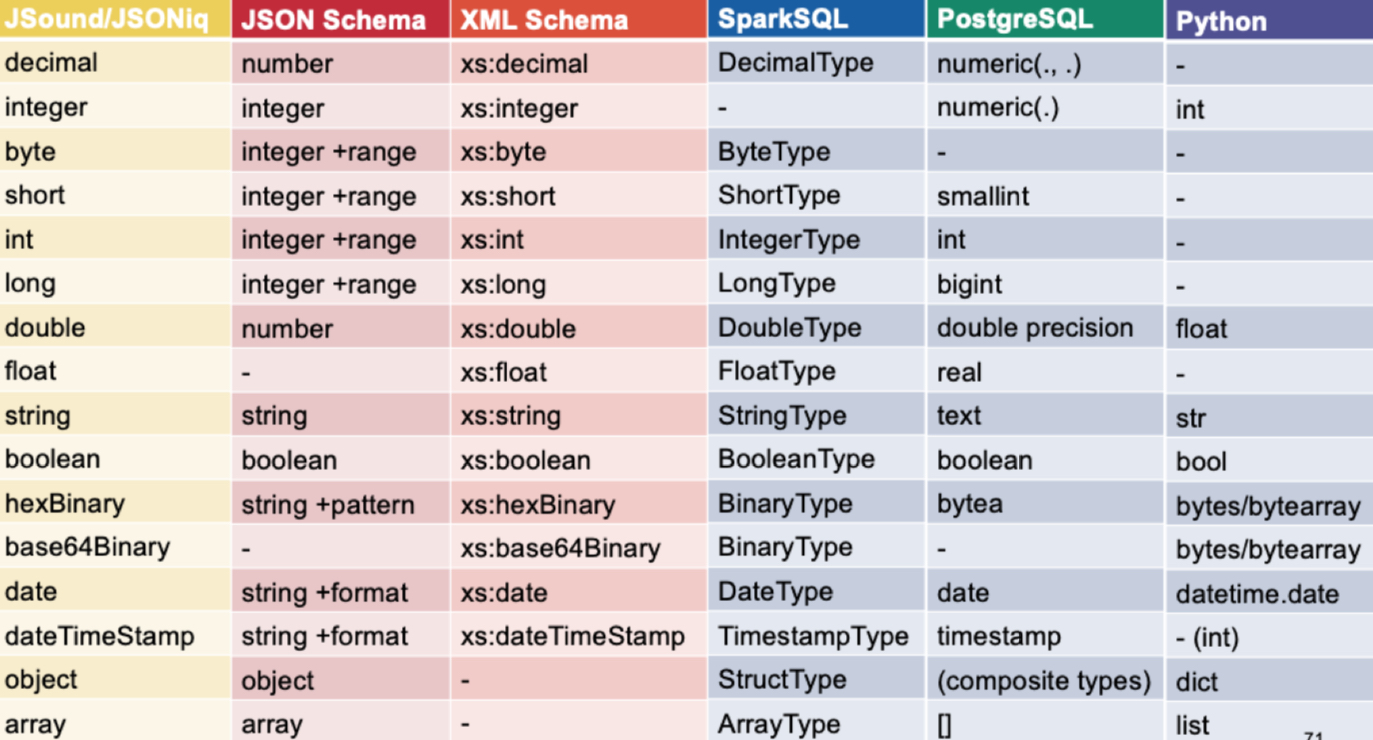
\includegraphics[width=0.9\textwidth]{Figures/TypeNames.jpeg}
    \caption{Type Names}\label{fig:TypeNames}
\end{figure}


\subsection{Sequence Types}

\paragraph{Cardinality}
In the context of data querying but also of nested lists and arrays, items (single values) rarely appear alone. They often appear as a sequence of many values. Thus, many type system give options regarding the number of occurrences of items in a sequence. There are four main occurrence indicators:
\begin{itemize}
    \item ust once (often implicit): exactly one item. Common adjective: required
    \item optional: zero or one item. Often represented witha question mark (?). Common adjective: optional
    \item any occurence: zero, one or more items. Often represented with a Kleen star (*). Common adjective: repeated
    \item at least once: one or more items. Often represented with a Kleene plus (+).
\end{itemize}

\subsection{JSON Validation / JSOUND}

\subsubsection{Validating flat objects}
A JSound-schema pair may look like this:

\begin{minipage}{0.45\textwidth}
\begin{lstlisting}[style=json,caption={JSON Code}]
{
    "name" : "Einstein",
    "first" : "Albert",
    "age" : 142
}
\end{lstlisting}
\end{minipage}
\hfill
\begin{minipage}{0.45\textwidth}
\begin{lstlisting}[style=json,caption={JSOUND Schema}]
{
    "name" : "string",
    "first" : "string",
    "age" : "integer"
}
\end{lstlisting}
\end{minipage}
“string” can be replaced with any other named type, in particular taken from the table shown in the former section. Let us list them here:
\begin{itemize}
    \item Strings: string, anyURI (for strings containing a URI);
    \item Numbers: decimal, integer, float, double, long, int, short, byte, negativeInteger, positiveInteger, nonNegativeInteger, nonPositiveInteger, unsignedByte, unsighedShort, unsignedInt, unsignedLong;
    \item Dates and times: date, time, dateTime, gYearMonth, gYear, gMonth, gDay, gMonthDay, dateTimeStamp;
    \item Time intervals: duration, yearMonthDuration, dayTimeDuration;
    \item Binary types: hexBinary, base64Binary
    \item Booleans: boolean
    \item Nulls: null
\end{itemize}
Alternatively to JSound, one can use JSON Schema for validation. The JSON Schema for the above JSON code is
\begin{lstlisting}[style=json,caption={Schema}]
{
    "type" : "object",
    "properties" : {
        "name" : "string",
        "first" : "string",
        "age" : "number"
    }
}
\end{lstlisting}
The available JSON Schema types are string, number, integer, boolean, null, array and object. This closely matches the original JSON syntax with the only exception that numbers have this additional integer subtype. The type system of JSON Schema is thus less rich than that of JSound, but extra checks can be done with so-called formats, which include date, time, duration, email, and so on including generic regular expressions. Like JSound, JSON Schema also allow restricting the length of a string, constraining numbers to intervals, etc.

\subsubsection{Requiring the presence of a key}
By default, the presence of a key is optional, so that each one of the following objects is also valid against the previous schema:
\begin{lstlisting}[style=json]
{ "name" : "Einstein" }
{ "first" : "Albert" }
{ "age" : 142 }
{ "name" : "Einstein", "age" : 142 }
{}
\end{lstlisting}
It is possible to require the presence of a key by adding an exclamation mark, like so.
\begin{lstlisting}[style=json]
{
"!name" : "string",
"!first" : "string",
"age" : "integer"
}
\end{lstlisting}
This is the equivalent JSON Schema, which uses a “required” property associated with the list of required keys to express the same:
\begin{lstlisting}[style=json]
{
    "type" : "object",
    "required" : [ "name", "first" ]
    "properties" : {
        "name" : "string",
        "first" : "string",
        "age" : "number"
    }
}
\end{lstlisting}

\subsubsection{Open and closed object types}
In the JSound compact syntax, extra keys are forbidden. The schema is said to be closed. There are ways to define JSound schemas to allow arbitrary additional keys (open schemas), with a more verbose syntax. Unlike JSound, in JSON Schema, extra properties are allowed by default. JSON Schema then allows to forbid extra properties with the “additionalProperties” property, like so:
\begin{lstlisting}[style=json]
{
    "type" : "object",
    "required" : [ "name", "first" ]
    "properties" : {
        "name" : "string",
        "first" : "string",
        "age" : "number"
    },
    "additionalProperties" : false
}
\end{lstlisting}

\subsubsection{Nested Structures}
Examples of nested schemas:
\begin{lstlisting}[style=json]
{ "numbers" : [ "integer" ] }
\end{lstlisting}
\begin{lstlisting}[style=json]
{ "matrix" : [ [ "decimal" ] ] }
\end{lstlisting}
Examples of valid JSON code for these two schemas:
\begin{lstlisting}[style=json]
{
    "numbers" : [ 1, 2, 6, 2, 7, 1, 57, 4 ]
}
\end{lstlisting}
\begin{lstlisting}[style=json]
{ "matrix" : [ [ 0, 1 ], [ 1, 0 ] ] }
\end{lstlisting}

With the JSound compact syntax, object and array types can nest arbitrarily:
\begin{lstlisting}[style=json]
{
    "datapoints" : [
        {
            "features" : [ "double" ],
            "label" : "integer"
        }
    ]
}
\end{lstlisting}

\vspace{1\baselineskip}

Every schema can be given a name, turning into a type. When a document is valid against a schema, it is typical to also annotate the document, which means that its tree representation in memory contains additional type information and values are stored natively in their type, enabling efficient processing and space efficiency.

JSound allows for the definition not only of arbitrary array and object types as shown above, but also of additional atomic types, by imposing some constraint on existing types (e.g., airport codes by restricting the length of a string to 3 and requiring all three characters to be uppercase letters, shoe sizes with intervals, etc). These are called user-defined types.

\subsubsection{Primary key constraints, allowing for null, default values}
There are a few more features available in the compact JSound syntax (not in JSON Schema) with the special characters @, ? and =:

\begin{lstlisting}[style=json]
{
    "datapoints" : [
        {
            "@id" : "int",
            "features" : [ "double" ],
            "label?" : "integer",
            "set" : "string=training"
        } 
    ]
}
\end{lstlisting}
The question mark (?) allows for null values (which are not the same as absent values). Technically, it creates a union of the specified type with the null type.
The arobase (@) indicates that one or more fields are primary keys for a list of objects that are members of the same array. In this case, it means all id fields must be different for the datapoints array of each document.
The equal sign (=) is used to indicate a default value that is automatically populated if the value is absent. In this case, if the field “set” is missing, then upon annotating the document after its validation, it will be added with a value “training”.

\subsubsection{Accepting any values}
Accepting any values in JSound can be done with the type “item”, which contains all possible values, like so:
\begin{lstlisting}[style=json]
{
    "!name" : "item",
    "!first" : "item",
    "age" : "number"
}
\end{lstlisting}
In JSON Schema, in order to declare a field to accept any values, you can use either true or an empty object in lieu of the type, like so:
\begin{lstlisting}[style=json]
{
  "type" : "object",
  "required" : [ "name", "first" ]
  "properties" : {
        "name" : {},
        "first" : true,
        "age" : "number"
    },
  "additionalProperties" : false
}
\end{lstlisting}
JSON Schema additionally allows to use false to forbid a field.

\subsubsection{Type Unions}
In JSON Schema, it is also possible to combine validation checks with Boolean combinations.
First, disjunction (logical or) is done with
\begin{lstlisting}[style=json]
{
    "anyOf" : [
        { "type" : "string" },
        { "type" : "array" }
    ]
}
\end{lstlisting}
JSound schema allows defining unions of types with the vertical bar inside type strings, like so: \texttt{"string|array"}.

\subsubsection{Type conjunction, exclusive or, negation}
In JSON Schema only (not in JSound), it is also possible to do a conjunction (logical and) with
\begin{lstlisting}[style=json]
{
    "allOf" : [
        { "type" : "string", "maxLength" : 3 },
        { "type" : "string", "minLength" : 2 }
    ]
}
\end{lstlisting}
as well as exclusive or (xor):
\begin{lstlisting}[style=json]
{
"oneOf" : [
    { "type" : "number", "minimum" : 2  },
    { "type" : "number", "multipleOf" : 2 }
  ]
}
\end{lstlisting}
as well es negation:
\begin{lstlisting}[style=json]
{
  "not" : { "type" : "array" }
}
\end{lstlisting}

\subsubsection{Summary}
In summary, you can either restrict values to a specific type, make an implicit cast, require a value or have open object types and closed object types.


\subsection{XML Validation}

XML validatino is also supported by several technologies. Here, we will look at XML Schema.

\subsubsection{Simple Types}

In \cref{lst:XMLSchemaCode,lst:XMLSchema} we can see a simple XML Code and XML Schema pair.

\begin{lstlisting}[style=XML,caption={XML Code},label={lst:XMLSchemaCode}]
<?xml version="1.0" encoding="UTF-8"?>
<foo>This is text.</foo>
\end{lstlisting}

\begin{lstlisting}[style=XML,caption={XML Schema},label={lst:XMLSchema}]
<?xml version="1.0" encoding="UTF-8"?>
<xs:schema xmlns:xs="http://www.w3.org/2001/XMLSchema">
    <xs:element name="foo" type="xs:string"/>
</xs:schema>
\end{lstlisting}

Notice that all elements in an XML Schema are in a namespace, the XML Schema namespace. The top element in an XML Schema document is the xs:schema element, and inside there is an element declaration done with the xs:element element. It has two attribute: one defines the name of the element to validate (foo) and the other one specifies its type (xs:string). The list of predefined atomic types is the same as in JSound, except that in XML Schema, all these predefined types live in the XML Schema namespace and thus bear the prefix xs as well.

\subsubsection{Simple Types}
The most important built-in types are: strings, numbers, dates and times, time intervals, binary types, booleans and nulls.

XML Schema allows you to define user-defined atomic types, for example restricting the length of a string to 3 for airport codes, and then use it with an element:

\begin{lstlisting}[style=XML,caption={XML Schema for Airport Codes}]
<?xml version="1.0" encoding="UTF-8"?>
<xs:schema xmlns:xs="http://www.w3.org/2001/XMLSchema">
    <xs:simpleType name="airportCode">
        <xs:restriction base="xs:string">
            <xs:length value="3"/>
        </xs:restriction>
    </xs:simpleType>
    <xs:element name="foo" type="airportCode"/>
</xs:schema>
\end{lstlisting}

\begin{lstlisting}[style=XML,caption={Valid XML Code with the above Schema for Airport Codes}]
<?xml version="1.0" encoding="UTF-8"?>
<foo>
    ZRH
</foo>
\end{lstlisting}

\subsubsection{Complex Types}
It is also possible to constrain structures and the element/attribute/text hierarchy with complex types applying to element nodes. There are four main kinds of complex types:
\begin{itemize}
    \item complex content: there can be nested elements, but there can be no text nodes as direct children.
    \item simple content: there are no nested elements: just text, but attributes are also possible.
    \item empty content: there are neither nested elements nor text, but attributes are also possible.
    \item mixed content: there can be nested elements and it can be intermixed with text as well.
\end{itemize}

\begin{lstlisting}[style=XML,caption={XML Code Example with complex content.}]
<foo>
    <twotofour>foobar</twotofour>
    <twotofour>foobar</twotofour>
    <twotofour>foobar</twotofour>
    <zeroorone>true</zeroorone>
</foo>
\end{lstlisting}

\begin{lstlisting}[style=XML,caption={XML Schema for the above Example with complex content.}]
<?xml version="1.0" encoding="UTF-8"?>
<xs:schema xmlns:xs="http://www.w3.org/2001/XMLSchema">
    <xs:complexType name="complex">
        <xs:sequence>
            <xs:element
                name="twotofour"
                type="xs:string"
                minOccurs="2"
                maxOccurs="4"/>
            <xs:element
                name="zeroorone"
                type="xs:boolean"
                minOccurs="0"
                maxOccurs="1"/>
        </xs:sequence>
    </xs:complexType>
    <xs:element name="foo" type="complex"/>
</xs:schema>
\end{lstlisting}

Note how children elements can be repeated, and the number of occurrences can be constrained to some interval with minOccurs and maxOccurs attributes in the schema. Of course, this all works recur- sively, i.e., the nested elements can also have complex types with com- plex content and so on (even though in this example they have simple types).

\begin{lstlisting}[style=XML,caption={XML Code Example with simple content.}]
<foo country="Switzerland">2014-12-02</foo>
\end{lstlisting}

\begin{lstlisting}[style=XML,caption={XML Schema for the above Example with simple content.}]
<?xml version="1.0" encoding="UTF-8"?>
<xs:schema xmlns:xs="http://www.w3.org/2001/XMLSchema">
    <xs:complexType name="dateCountry">
    <xs:simpleContent>
        <xs:extension base="xs:date">
            <xs:attribute name="country" type="xs:string"/>
        </xs:extension>
    </xs:simpleContent>
    </xs:complexType>
    <xs:element name="foo" type="dateCountry"/>
</xs:schema>
\end{lstlisting}

Note how a complex type with simple content is defined as the extension of a simple type, adding one or more attributes to it. If there are no attributes, of course, there is no need to bother with a complex type: a simple type does the trick as shown before.


\begin{lstlisting}[style=XML,caption={XML Code Example with empty content.}]
<foo/>
\end{lstlisting}

\begin{lstlisting}[style=XML,caption={XML Schema for the above Example with empty content.}]
<?xml version="1.0" encoding="UTF-8"?>
<xs:schema xmlns:xs="http://www.w3.org/2001/XMLSchema">
    <xs:complexType name="complex">
        <xs:sequence/>
    </xs:complexType>
    <xs:element name="foo" type="complex"/>
</xs:schema>
\end{lstlisting}


\begin{lstlisting}[style=XML,caption={XML Code Example with mixed content.}]
<foo>Some text and some <b>bold</b> text.</foo>
\end{lstlisting}

\begin{lstlisting}[style=XML,caption={XML Schema for the above Example with mixed content.}]
<?xml version="1.0" encoding="UTF-8"?>
<xs:schema xmlns:xs="http://www.w3.org/2001/XMLSchema">
    <xs:complexType name="mixedContent" mixed="true">
        <xs:sequence>
            <xs:element
                name="b"
                type="xs:string"
                minOccurs="0"
                maxOccurs="unbounded"/>
        </xs:sequence>
    </xs:complexType>
    <xs:element name="foo" type="mixedContent"/>
</xs:schema>
\end{lstlisting}

\subsubsection{Attribute declarations}
Attributes always have a simple type.

\begin{lstlisting}[style=XML,caption={XML Code Example with empty content with one attribute.}]
<foo country="Switzerland"/>
\end{lstlisting}

\begin{lstlisting}[style=XML,caption={XML Schema for the above Example with empty content with one attribute.}]
<?xml version="1.0" encoding="UTF-8"?>
<xs:schema xmlns:xs="http://www.w3.org/2001/XMLSchema">
    <xs:complexType name="withAttribute">
        <xs:sequence/>
        <xs:attribute name="country"
            type="xs:string"
            default="Switzerland"/>
    </xs:complexType>
    <xs:element name="foo" type="withAttribute"/>
</xs:schema>
\end{lstlisting}

The default attribute of the attribute declaration will automatically add an attribute with the corresponding name and specified value in memory in case it was missing in the original instance. This works just like in JSound.


\subsection{Data Frames}
There is a particular subclass of semi-structured datasets that are very interesting: valid datasets, which are collections of JSON objects valid against a common schema, with some requirements on the considered schemas.
The datasets belonging to this particular subclass are called data frames, or dataframes.

Specifically, for the dataset to qualify as a data frame, firstly, we forbid schemas that allow for open object types, that is, schemas must disallow any additional attributes, and, secondly, we forbid schemas that allow for object or array values to be too permissive and allow any values, that is, we ask that schemas require specific types such as integers, strings, dates, objects representing a person, arrays of binaries, etc. We, however, include schemas that allow for null values and/or absent values.

Under the above conditions, we call the collection of objects a data frame. It should be immediate to the reader that relational tables are data frames, while data frames are not necessarily relational tables: data frames can be (and are often) nested, but they are still relatively homogeneous to some extent. Relatively, because schemas can still allow for a value to be missing.

Data frames have the nice property that they can be drawn visually in structures that look like generalized relational tables and that look a bit nicer and more structured that the previous visuals with nested tables. Further, JSound compact schemas provides a natural syntax for constraining data frames, because object types in this syntax are always closed, and it allows for requiring or not values, and for including or not null values. Thus, we can now give a few examples of JSound schemas and their corresponding visuals.

Here are some examples of JSound schema with the corresponding visual representation.

\begin{minipage}{0.45\textwidth}
\vspace{1\baselineskip}
\begin{lstlisting}[style=json,caption={"flat" JSound Schema}]
{
    "ID" : "integer",
    "Name" : "string",
    "Living" : "boolean"
}      
\end{lstlisting}
\end{minipage}
\hfill
\begin{minipage}{0.45\textwidth}
\begin{table}[H]
    \centering
    \begin{tabular}{|l|l|l|}
        \hline ID & Name & Living \\
        \hline 1 & Einstein & false \\
        \hline 2 & Penrose & true \\
        \hline 3 & Turing & false \\
        \hline 4 & Dean & true \\
        \hline
    \end{tabular}
    \caption{Visualization of "flat" JSound Schema}
\end{table}
\end{minipage}

\begin{minipage}{0.45\textwidth}
\vspace{1\baselineskip}
\begin{lstlisting}[style=json,caption={Denormalized JSound Schema with an array of strings.}]
{
    "ID" : "integer",
    "Name" : [ "string" ],
    "Living" : "boolean"
}   
\end{lstlisting}
\end{minipage}
\hfill
\begin{minipage}{0.45\textwidth}
\begin{table}[H]
    \centering
    \begin{tabular}{|l|l|l|}
        \hline ID & Name & Living \\
        \hline 1 & Albert & false \\
        \cline { 2 - 2 } & Einstein & \\
        \hline 2 & Penrose & true \\
        \hline 3 & Alan & false \\
        \cline { 2 - 2 } & Turing & \\
        \hline 4 & Dean & true \\
        \hline
    \end{tabular}
    \caption{Visualization of denormalized JSound Schema with an array of strings.}
\end{table}
\end{minipage}


\begin{minipage}{0.45\textwidth}
\vspace{1\baselineskip}
\begin{lstlisting}[style=json,caption={Denormalized JSound Schema with nested objects.}]
{
    "ID" : "integer",
    "Name" : {
        "First" : "string",
        "Last" : "string"
    },
    "Living" : "boolean"
}
\end{lstlisting}
\end{minipage}
\hfill
\begin{minipage}{0.45\textwidth}
\begin{table}[H]
    \centering
    \begin{tabular}{|l|l|l|l|}
        \hline \multirow{2}{*}{ ID } & \multicolumn{2}{|l|}{ Name } & \multirow{2}{*}{ Living } \\
        \cline { 2 - 3 } & First & Last & \\
        \hline 1 & Albert & Einstein & false \\
        \hline 2 & Roger & Penrose & true \\
        \hline 3 & Alan & Turing & false \\
        \hline 4 & Jeff & Dean & true \\
        \hline
    \end{tabular}
    \caption{Visualization of denormalized JSound Schema with an nested objects.}
\end{table}
\end{minipage}


\begin{minipage}{0.45\textwidth}
\begin{lstlisting}[style=json,caption={Denormalized JSound Schema with objects nested in arrays.}]
{
    "ID" : "integer",
    "Who" : [
        {
            "Name" : "string",
            "Type" : "string"
        }
    ],
    "Living" : "boolean"
}
\end{lstlisting}
Alternative:
\begin{lstlisting}[style=json,caption={Denormalized JSound Schema with objects nested in arrays.}]
{
    "ID" : "integer",
    "Who" : {
        "Name" : [ "string" ],
        "Type" : [ "string" ]
    },
    "Living" : "boolean"
}
\end{lstlisting}
\end{minipage}
\hfill
\begin{minipage}{0.45\textwidth}
\begin{table}[H]
    \centering
    \begin{tabular}{|l|l|l|l|}
        \hline ID & \multicolumn{2}{|l|}{ Who } & Living \\
        \cline{ 2 - 3 } & Name & Type & \\
        \hline 1 & Albert & first & false \\
        \cline{ 2 - 3 } & Einstein & last & \\
        \hline 2 & Penrose & last & true \\
        \hline 3 & Alan & first & false \\
        \cline{ 2 - 3 } & Turing & last & \\
        \hline 4 & Dean & last & true \\
        \hline
    \end{tabular}
    \caption{Visualization of denormalized JSound Schema with objects nested in arrays.}
\end{table}
\end{minipage}

\subsection{Data Formats}

There are heterogeneous and homogeneous datasets, as well es nested and flat datasets and also any combination of the two. Here are some examples:

\begin{minipage}{0.55\textwidth}
\vspace{1\baselineskip}
\begin{lstlisting}[style=json,caption={JSON Code for a homogeneous and flat table.}]
{"ID":1, "Name": "Einstein", "Living" : false}
{"ID":2, "Name": "Penrose", "Living" : true}
{"ID":3, "Name": "Turing", "Living" : false}
{"ID":4, "Name": "Dean", "Living" : true}
\end{lstlisting}
\end{minipage}
\hfill
\begin{minipage}{0.45\textwidth}
\begin{figure}[H]
    \centering
    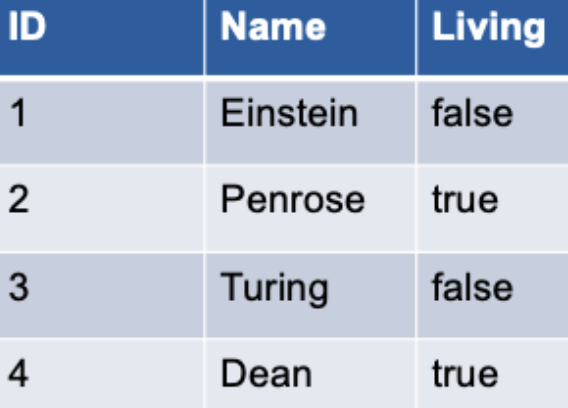
\includegraphics[width=0.6\textwidth]{Figures/FlatHomogeneous.png}
    \caption{Homogeneous flat Table}
\end{figure}
\end{minipage}

\begin{minipage}{0.55\textwidth}
\vspace{1\baselineskip}
\begin{lstlisting}[style=json,caption={JSON Code for a homogeneous and nested table.}]
{
    "ID":1,
    "Profession": "Physicist",
    "People": [
        {"Name": "Einstein", "Living" : false},
        {"Name": "Penrose", "Living" : true}
    ]
}
{
    "ID":2,
    "Profession": "Computer Scientist",
    "People": [
        {"Name": "Turing", "Living" : false},
        {"Name": "Dean", "Living" : true}
    ]
}
\end{lstlisting}
\end{minipage}
\hfill
\begin{minipage}{0.45\textwidth}
\begin{figure}[H]
    \centering
    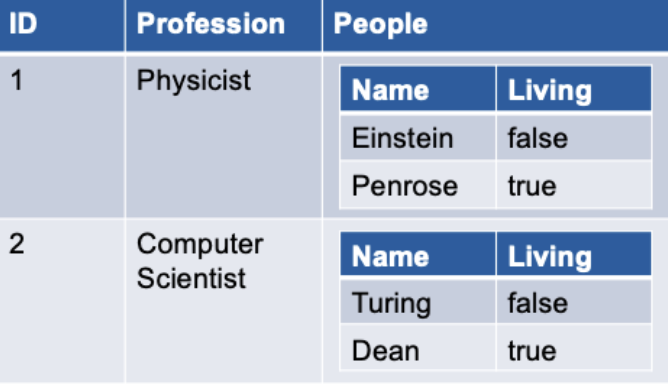
\includegraphics[width=0.9\textwidth]{Figures/NestedHomogeneous.png}
    \caption{Homogeneous nested Table}
\end{figure}
\end{minipage}


\begin{minipage}{0.55\textwidth}
\begin{lstlisting}[style=json,caption={JSON Code for a heterogeneous and flat table.}]
{
    "ID":1,
    "Name": "Einstein",
    "Living" : false,
    "Profession" : "Physicist"
}
{
    "ID":2,
    "Name": "Penrose",
    "Living" : true,
    "Profession" : "CS"
}
{
    "ID":3,
    "Name": "Turing"
}
{
    "ID":4,
    "Name": "Dean",
    "Living" : true
}
\end{lstlisting}
\end{minipage}
\hfill
\begin{minipage}{0.45\textwidth}
\begin{figure}[H]
    \centering
    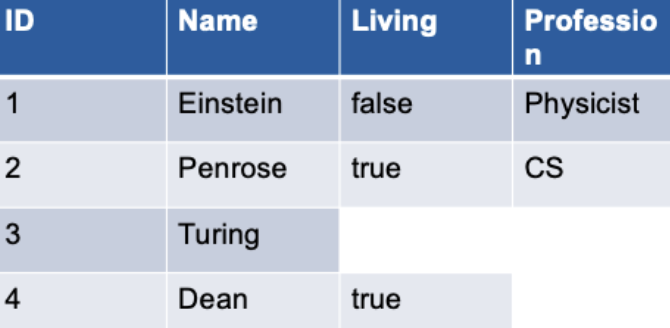
\includegraphics[width=0.9\textwidth]{Figures/FlatHeterogeneous.png}
    \caption{Heterogeneous flat Table}
\end{figure}
\end{minipage}


\begin{minipage}{0.55\textwidth}
\begin{lstlisting}[style=json,caption={JSON Code for a heterogeneous and nested table.}]
{
    "ID":1,
    "Profession": "Physicist",
    "People": [
        {"Name": "Einstein", "Living" : false},
        "Penrose"
    ]
} {
    "ID":2,
    "Profession": "Computer Scientist",
    "People": [
        {"Name": "Turing"},
        {"Name": "Dean", "Living" : true}
    ],
    "Comment": "They rock"
}
\end{lstlisting}
\end{minipage}
\hfill
\begin{minipage}{0.45\textwidth}
\begin{figure}[H]
    \centering
    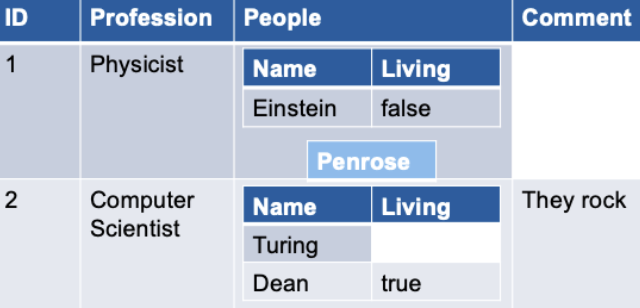
\includegraphics[width=0.9\textwidth]{Figures/NestedHeterogeneous.png}
    \caption{Heterogeneous nested Table}
\end{figure}
\end{minipage}


If the data is structured as a (valid) data frame, then there are many, many different formats that it can be stored in, and in a way that is much more efficient than JSON. These formats are highly optimized and typically stored in binary form, for example Parquet, Avro, Root, Google's protocol buffers, etc. If you see a JSON dataset that you are able to validate against a (e.g., JSound) schema that is "dataframe friendly", then you are highly encouraged to immediately build this schema, and convert the dataset to, say, Parquet. This gives you two immediate advantages:
\begin{itemize}
    \item space effciency: the file will be considerably smaller, meaning you can fit much more data even on your local laptop and it is also faster to transfer to and from the cloud to share with others.
    \item performance effciency: the smaller binary file will be much faster to read from disk when you write queries. In fact, many optimizers are able to skip entire sections of the data based on the query (projecting away a column, etc), making it even faster than it already was.
\end{itemize}
Generally, data formats can be classified along three dimensions:
\begin{itemize}
    \item whether they require validity against a data frame compatible schema (Parquet, protocol buffers, etc.) or not (JSON, XML, YAML, etc.).
    \item whether they allow for nestedness (Parquet, etc.) or not (CSV).
    \item whether they are textual (CSV, XML, JSON, etc.) or binary (Parquet, etc.), even though typically, formats that require a schema will be binary because of the “performance free lunch.”
\end{itemize}


\pagebreak

\section{Massive Parallel Processing}

\subsection{An Illustrative Example}

The Goal is to count species of dogs. Assume there are 10 different dog breeds and 1000 dogs in total. In order to count all the dogs as fast as possible, we parallelize the task. In the following we list the steps:

\paragraph{The Map}
Distribute all the 1000 dogs among 25 rooms with one person in each room. Each one of these people counts the number of dogs of all breeds of dog in his or her room and creates a list.

\paragraph{The Shuffle}
In a next step, another 10 people will be assigned a specific breed of dog. When the people from the room have created a list with the count of the dog breeds, they cut their list into the dogbreeds and hand the count of that specific breed to the person assigned that breed. 

\paragraph{The Reduce}
Lastly, the people who were assigned a specific dog breed then add together the count of their breed from the lists of all the rooms.

\paragraph{The Output}
When the number of all breeds of dogs have been calculated, they are merged together into one table.


\subsection{Patterns of large-scale query processing}

\subsubsection{Textual Input}

There are several different types of textual Inputs. These include:

\begin{itemize}
    \item Text: Billions of lines of texts
    \item CSV: plenty of CSV lines e.g.:
    
         \texttt{Year,Data,Duration,Guest}

         \texttt{2022,2019-04-25,00:37:59,UR}
    \item Use-case-specific textual format: e.g. \texttt{20222019-04-2500:37:59UR}
    \item Key-value pattern: e.g. \texttt{2022  00:37.59.000000}
    \item JSON Lines format: more popular. One JSON object per line. e.g.
    
    \texttt{\textbraceleft "year": 2022, "date": "2022-04-25", "duration": "00:37:59", "canton": "UR"\textbraceright}
\end{itemize}

\subsubsection{Other Input Formats}
Some other formats (e.g., Parquet, ...) can be binary or also HFiles.

\subsubsection{Shards}
How do we store Petabytes of data on online cloud storage, such as S3 or Azure blob storage, where the maximum size of a file is limited? Simply by spreading the data over many files. It is very common to have datasets lying in a directory spread over 100 or 1,000 files. Often, these files are named incrementally: part-0001, part-0002, etc. These files are often also called “shards” of the dataset.

Technically, HDFS would make it possible to have a gigantic, single file, automatically partitioned into blocks. However, also for HDFS, it is common to have a pattern with a directory containing many files named incrementally. The size of these files is typically higher than that of a block, for example 10 GB files.

Note that the size of the files do not constrain parallelism: with HDFS, even with 10 GB files, the 128 MB blocks within the same file can still be processed in parallel. S3 is also compatible with intra-file parallelism. There are several practical motivations for the many-files pattern even in HDFS:

\begin{itemize}
    \item It is much more convenient to output several shards from a framework like MapReduce than it is to create a single, big final file (which would require a way to concatenate it properly).
    \item It is considerably easier to download or upload datasets that are stored as many files. This is because network issues happen once in a while, and you can simply retry with only the files that failed.
\end{itemize}

\subsubsection{Querying Pattern}
Now that we have the data, how does querying it look like? On the very high-level, it converts some input to some output. However, because the underlying storage supports parallelism (via shards, blocks, regions, etc), the input as well as the output are partitioned. Ideally, the query could be reexpressed equivalently to simply map every input partition to an output partition. However, what you might find in reality is that the mapping is very chaotic and looks like a spaghetti from the input to the output. This is because there may be dependencies on several input partitions in an output partition. Fortunately, what happens often is somewhere in the middle, with some data flow patterns. Some places have data flowing in parallel (map-like) while some others are more spaghetti-y (shuffle-like).

This is the motivation behind the standard MapReduce pattern: a map-like phase on the entire input, then a shuffle phase on the intermediate data, then another map-like phase (called reduce) producing the entire output:

\begin{figure}[h]
    \centering
    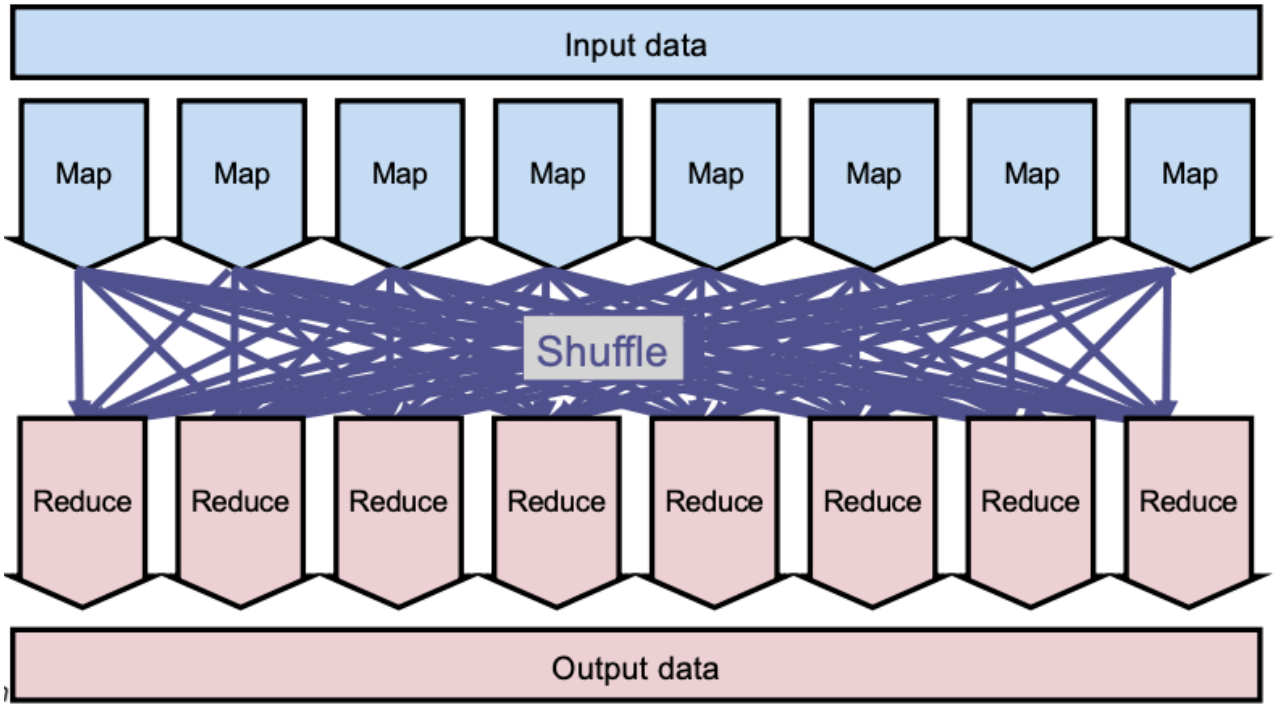
\includegraphics[width=0.6\textwidth]{Figures/StandardMapReduce.png}
    \caption{Standard Map Reduce}\label{fig:StdMapRed}
\end{figure}

\subsection{The MapReduce Model}

\subsubsection{Key-Value Pairs}
In MapReduce, the input data, intermediate data, and output data are all made of a large collection of key-value pairs (with the keys not necessarily unique, and not necessarily sorted by key). The types of the keys and values are known at compile-time (statically), and they do not need to be the same across all three collections. In practice, however, it is quite common that the type of the intermediate key-value pairs is the same as that of the output key-value pairs.

\subsubsection{Logical Walkthrough}
Everything starts with partitioning the input. MapReduce calls the partitions “splits”. Each key-value will be fed into a map function, mapping each value to a new intermediary key (e.g. from Key 1 of the input layer to Key \uproman{1} in the intermediate layer). However, as you can imagine, it would be extremely inefficient to do it pair by pair, thus, the map function is called in batches, on each split. Next, the new key-value pairs can be put together logically and logically sorted by their keys. Now, partition the table again, making sure the pairs with the same key are always in the same partition (but the partition can have pairs with several keys). The reduce function must then be called, for every unique key, on all the pairs with that key, outputting zero, one or more output pairs (in most cases it is one, and the key in the output layer is usually also the same as in the intermediate layer). Just like the map function, the reduce function is called in batches, on each intermediate partition (multiple calls, one per unique key). See \cref{fig:OverallMapRed} for a visual overview of the logical walkthrough of MapReduce.

\begin{figure}[h]
    \centering
    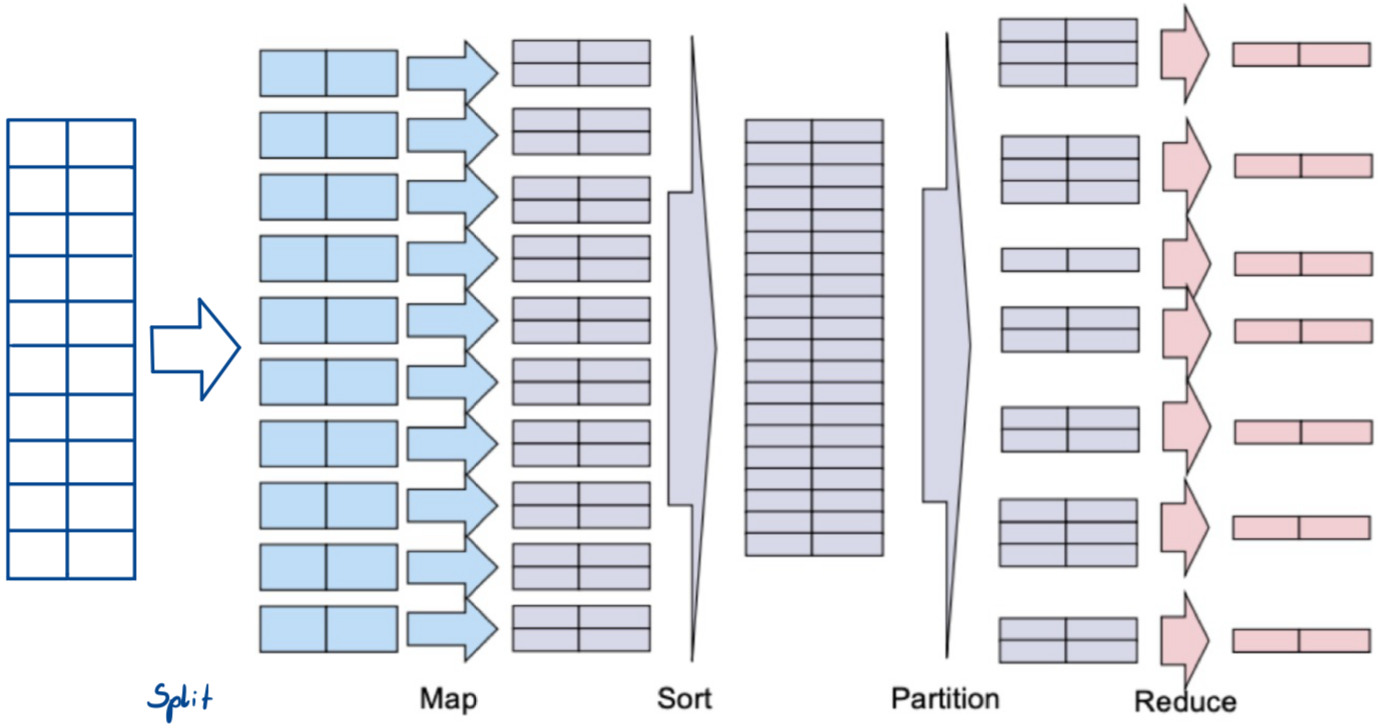
\includegraphics[width=0.9\textwidth]{Figures/OverallMapReduce.png}
    \caption{Overall MapReduce}\label{fig:OverallMapRed}
\end{figure}

\subsection{MapReduce Architecture}
MapReduce can read its input from many places as we saw: a cloud storage service, HDFS, a wide column store, etc. The data can be Petabyte-sized, with thousands of machines involved.

On a cluster, the architecture is centralized, just like for HDFS and HBase. In the original version of MapReduce, the main node is called JobTracker, and the worker nodes are called TaskTrackers. In fact, the JobTracker typically runs on the same machine as the NameNode (and HMaster) and the TaskTrackers on the same machines as the DataNodes (and RegionServers). This is called “bring the query to the data.” If using HDFS, then most of the time, for the map phase, things will be orchestrated in such a way that there is a replica of the block corresponding to the split on the same machine (since it is also a DataNode...), meaning that it is a local read and not a network connection.

As the map phase progresses, there is a risk that the memory becomes full. But we have seen this before with HBase: the intermediate pairs on that machine are then sorted by key and flushed to the disk to a Sequence File. And as more flushes happen, these Sequence Files can be compacted to less of them, very similarly to HBase’s Log-Structured Merge Trees.

When the map phase is over, each TaskTracker runs an HTTP server listening for connections, so that they can connect to each other and ship the intermediate data over to create the intermediate partitions ensuring that the same keys are on the same machines. This is the phase called shuffling. Then, the reduce phase can start.

Note that shuffling can start before the map phase is over, but the reduce phase can only start after the map phase is over.

When the reduce phase is completed, each output partition will be output to a shard (as we saw, a file named incrementally) in the output destination (HDFS, S3, etc) and in the desired format.

\subsection{MapReduce Input and Output Formats}

\subsubsection{Impedance Mismatch}

As the reader will have noticed, MapReduce only reads and writes lists of key-value pairs, where keys may be duplicates and need not appear in order. However, the inputs we considered are not key-value pairs. So we need an additional mechanism that allows MapReduce to interpret this input as key-value pairs.

For tables, whereas relational or in a wide column stores, this is relatively easy: indeed, tables have primary keys, consisting of either a single column or multiple columns. Thus, each tuple can be interpreted as a key-value pair, where the key is the (sub)tuple containing all the values associated with columns that are part of the primary key, while the value is the (sub)tuple containing the values associated with all other columns.

A key-value-pair is then one row of the tabel. The first column corresponds to the key and the remaining columns to the values.

\subsubsection{Mapping Files to Pairs}

How do we read a (possibly huge) text file as a list of key-value pairs? The most natural way to do so is to turn each line of text in a key value pair: the value is the string corresponding to the entire line, while the key is an integer that expresses the position (as a number of characters), or offset, at which the line starts in the current file being read. A small variation consists in reading N lines at a time, mapping them to a single key-value. Another variation consists of treating a character (picked by the user) specially, as the separator between the key and the value (e.g. space, semicolon, etc.).


\subsection{Examples}

\subsubsection{Counting Words}

We can count the words within each line similar to our motivation example with the cats, by mapping each line key-value to several key-values, one per word and with a count of 1. This gives us our map function. The reduce function is then obtained by summing the values with the same key, and keeping the same key. The output will then consist of a list of unique key-values, with one key for each word, and the number of its occurrences as the associated value.

\subsubsection{Selecting}

Filtering the lines containint a specific word can easily be done by having a map function that outputs a subset of its input, based on some predicate provided by the user. Here we notice that the output of the map phase already gives us the desired result; we still need to provide a reduce function, which is taken trivially as the identity function. This is not unusual.

In fact, what we have just implemented in MapReduce is nothing else than a selection operator from the relational algebra.

\subsubsection{Projecting}

What about projection on some input in the JSON Lines format? MapReduce doesn’t know anything about attributes. So it is up to the user to parse, in their code, each line to a JSON object (e.g., if using Python, to a dict). Then, the map function can project this object to an object with less attributes. Then, the map function can project this object to an object with less attributes. MapReduce will then output the results as one or several output files in the JSON Lines format.

\subsection{Combine Functions and Optimization}

In our counting example, we created an intermediate key-value for each occurrence of a word with a value set to 1. But what if a word appears 5 times on the same line? In this case, we can replace the corresponding key-value pairs with just one pair, with the value 5. Doing so is called combining and happens during the map phase.

Thus, in addition to the map function and the reduce function, the user can supply a combine function. This combine function can then be called by the system during the map phase as many times as it sees fit to “compress” the intermediate key-value pairs. Strategically, the combine function is likely to be called at every flush of key-value pairs to a Sequence File on disk, and at every compaction of several Sequence Files into one.

However, there is no guarantee that the combine function will be called at all, and there is also no guarantee on how many times it will be called. Thus, if the user provides a combine function, it is important that they think carefully about a combine function that does not affect the correctness of the output data. In fact, in most of the cases, the combine function will be identical to the reduce function, which is generally possible if the intermediate key-value pairs have the same type as the output key-value pairs, and the reduce function is both associative and commutative. This is the case for summing or multiplying values2 as well as for taking the maximum or the minimum, but not for an unweighted average. As a reminder, associativity means that $(a + b) + c = a + (b + c)$ and commutativity means that $a + b = b + a$.


\subsection{MapReduce Programming API}

In Java, the user needs to define a so-called Mapper class that contains the map function, and a Reducer class that contains the reduce function.

\subsubsection{Mapper Classes}
A map function takes in particular a key and a value. Note that it outputs key-value pairs via the call of the write method on the context, rather than with a return statement. That way, it can output zero, one or more key-values. A Mapper class looks like so:

\begin{lstlisting}[style=Java]
import org.apache.hadoop.mapreduce.Mapper;
public class MyOwnMapper extends Mapper<K1, V1, K2, V2>{
  public void map(K1 key, V1 value, Context context)
        throws IOException, InterruptedException
    {
        ...
        K2 new-key = ...
        V2 new-value = ... context.write(new-key, new-value); ...
    }
}
\end{lstlisting}

\subsubsection{Reducer Classes}

A reduce function takes in particular a key and a list of values. Note that it outputs key-value pairs via the call of the write method on the context, rather than with a return statement. That way, it can output zero, one or more key-values. A Reducer class looks like so:

\begin{lstlisting}[style=Java]
import org.apache.hadoop.mapreduce.Reducer;
public class MyOwnReducer extends Reducer<K2, V2, K3, V3> {
public void reduce (
        K2 key,
        Iterable<V2> values,
        Context context)
    throws IOException, InterruptedException
    {
        ...
        K3 new-key = ...
        V3 new-value = ... context.write(new-key, new-value); ...
    }
}
\end{lstlisting}

\subsection{Using Correct Terminology}

Let us now have a word of warning: the terminology “Mapper” and “Reducer” should only be used in the context of naming classes and files, but never when describing the MapReduce architecture. Even less so with “Combiner.”

\subsubsection{Functions}

\begin{itemize}
    \item A map function is a mathematical, or programmed, function that takes one input key-value pair and returns zero, one or more intermediate key-value pairs.
    \item A reduce function is a mathematical, or programmed, function that takes one or more intermediate key-value pairs (with the same key) and returns zero, one or more output key-value pairs.
    \item A combine function is a mathematical, or programmed, function that takes one or more intermediate key-value pairs (with the same key) and returns zero, one or more intermediate key-value pairs.
\end{itemize}

\subsubsection{Tasks}

\begin{itemize}
    \item Then, a map task is an assignment that consists in a (sequential) series of calls of the map function on a subset of the input. There is one map task for every input split, so that there are as many map tasks as partitions of the input.
    \item A reduce task is an assignment that consists in a (sequential) series of calls of the reduce function on a subset of the intermediate input. There are as many reduce tasks as partitions of the list of intermediate key-value pairs.
\end{itemize}

We insist that the calls within a task are sequential, meaning that there is no parallelism at all within a task. You can think of it as a for loop calling the function repeatedly, with the size of the for loop being, in a typical setting, between 1,000 and 1,000,000 calls.

There is no such thing as a combine task. Calls of the combine function are not planned as a task, but is called ad-hoc during flushing and compaction.

\subsubsection{Slots}

The map tasks are processed thanks to compute and memory resources (CPU and RAM). These resources are called map slots. One map slot corresponds to one CPU core and some allocated memory. The number of map slots is limited by the number of available cores. Each map slot then processes one map task at a time, sequentially. This means that the same map slot can process several map tasks.

The resources used to process reduce tasks are called reduce slots. Again, one reduce slot corresponds to one CPU core and some allocated memory. The number of reduce slots is limited by the number of available cores. Each reduce slot then processes one reduce task at a time, sequentially. This means that the same reduce slot can process multiple reduce tasks.

So, there is no parallelism either within one map slot, or one reduce slot. In fact, parallelism happens across several slots. In a typical MapReduce job, there will be more tasks than slots. Initially, each slot will receive one task, and the other tasks are kept pending. Every time a slot is done processing a task, it receives a new task from the pending list, and so on, until no task is left: then, some slots will remain idle until all tasks have been processed. If a task fails, it can be reassigned to another slot.

\subsubsection{Phases}

The map phase thus consists of several map slots processing map tasks in parallel and the reduce phase consists of several reduce slots processing reduce tasks in parallel. This is a summary of how functions, tasks, slots and phases fit together and within cluster nodes:

\begin{figure}[h]
    \centering
    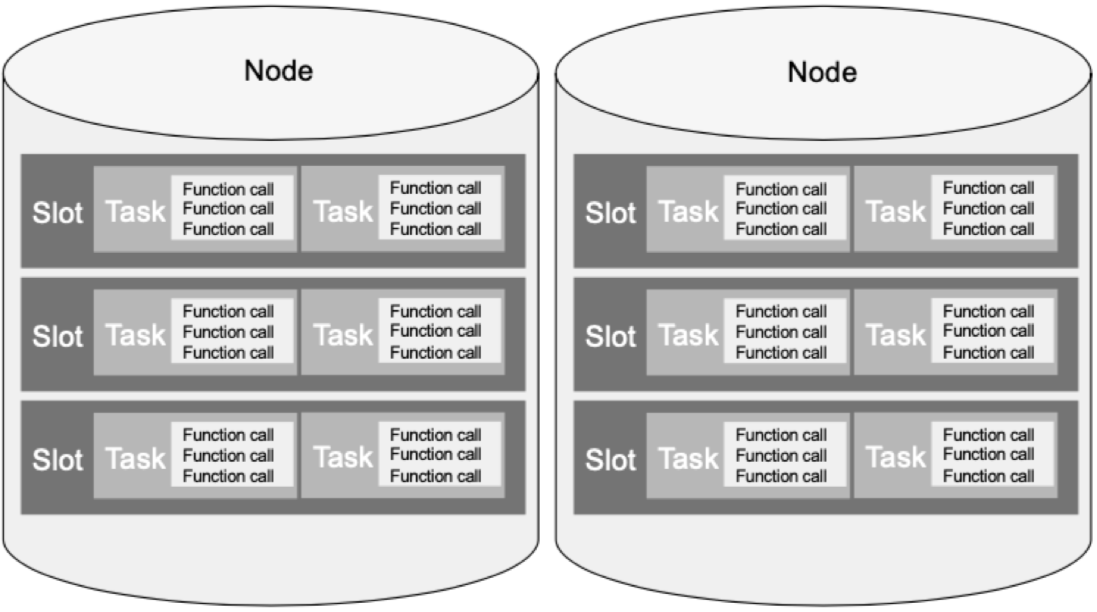
\includegraphics[width=0.7\textwidth]{Figures/MapReduceNodes.png}
    \caption{Summary of how functions, tasks and phases fit together and within cluster nodes.}
\end{figure}

\subsection{Impedance Mismatch: Blocks vs. Splits}
HDFS blocks have a size of (at most) 128 MB. In every file, all blocks but the last one have a size of exactly 128 MB. Splits, however, only contain full records: a key-value pair will only belong to one split (and thus be processed by one map task). This means that, while most key-value pairs will be in the same block, the first and/or last key-value pair in a split will be spread across two blocks. This means that, while most of the data is obtained locally, getting the first and/or last record in full will require a remote read over the HDFS protocol. This, in turn, is also the reason why the HDFS API gives the ability to only read a block partially.

\pagebreak

\section{Resource Management (Spark)}
In the very first version of MapReduce (with a JobTracker and TaskTrackers), map slots and reduce slots are all pre-allocated from the very beginning, which blocks parts of the cluster remaining idle in both phases. For this reason, the architecture was fundamentally changed by adding a resource management layer to the stack, adding one more level of decoupling between scheduling and monitoring. A resource management system, here YARN, is a very important building block not only for a better MapReduce, but also for many other technologies running on a cluster.

\subsection{Limitations of MapReduce in its First Version}
The JobTracker has a lot on its shoulders! It has to deal with resource management, scheduling, monitoring, the job lifecycle, and fault tolerance.
The first consequence of this is scalability: things start breaking beyond 4,000 nodes and/or 40,000 tasks.
The second consequence is the bottleneck that this introduces at the JobTracker level, which slows down the entire system.
The third issue is that it is diffcult to design a system that do many things well: “Jack of all trades, master of none”.
The fourth issue is that resources are statically allocated to the Map or the Reduce phase, meaning that parts of the cluster remain idle during both phases.
The fifth issue is the lack of fungibility between the Map phase and the Reduce phase: the system is closely tied to the two-phase mechanism of MapReduce, in spite of these two phases having a lot in common in terms of parallel execution.

\subsection{YARN}

\subsubsection{General Architecture}

YARN means Yet Another Resource manager. It was introduced as an additional layer that specifically handles the management of CPU and memory resources in the cluster.
YARN, is based on a centralized architecture in which the coordinator node is called the ResourceManager, and the worker nodes are called NodeManagers. NodeManagers furthermore provide slots (equipped with exclusively allocated CPU and memory) known as containers.

YARN provides generic support for allocating resources to any application and is application-agnostic. When the user launches a new application, the ResourceManager assigns one of the container to act as the ApplicationMaster which will take care of running the application. This is a fundamental change from the initial MapReduce architecture, in which the JobTracker was also taking care of running the MapReduce job. The ApplicationMaster can then communicate with the ResourceManager in order to book and use more containers in order to run jobs.

\begin{figure}[h]
    \centering
    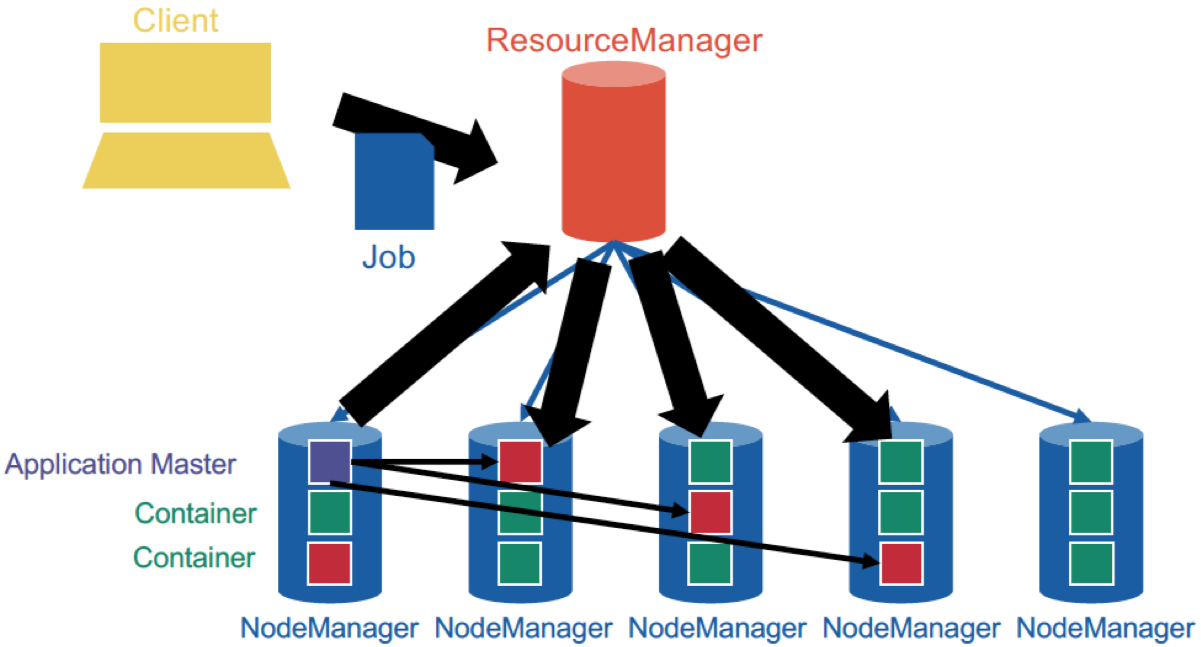
\includegraphics[width=0.7\textwidth]{Figures/YARNArchitecture.png}
    \caption{YARN Architecture}\label{fig:YARNArch}
\end{figure}

Thus, YARN cleanly separates between the general management of resources and bootstrapping new applications, which remains centralized on the coordinator node, and monitoring the job lifecycle, which is now delegated to one or more ApplicationMasters running concurrently. This means, in particular, that several applications can run concurrently in the same cluster.

\subsubsection{Resource Management}
There are four specific resources used in a distributed database system: Memory, CPU, Disk I/O and Network I/O. Most resource management systems (e.g. YARN) focus mainly on allocating and sharing memory and CPU.

ApplicationMasters can request and release containers at any time, dynamically. A container request is typically made by the ApplicationMasters with a specific demand. If the request is granted by the ResourceManager fully or partially, this is done indirectly by signing and issuing a container token to the ApplicationMaster that acts as proof that the resource was granted.

The ApplicationMaster can then connect to the allocated NodeManager and send the token. The NodeManager will then check the validity of the token and provide the memory and CPU granted by the ResourceManager. The ApplicationMaster ships the code (e.g., as a jar file) as well as parameters, which then runs as a process with exclusive use of this memory and CPU.

To bootstrap a new application, the ResourceManager can also issue application tokens to external clients so they can start the Application- Master.

There are as many ApplicationMasters as jobs. But only one resource manager. The ResourceManager does not monitor tasks and it does not restart upon failure.

The ApplicationMaster is application-specific. YARN is fully agnostic about the technology you are using.

\subsubsection{Job Lifecycle Management and Fault Tolerance}

The ApplicationMaster requests containers for the Map phase, and sets these containers up to execute Map tasks. As soon as a container is done executing a Map task, the ApplicationMaster will assign a new Map task to this container from the remaining queue, until no Map tasks are left.

It's the job of the ApplicationMaster to monitor for a failed task, and relaunch it with another container.


\subsection{Scheduling Stragegies}

\subsubsection{FIFO Scheduling}
In FIFO (First In First Out) scheduling, there is one application at a time running on the entire cluster. When it is done, the next application runs again on the entire cluster, and so on.

\subsubsection{Capacity Scheduling}
In capacity scheduling, the resources of the cluster are partitioned into several sub-clusters of various sizes. Each one of these sub-clusters has its own queue of applications running in a FIFO fashion within this queue.

Capacity scheduling also exists in a more "dynamic flavour" in which, when a sub-cluster is not currently used, its resources can be temporarily lent to the other sub-clusters. This is also in the spirit of usage maximization, so that the company as a whole will not waste unused resources.

\subsubsection{Fair Scheduling}
Fair scheduling involves more complex algorithms that attempt to allocate resources in a way fair to all users of the cluster and based on the share they are normally entitled to.

Fair scheduling should be understood in a dynamic fashion: the cluster has, at any point in time, users from various departments running their applications. Applications are dynamically and regularly requesting many containers with specific memory and CPU requirements, and releasing them again. Thus, fair scheduling consists on making dynamic decisions regarding which requests get granted and which requests have to wait.

\textcolor{grey}{More detail on Fair Scheduling in the Script on pages 268 and 289.}


\subsection{Summary}
\begin{itemize}
    \item We separate between scheduling and monitoring. (Scheduling is done by the ResourceManager and monitoring is done by the ApplicationMaster.)
    \item It is scalable. We can process more data than with the first version of map reduce.
    \item It is well available. You don't block the cluster unnecessarily. You don't have the bottleneck of the JobTracker anymore.
    \item It is multi-tenent. Meaning: you can have many people using the same cluster at the same time.
\end{itemize}


\pagebreak

\section{Generic Dataflow Management}

\subsection{A More General Dataflow Model}

MapReduce consists fo a map phase, followed by shuffling, followed by a reduce phase. Because reduce and map are essentially doing the same, one could also say that MapReduce follows the schema Map$\rightarrow$Shuffle$\rightarrow$Map. One can abstract away the partition and consider the nput, intermediate input and output as blackboxes that these phases act on.

\subsection{Resilient Distributed Datasets}
The first idea behind generic dataflow processing is to allow the dataflow to be arranged in any distributed acyclic graph (DAG), like so:

\begin{figure}[h]
    \centering
    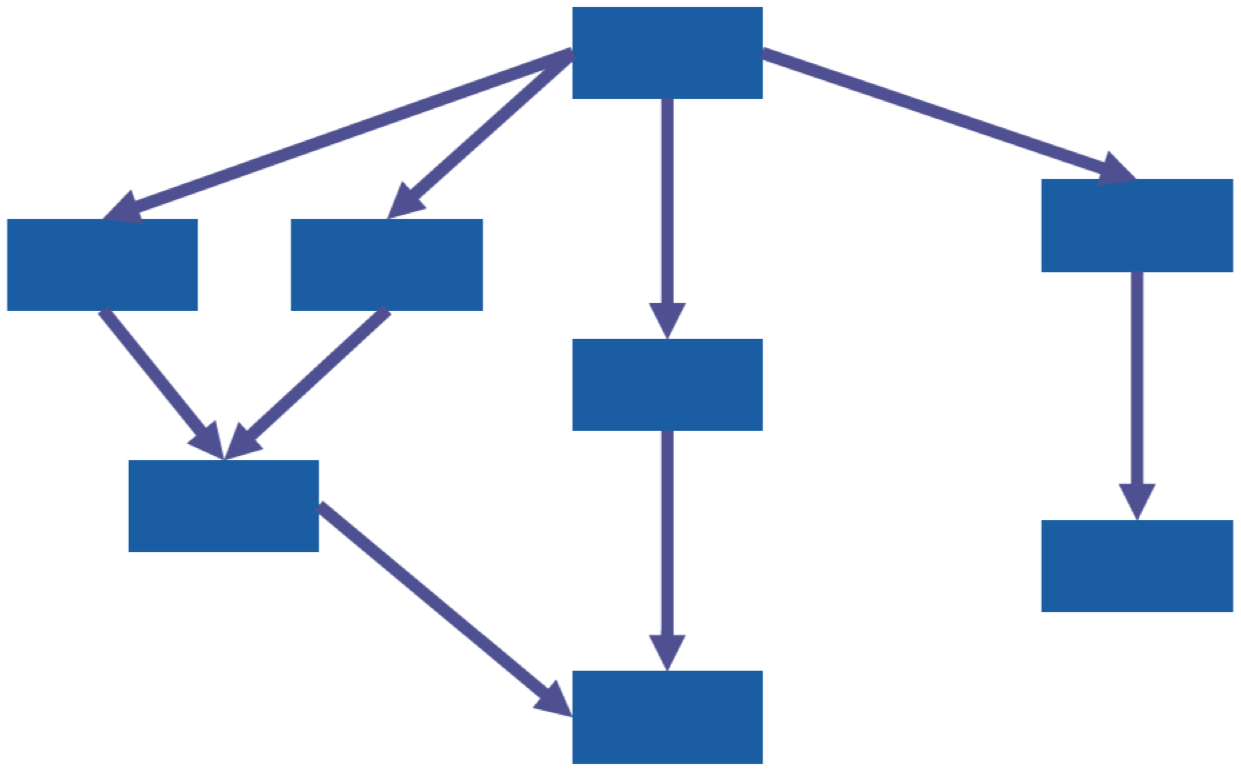
\includegraphics[width=0.4\textwidth]{Figures/DAGSpark.png}
    \caption{Dataflow in any DAG.}\label{fig:DAG}
\end{figure}

All the rectangular nodes in the above graph correspond to intermediate data. They are called resilient distributed datasets, or in short, RDDs. Resilient means that they remain in memory or on disk on a "best effort" basis, and can be recomputed if need be. Distributed means that, just like the collections of key-value pairs in MapReduce, they are partitioned and spread over multiple machines.

A major difference with MapReduce, though, is that RDDs need not be collections of pairs. In fact, RDDs can be (ordered) collections of just about anything. The only constraint is that the values within the same RDD share the same static type, which does not exclude the use of polymorphism.

Since a key-value pair is a particular example of possible value, RDDs are a generalization of the MapReduce model for input, intermediate input and output.


\subsection{The RDD Lifecycle}

\subsubsection{Creation}
RDDs can be created by reading a dataset from the local disk, or from cloud storage, or from a distributed file system, or from a database source, or directly on the fly from a list of values residing in the memory of the client using Apache Spark.

\subsubsection{Transformation}
RDDs can be transformed into other RDDs. Mapping or reducing, in this model, become two very specific cases of transformations. However, Spark allows for many more kinds of transformations. This also includes transformations with several RDDs as input (think of joins or unions in the relational algebra, for example).

\subsubsection{Action}
RDDs can also undergo a final action leading to making an output persistent. This can be by outputting the contents of an RDD to the local disk, to cloud storage, to a distributed file system, to a database system, or directly to the screen of the user.

\subsubsection{Lazy Evaluation}
The evaluation is lazy! Creations and transformations on their own do nothing. Only if an action is triggered, will the mappings like creations and transformations be computed. Especially, only those will be calculated that are needed for the action.


\subsection{Transformations}

\subsubsection{Unitary Transformations}

Unitary transformations are transformations that take only one RDD as their input.

\paragraph{Filter Transformation:} Provided a predicate function taking a value and returning a boolean, the Filter transformation returns the subset of its inputs that satisfy the predicate, preserving the relative order.

\paragraph{Map Transformation:} Provided a function taking a value and returning another value, the Map transformation returns the list of values obtained by applying this function to each value in the input.

\paragraph{flatMap Transformation:} Privided a function taking a value and returning zero, one or more values, the flatMap Transformation returns the list of values obtained by applying this function to each value in the input, flattening the obtained values (i.e. the information on which values came from the same input value is lost). The flatMap transformation corresponds to the MapReduce map phase.

\paragraph{Distinct Transformation} eliminates duplicates in the input. You either supply a comparison function, or you make sure that the class (type) of the input values implements the appropriate comparable interface.

\paragraph{Sample Transformation} samples the input to a smaller list. It is possible to specify the sampling percentage.


\subsubsection{Binary Transformations}

Binary transformations take two RDDs as inputs.

\paragraph{Union:} You concatenate two RDDs.

\paragraph{Intersection:} You filter the values that are present in both RDDs and create a new RDD out of these values.

\paragraph{Subtract:} Only keep the elements from the left RDD that do not appear in the right RDD.

\paragraph{Cartesian Product:} Looks for all possible combinations of the values in the left and right RDD and outputs pairs of these values. By default, Spark will not let you do this because it could yield enormous files.

\subsubsection{Pair Transformation}

\paragraph{key Transformation} returns a new RDD with only the keys.

\paragraph{value Transformation} returns a new RDD with only the values.

\paragraph{reduceByKey Transformation} given a binary operator, this function applies this function to all key values pairs with the same key. The reduceByKey transformation corresponds to the reduce phase of MapReduce.

\paragraph{groupByKey Transformation}  groups all key-value pairs by key, and outputs a single key-value for each key, where the value is an array (or list) of all the values that were associated with this key in the input.

\paragraph{sortByKey Transformation} given the specification of an order or comparison operator on the key type, the sortByKey transformation outputs the same pairs as in the input RDD, but reordered by key.

\paragraph{mapValues Transformation} similar to the map transformation, except that the map function is only applied to the value.

\paragraph{join Transformation} acts on two RDDs or key-value pairs. It matches pairs on both sides that have the same key and outputs, for each match, an ouput pair with that shared key and a tuple with the two valuse from each side. If there are multiple values with the same key on any side (or both), then all possible combinations are output.

\paragraph{subtractByKey:} outputs all pairs of the left, except those who have a key present on the right.


\subsection{Actions}

\subsubsection{Gathering output locally}

\paragraph{collect action} downloads all values of an RDD on the client machine and outputs them as a (local) list.

\paragraph{count action} computes (in parallel) the total number of values in the input RDD.

\paragraph{countByValue action} computes the total number of occurrence of each distinct value in the input RDD. The output is a python dictionary with the value as the key and the number of occurrences as the value.

\paragraph{take action} returns, as a local list, the first $n$ values in the input RDD.

\paragraph{top action} returns, as a local list, the last $n$ values from the input RDD.

\paragraph{takeSample action} returns, as a local list $n$ randomly picked values from the input RDD.

\paragraph{reduce action} given a (normally associative and commutative) binary operator, the reduce action invokes this operator on all values of the input RDD and outputs the resulting value.


\subsubsection{Actions on Pair RDDs}

(you can have repeating keys)

\paragraph{countByKey action} outputs, locally as a python dictionary, each key together with the number of values in the input that are associated with this key.

\paragraph{lookup action} outputs, locally, the value or values associated with a specific key.


\subsection{Physical Architecture}

There are two kinds of transformations: narrow-dependency transformations (not spaghetti-y) and wide-dependency transformations (spaghetti-y).

\subsubsection{Narrow-dependency Transformations}
Here, the computations of each output value involves a single input value. Thus, it is comparable to the map phase of MapReduce, and is easily parellelizable. Per default, there is one task per HDFS block.

The sequential calls of the transformation function on each input value within a single partitoin is called a task. Just like MapReduce, the tasks are assigned to slots. These slots correspond to cores within YARN containers. YARN containers used by Spark are called executors. The processing of the tasks is sequential within each executor, and tasks are executed in parallel across executors. A queue of unprocessed tasks is maintained, and everytime a slot is done, it gets a new task. When all tasks have been assigned, the slots who are done become idle and wait for all others to complete.

\subsubsection{Chains of narrow-dependency Transformations}

Consider the case of a chain of several narrow-dependency transformations, executed in turn (\cref{subfig:NDchain}). Naively, one could expect the execution to look like \cref{subfig:NaiveEx}. However, this would be very ineffienent because it requires shipping intermediate data over the network. But if all transformations are narrow-dependency transformations, it is possible to chain them without having data leaving the machines (\cref{subfig:EffEx}).

In fact, on the physical level, the physical calls of the underlying map/filter/etc functions are directly chained on each input value to directly produce the corresponding final, output value, meaning that the intermediate RDDs are not even materialized anywhere and exist purely logically. This means in particular that there is a single set of tasks, one for each partition of the input, for the entire chain of transformations. (\cref{subfig:BetterNDChain})

Such a chain of narrow-dependency transformations executed efficiently as a single set of tasks is called a stage, which would correspond to what is called a phase in MapReduce.

\begin{figure}[h]
    \centering
    \begin{subfigure}{0.47\textwidth}
        \centering
        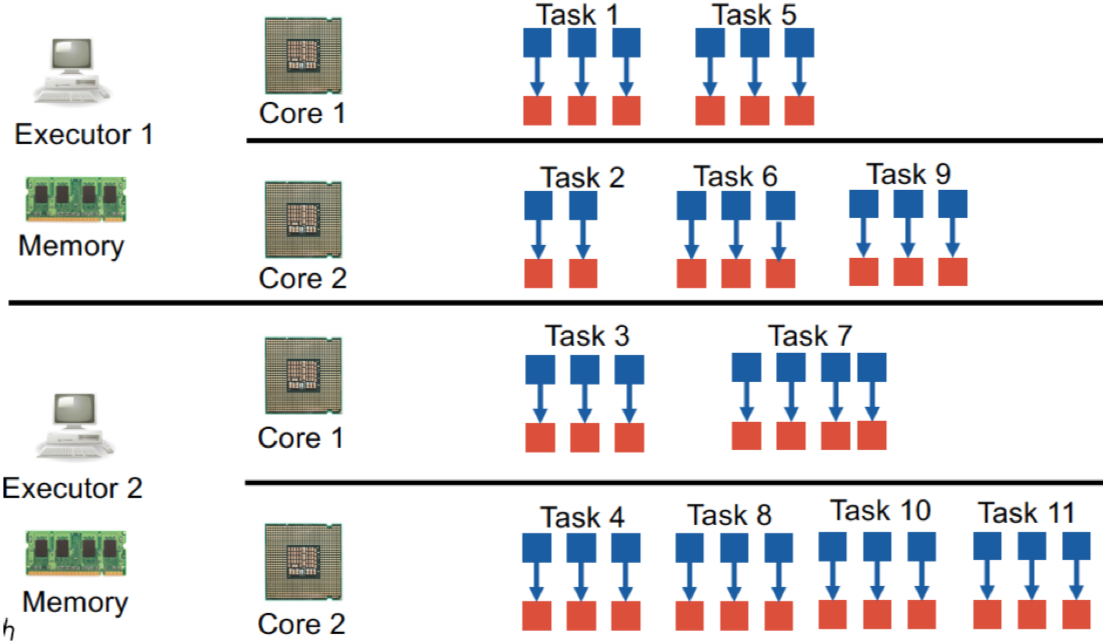
\includegraphics[width=\textwidth]{Figures/ChainTransformations.jpeg}
        \caption{Chain of several narrow-dependency transformations.}\label{subfig:NDchain}
    \end{subfigure}
    \hfill
    \begin{subfigure}{0.47\textwidth}
        \centering
        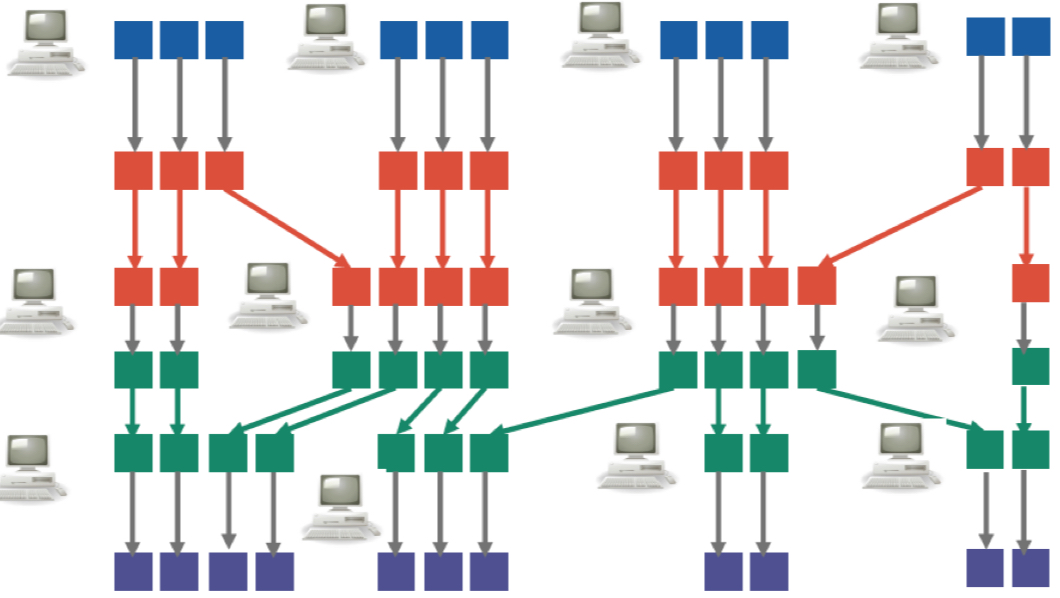
\includegraphics[width=\textwidth]{Figures/NaiveExecutionChain.jpeg}
        \caption{Naive Execution.}\label{subfig:NaiveEx}
    \end{subfigure}
    \begin{subfigure}{0.47\textwidth}
        \centering
        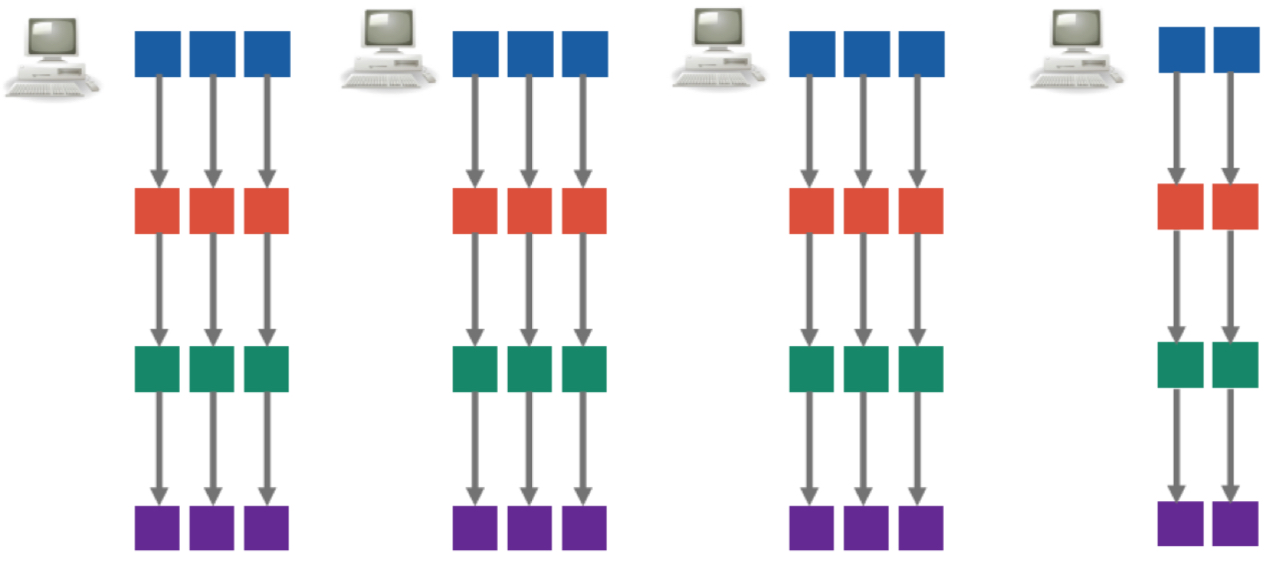
\includegraphics[width=\textwidth]{Figures/EfficientExecutionChain.jpeg}
        \caption{Efficient Execution.}\label{subfig:EffEx}
    \end{subfigure}
    \hfill
    \begin{subfigure}{0.47\textwidth}
        \centering
        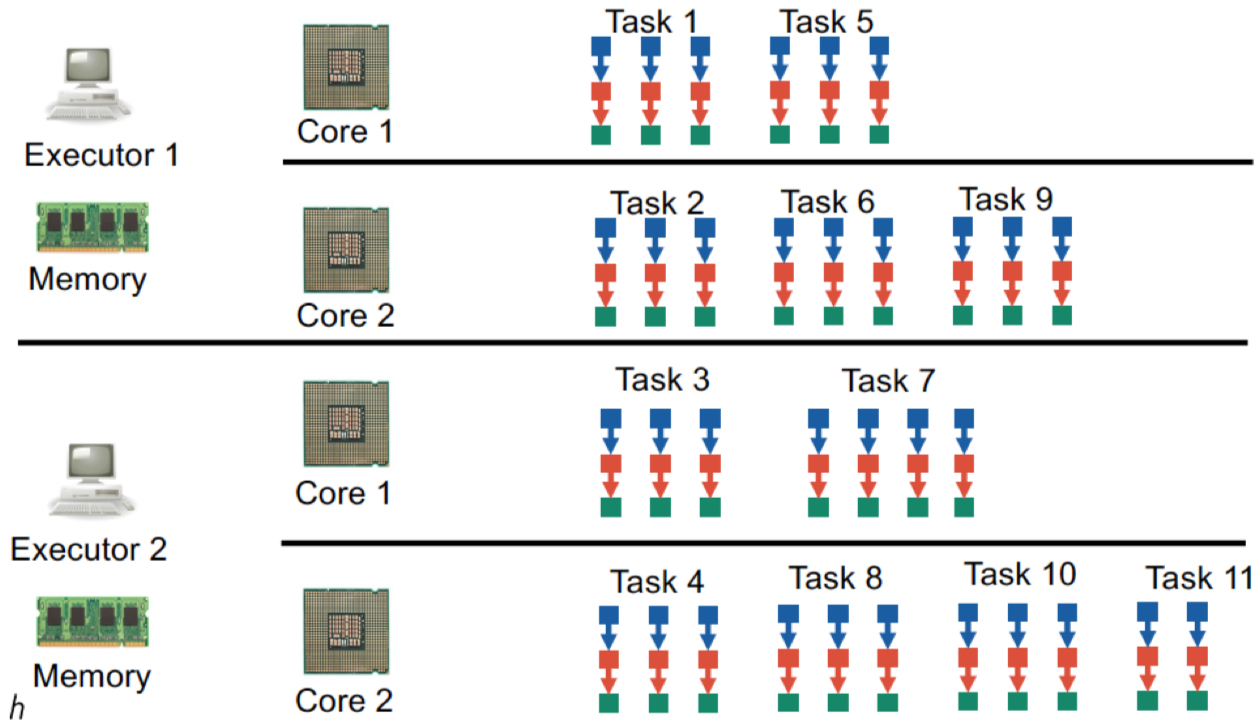
\includegraphics[width=\textwidth]{Figures/BetterNDChain.jpeg}
        \caption{Parallelized Executions.}\label{subfig:BetterNDChain}
    \end{subfigure}
    \caption{Narrow-dependency Transformations}\label{fig:NDTransfo}
\end{figure}

\subsubsection{Physical Parameters}
Users can parameterize how many executors there are, how many cores there are per executor and how much memory per executor. E.g.

\begin{lstlisting}[style=Java]
spark-submit
    --num-executors 42
    --executor-cores 2
    --executor-memory 3G
    my-application.jar
\end{lstlisting}

\subsubsection{Shuffling}
Wide-dependency transformations involve a shuffling of the data over the network, so that the data necessary to compute each partition of the output RDD is physically at the same location. Thus, on the high-level of a job, the physical execution consists of a sequence of stages, with shuffling happening everytime a new stage begins (\cref{subfig:stageshuffleseq})

Even though one can imagine a physical implementation in which two stages are executed at the same time on two sub-parts of the cluster, a more typical setting is a linear succession of stages on the physical level. (\cref{subfig:parallStageShuffleSeq})

\begin{figure}[h]
    \centering
    \begin{subfigure}{0.47\textwidth}
        \centering
        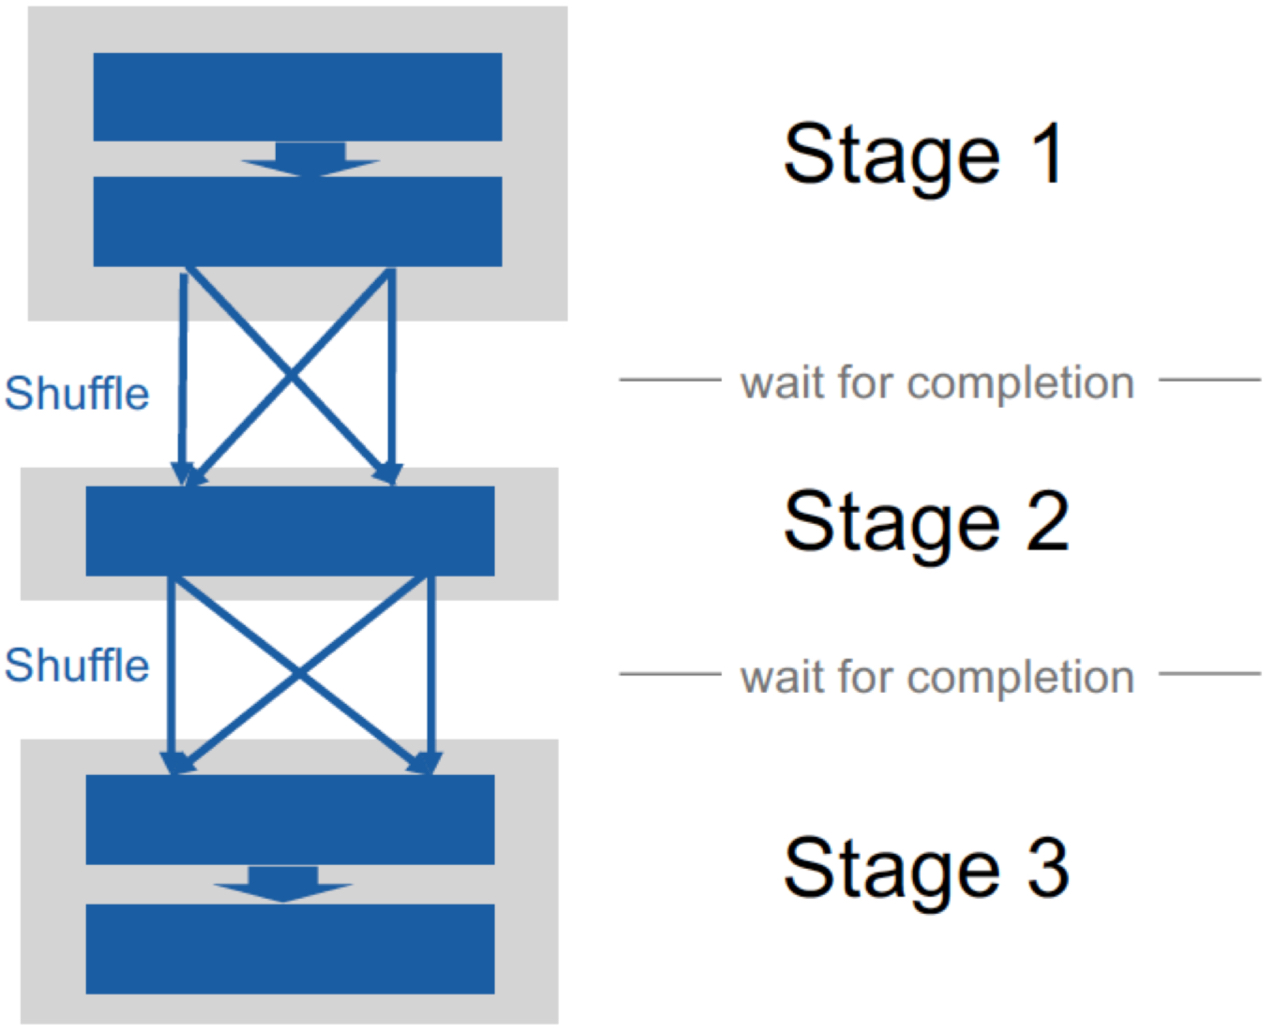
\includegraphics[width=0.8\textwidth]{Figures/StageShuffleSequence.jpeg}
        \caption{Sequence of Stages and Shuffles.}\label{subfig:stageshuffleseq}
    \end{subfigure}
    \hfill
    \begin{subfigure}{0.48\textwidth}
        \centering
        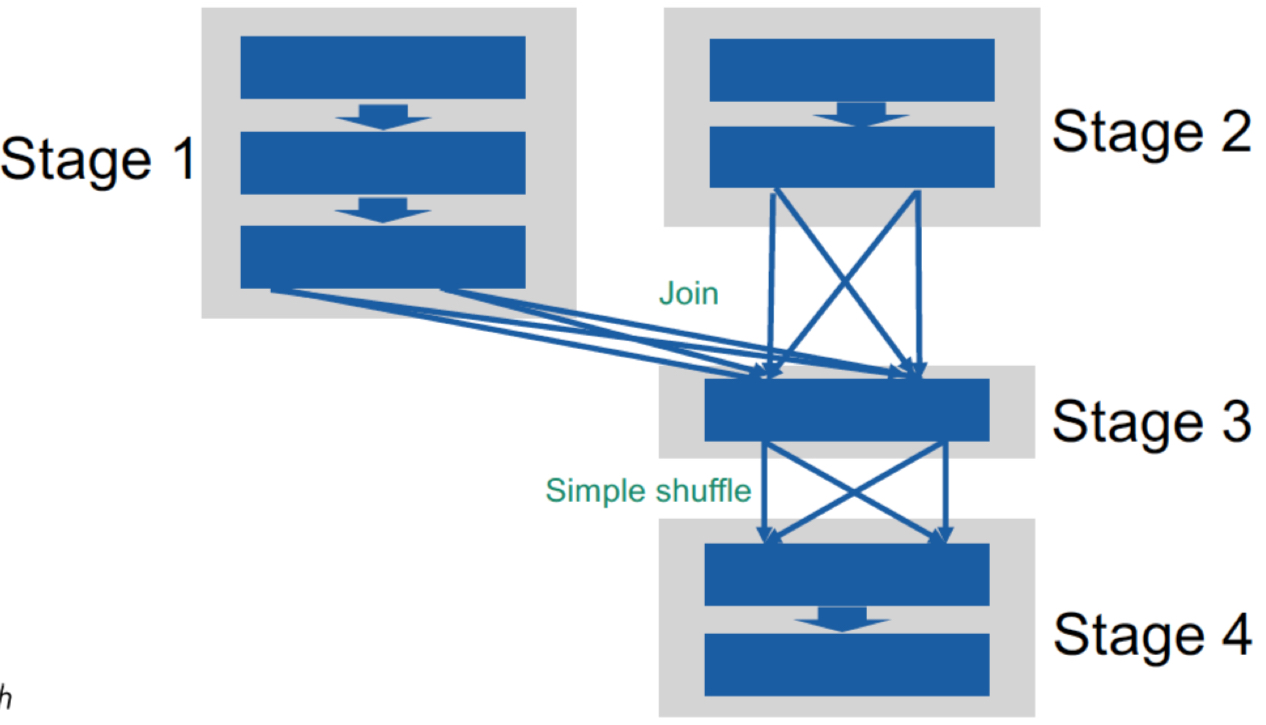
\includegraphics[width=\textwidth]{Figures/ParellelStageShuffleSeq.jpeg}
        \caption{Parallel Sequence of Stages and Shuffles.}\label{subfig:parallStageShuffleSeq}
    \end{subfigure}
    \caption{Sequence of Stages and Shuffles.}
\end{figure}

\subsubsection{Optimization}

\paragraph{Pinning RDDs}
In some cases, several actions might share subgraphs of the DAG. It makes sense, then, to “pin” the intermediate RDD by persisting it. It is possible to ask for persistence in memory and/or on disk.

\paragraph{Pre-Partitioning}
Shuffle is needed to bring together the data that is needed to jointly contribute to individual output values. If, however, Spark knows that the data is already located where it should be, then shuffling is not needed.

\subsubsection{Summary}
Tasks, Transformations, Stages and Jobs relate as can be seen in \cref{fig:Terminology}

\begin{figure}[h]
    \centering
    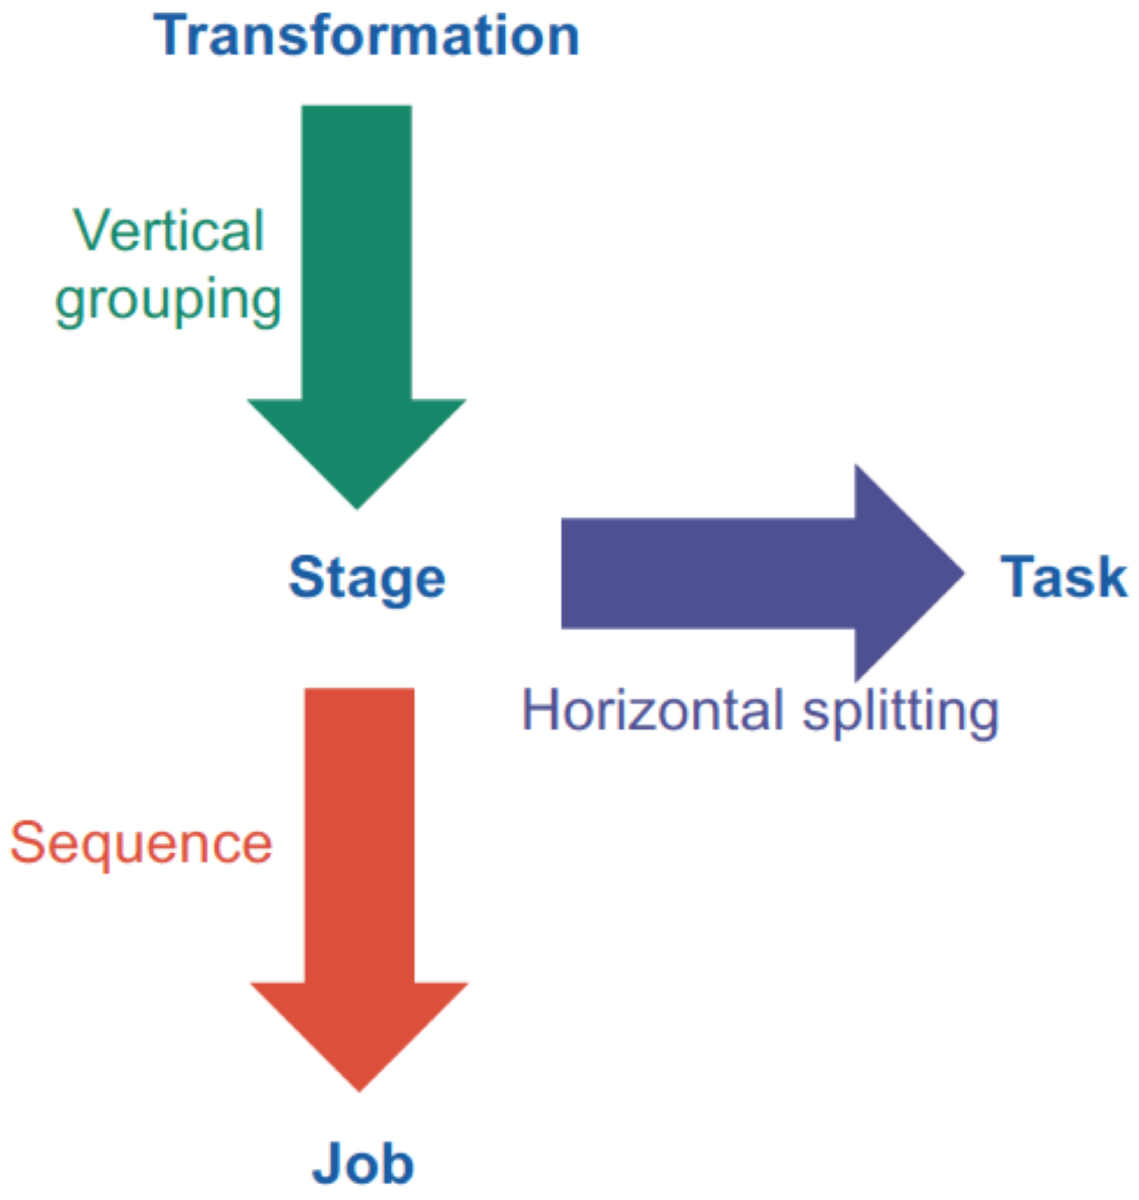
\includegraphics[width=0.4\textwidth]{Figures/Terminology.jpeg}
    \caption{Terminology}\label{fig:Terminology}
\end{figure}


\subsection{DataFrames in Spark}

\subsubsection{Data Independence}
Unlike a relational database that has everything right off-the-shelf, with RDDs, the user has to reimplement all the primitives they need.

\subsubsection{A Specific Kind of RDD}
A DataFrame can be seen as a specific kind of RDD: an RDD of rows (equivalently: tuples, records) that has relational integrity, domain integrity, but not necessarily atomic integrity. DataFrames can also be characterized as homogeneous collections of valid JSON objects (which are the rows) against a schema. It is thus only logical that, in Spark, every DataFrame has a schema.

The immediate consequence is that, in the particular case of flat rows, an RDD of (flat) rows is a relational table. Thus, it is very natural to think of SQL as the natural language to query them.

\subsubsection{Performance Impact}
DataFrames are not only useful because of the higher, more convenient, level of abstraction that they provide to the user, enhancing their productivity. DataFrames also have a positive impact on performance, because Spark can do a much better job of optimizing the memory footprint and the processing. In particular, DataFrames are stored column-wise in memory, meaning that the values that belong to the same column are stored together. Furthermore, since there is a known schema, the names of the attributes need not be repeated in every single row, as would be the case with raw RDDs. DataFrames are thus considerably more compact in memory than raw RDDs.

Generally, Spark converts Spark SQL to internal DataFrame transformation and eventually to a physical query plan. An optimizer known as Catalyst is then able to find many ways of making the execution faster, as knowing the DataFrame schema is invaluable information for an optimizer, as opposed to generic RDDs of which one knows little statically.

As an example, since the data is stored by columns, whenever Spark knows that some columns are not used by subsequent transformations and actions, it can silently drop these unused columns with no consequence. This is called “projecting away” and it is one of the most important optimizations in large-scale databases. Projecting away can even be done already at the disk level, i.e., when reading a Parquet file, it is possible to read only the columns that are actually needed, which significantly reduces the I/O bottleneck and accelerates the job.


\subsubsection{Input Formats}
Here an example of code in which a dataset is directly read as JSON. 

\begin{lstlisting}[style=neutral]
df = spark.read.json('hdfs:///dataset.json')
df.createOrReplaceTempView("dataset")
df2 = df.sql("SELECT * FROM dataset "
"WHERE guess = target "
"ORDER BY target ASC, country DESC, date DESC")
result = df2.take(10)
\end{lstlisting}

Note that Spark automatically infers the schema from discovering the JSON Lines file, which adds a static performance overhead that does not exist for raw RDDs. CSV also come with a schema discovery, although this one is optional (as by default, one can treat all values as strings). Builtin input formats can be specified, when creating a DataFrame from a dataset, with a simple method call after the read command. Non-builtin formats are supplied as a string parameter to a format() method. This is extensible and it is possible to “make” a format builtin via extension libraries.

\begin{lstlisting}[style=neutral]
df = spark.read.json("hdfs:///dataset.json")
df = spark.read.parquet("hdfs:///dataset.parquet")
df = spark.read.csv("hdfs:///dir/*.csv")
df = spark.read.text("hdfs:///dataset[0-7].txt")
df = spark.read.jdbc("jdbc:postgresql://localhost/test?user=fred&password=secret",...)
df = spark.read.format("avro").load("hdfs:///dataset.avro")
\end{lstlisting}

\subsubsection{DataFrame Column Types}
There are atomic (\cref{fig:AtomicTypes}) and structured types (\cref{fig:StructuredTypes}). As a reminder, structs have string keys and arbitrary value types and correspond to generic JSON objects, while in maps, all values have the same type. Thus, structs are more common than maps. Arrays correspond to JSON arrays.

\begin{figure}[h]
    \centering
    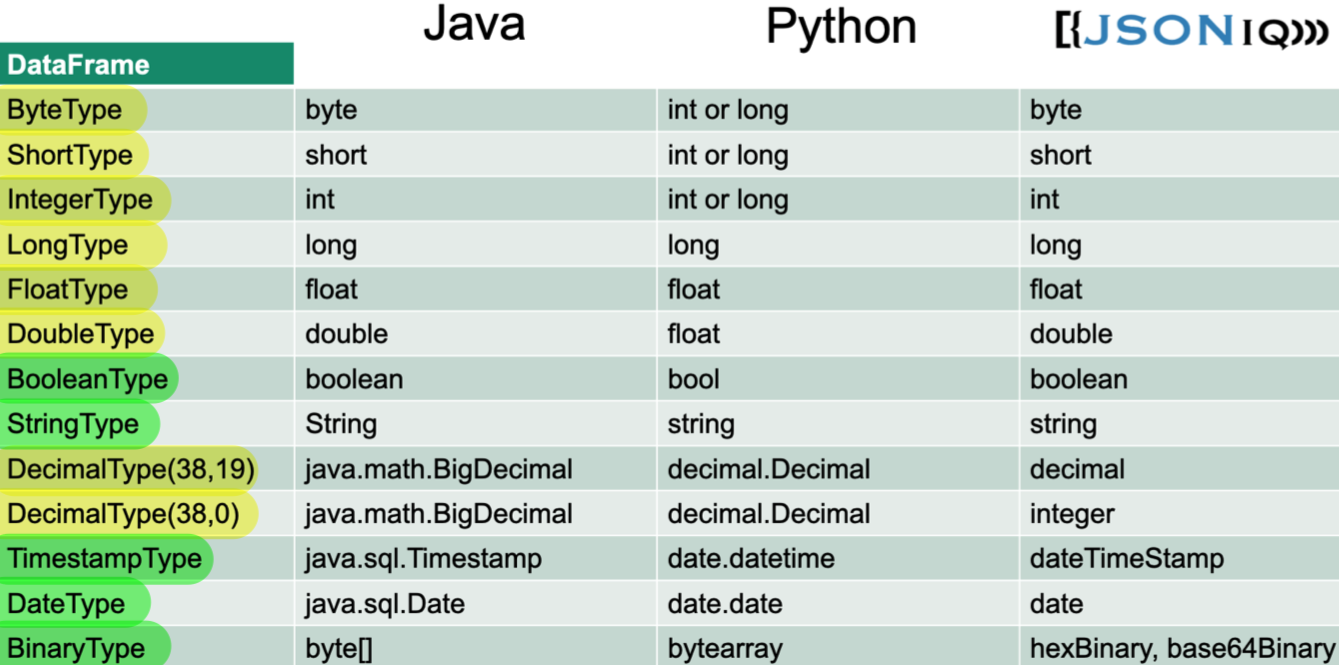
\includegraphics[width=0.8\textwidth]{Figures/DataFrameTypes.png}
    \caption{Atomic DataFrame Types. Yellow corresponds to Number types and green corresponds to non-number types (/other atomics)}\label{fig:AtomicTypes}
\end{figure}

\begin{figure}[h]
    \centering
    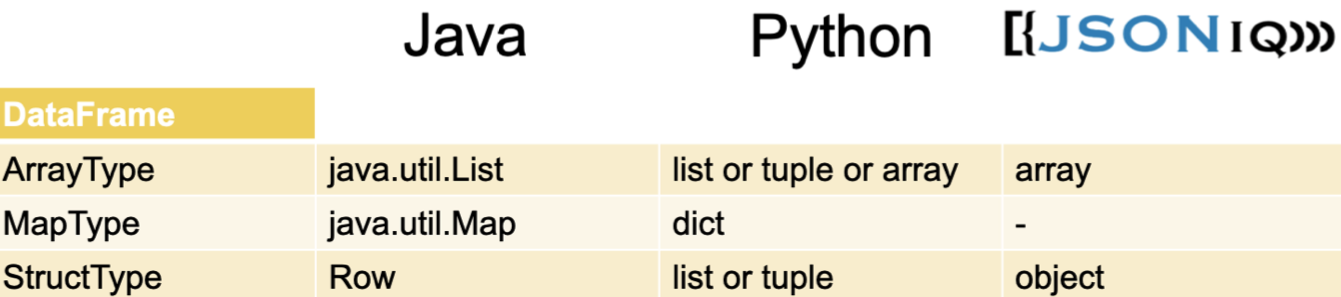
\includegraphics[width=0.7\textwidth]{Figures/DataFrameTypes2.png}
    \caption{Structured DataFrame Types.}\label{fig:StructuredTypes}
\end{figure}

\subsubsection{The Spark SQL Dialect}

We mentioned that Spark SQL is a dialect of SQL. Spark SQL has a few limitations (i.e., there is no OFFSET clause) but also comes with a few convenient extensions, in particular to deal with nested data.

\begin{lstlisting}[style=sql]
SELECT first_name, last_name
FROM persons
WHERE age >= 65
GROUP BY country
HAVING COUNT(*) >= 1000
ORDER BY country DESC NULLS FIRST
LIMIT 100
\end{lstlisting}

GROUP BY and ORDER BY will trigger a shuffle in the system, even though this can be optimized as the grouping key and the sorting key are the same.

The SORT BY clause can sort rows within each partition, but not across partitions, i.e., does not induce any shuffling.

The DISTRIBUTE BY clause forces a repartition by putting all rows with the same value (for the specified field(s)) into the same new partition.

\begin{minipage}{0.45\textwidth}
\begin{lstlisting}[style=sql]
SELECT first_name, last_name
FROM persons
WHERE age >= 65
GROUP BY country
HAVING COUNT(*) >= 1000
SORT BY country DESC NULLS FIRST
\end{lstlisting}
\end{minipage}
\hfill
\begin{minipage}{0.45\textwidth}
\begin{lstlisting}[style=sql]
SELECT first_name, last_name
FROM persons
WHERE age >= 65
GROUP BY country
HAVING COUNT(*) >= 1000
DISTRIBUTE BY country
\end{lstlisting}
\end{minipage}

It is possible to use both SORT and DISTRIBUTE, but this is equivalent to the use of another clause, CLUSTER BY:

\begin{minipage}{0.45\textwidth}
\begin{lstlisting}[style=sql]
SELECT first_name, last_name
FROM persons
WHERE age >= 65
GROUP BY country
HAVING COUNT(*) >= 1000
SORT BY country DESC NULLS FIRST
DISTRIBUTE BY country
\end{lstlisting}
\end{minipage}
\hfill
\begin{minipage}{0.45\textwidth}
\begin{lstlisting}[style=sql]
SELECT first_name, last_name
FROM persons
WHERE age >= 65
GROUP BY country
HAVING COUNT(*) >= 1000
CLUSTER BY country
\end{lstlisting}
\end{minipage}

Spark SQL also comes with language features to deal with nested arrays and objects.
First, nested arrays can be navigated with the explode() function, like so:

\begin{figure}[h]
    \centering
    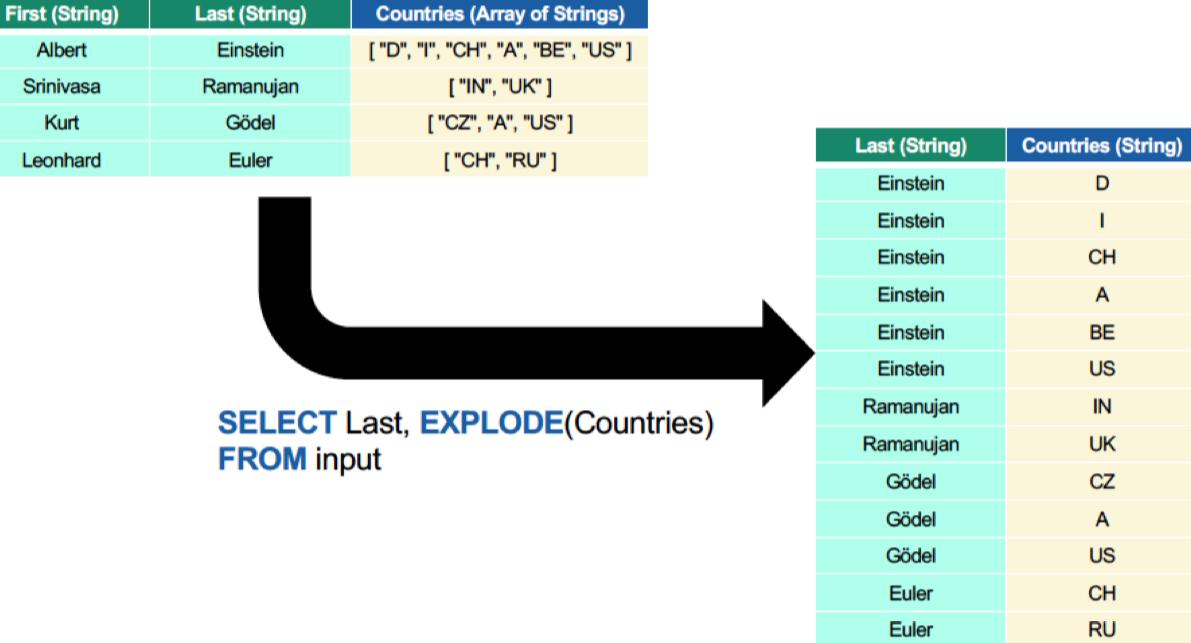
\includegraphics[width=0.8\textwidth]{Figures/Explode.png}
    \caption{Explode}\label{fig:Explode}
\end{figure}

Explode() cannot deal with all use cases, though, which is why there is another, more generic construct known as LATERAL VIEW. A lateral view can be intuitively described this way: the array mentioned in the LATERAL VIEW clause is turned into a second, virtual table with the rest of the original table is joined. The other clauses can then refer to columns in both the original and second, virtual table. This yields the same result as can be seen in \cref{fig:Explode}.  Lateral views are more powerful and generic than just an explode() because they give more control, and they can also be used to go down several levels of nesting, like in \cref{fig:LatView}.

\begin{figure}[h]
    \centering
    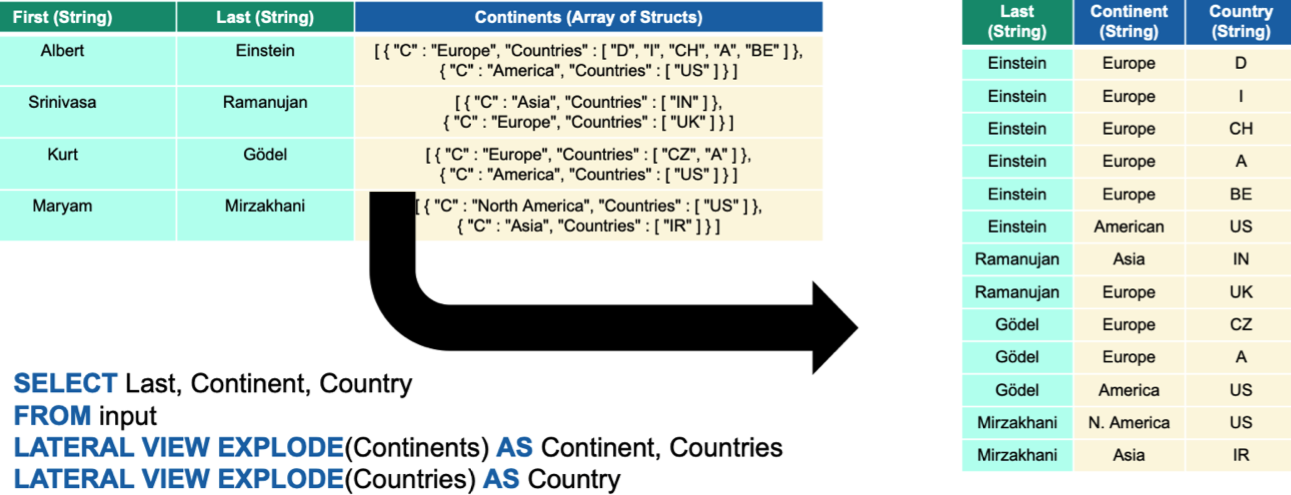
\includegraphics[width=0.8\textwidth]{Figures/LateralViewExplode.png}
    \caption{Lateral View}\label{fig:LatView}
\end{figure}

It is also possible to navigate and “unnest” nested structs (objects) using dots, like in \cref{fig:Unnest}.

\begin{figure}[h]
    \centering
    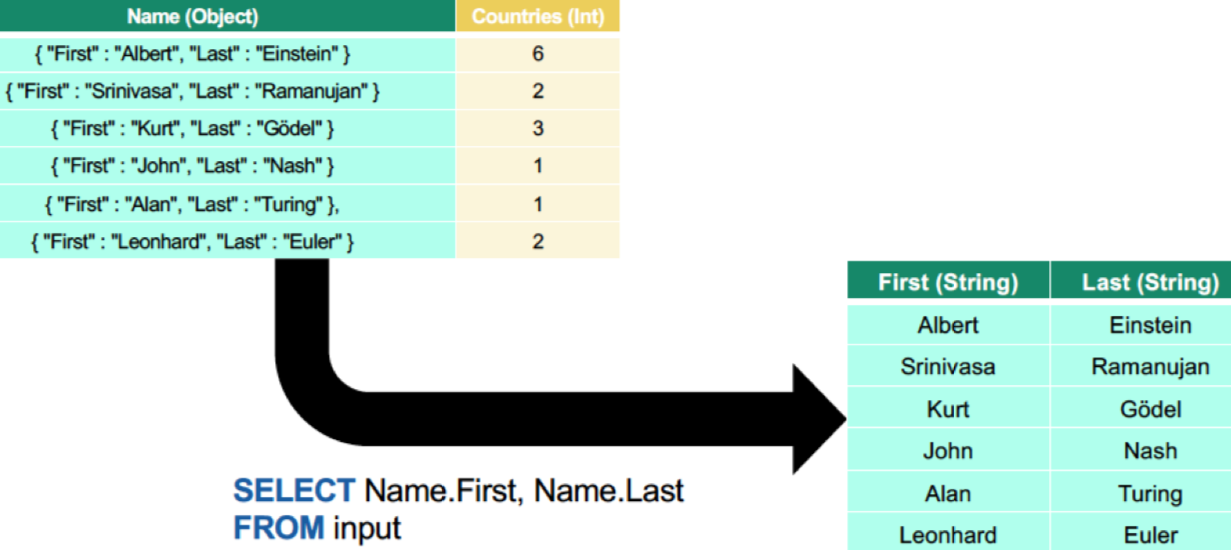
\includegraphics[width=0.8\textwidth]{Figures/UnnestStructs.png}
    \caption{Unnest nested structs.}\label{fig:Unnest}
\end{figure}

DataFrames and Spark SQL do support data that is not in first normal form, but they do not support at all data that does not fulfill relational integrity or domain integrity. It is possible to read as input a JSON Lines dataset with inconsistent value types in the same columns, however the schema discovery phase will simply result in a column with type “string”, which puts all the burden of dealing with the polymorphism of the column to the end user.


\subsubsection{DataFrames and RDDs}
Under the hood, when creating dataframes, spark is storing them as RDDs. But you can also do it explicitely. If you have a dataframe, you can force-convert it to an RDD and vice versa. But to turn an RDD into a dataframe, you need a schema. See \cref{lst:DFaRDD}.

\vspace{1\baselineskip}

\begin{lstlisting}[style=neutral,caption={DataFrames and RDDs},label={lst:DFaRDD}]
# Create an RDD file from a DataFrame
rdd = df.rdd

# Create a DataFrame from an RDD file
df = rdd.toDF()
# or
df = sc.createDataFrame(rdd,schema)
\end{lstlisting}


\pagebreak

\section{Document Stores}

A document store, unlike a data lake, manages the data directly and the users do not see the physical layout.
\textcolor{red}{You will not have to write MongoDB code in the Exam!}

\subsection{Relational Databases}
In relational databases, everything is a table. We saw that a table can be seen as a set of maps (from attributes to values) that fulfils three constraints: relational integrity, domain integrity, and atomic integrity. It can optimize the layout of the data on disk and build additional structures (indices) to accelerate SQL queries without the need
to modify them, and it can handle transactions.

\subsection{Challenges}

\subsubsection{Schema on read}
Data that fulfills relational integrity, domain integrity, and atomic integrity always comes with a schema. In a relational database management system, it is not possible to populate a table without having defined its schema first.

When encountering such denormalized data, in the real world, there is often no schema. In fact, one of the important features of a system that deals with denormalized data is the ability to discover a schema, i.e., offer query functionality to find out which keys appear in the data, what kind of value is associated with each key, etc; or even functionality that directly infers a schema, as we saw is the case with Apache Spark.

In Document stores, you can just pour your trees into your collection, without a schema, and it will just work, even if the trees are heterogeneous. But if you want a schema, you can have one. You can either define a schema from the very beginning, and then allow the documents that fit the schema and throw an error if they don't, or you can first pour your trees into your collection, then maxbe clean it up and then validate against the schema and then force the validation forever. Thus we are not obligated to check for a schema from the beginning, we can do it later.

\subsubsection{Making trees fit in tables}

A first thought when trying to build a system that supports denormalized data, such as collections of JSON or XML objects, is to force-fit it into tables. In fact, it is a very natural thing to do if the collection is flat and homogeneous, i.e., respects the three fundamental integrity constraints.

\vspace{1\baselineskip}

\begin{minipage}{0.26\textwidth}
\begin{lstlisting}[style=json,caption={JSON Object}]
{
    "foo":      1,
    "bar":      "foo",
    "foobar":   true,
    "a":        "bar",
    "b":        3.14
}
\end{lstlisting}
\end{minipage}
\hfill
\begin{minipage}{0.3\textwidth}
\begin{lstlisting}[style=xml,caption={XML Object}]
<row>
    <foo>1</foo>
    <bar>foo<\bar>
    <foobar>true</foobar>
    <a>foo</a>
    <b>3.14</b>
</row>
\end{lstlisting}
\end{minipage}
\hfill
\begin{minipage}{0.3\textwidth}
\begin{tabular}{c|c|c|c|c}
    foo & bar & foobar & a & b \\ \hline
    1 & foo & true & foo & 3.14
\end{tabular}
\end{minipage}

The corresponding XML Schemas can also be transformed naturally to a relational schema. The same goes for JSound or JSON Schemas.

\begin{lstlisting}[style=xml,caption={XML Schema}]
<xs:schama xmlns:xs="http://www.w3.org/2001/XMLSchema">
    <xs:element name="row">
        <xs:complexType>
            <xs:sequence>
                <xs:element name="foo" type="xs:integer"/>
                <xs:element name="bar" type="xs:string"/>
                <xs:element name="foobar" type="xs:boolean"/>
                <xs:element name="a" type="xs:string"/>
                <xs:element name="b" type="xs:decimal"/>
            </xs:sequence>
        </xs:complexType>
    </xs:element>
</xs:schema
\end{lstlisting}   

\begin{lstlisting}[style=json,caption={JSON Schema}]
{
  "foo"   :   "integer",
  "bar"   :   "string",
  "foobar":   "boolean",
  "a"     :   "string",
  "b"     :   "decimal"
}
\end{lstlisting}    

This however, is generally not a great approach because semi-structured data can be nested and heterogeneous. One possible way to deal with this issue may be:

\begin{figure}[h]
    \centering
    \begin{subfigure}{0.49\textwidth}
        \centering
        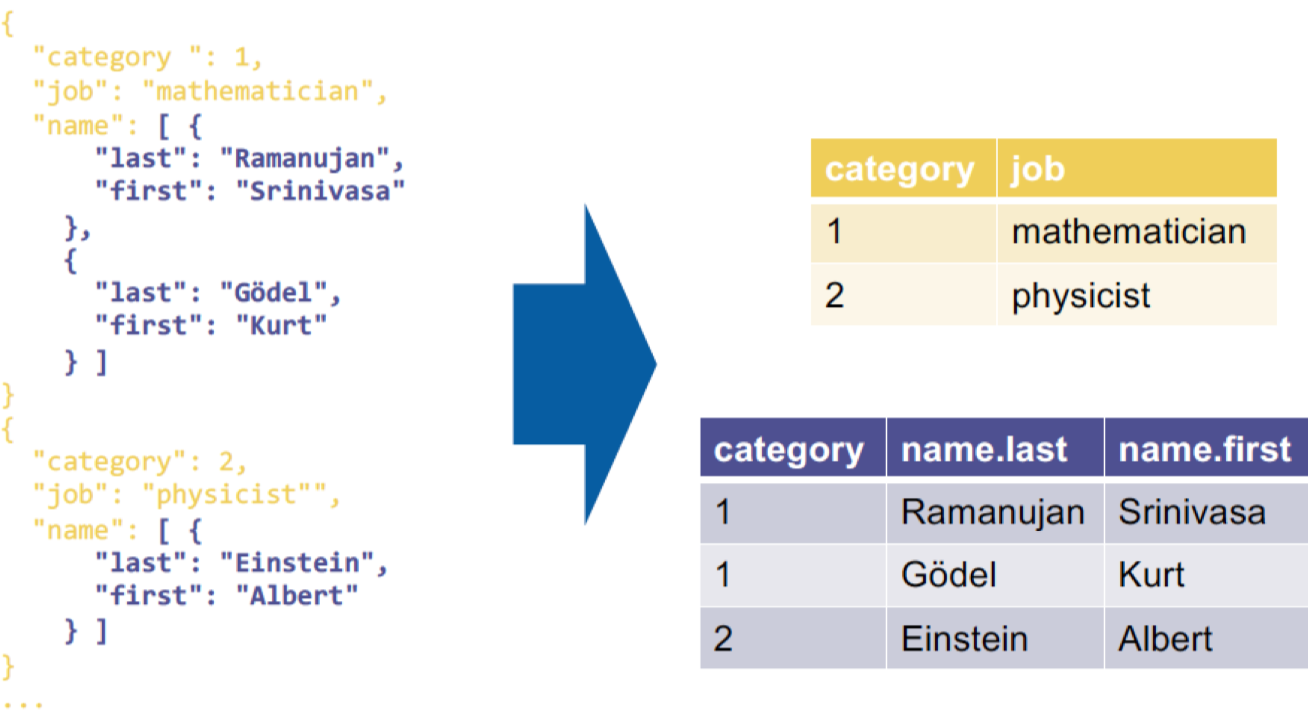
\includegraphics[width=\textwidth]{Figures/NestednessIssue.png}
        \caption{Nestedness Issue is resolved by creating two separate tables.}
    \end{subfigure}
    \hfill
    \begin{subfigure}{0.49\textwidth}
        \centering
        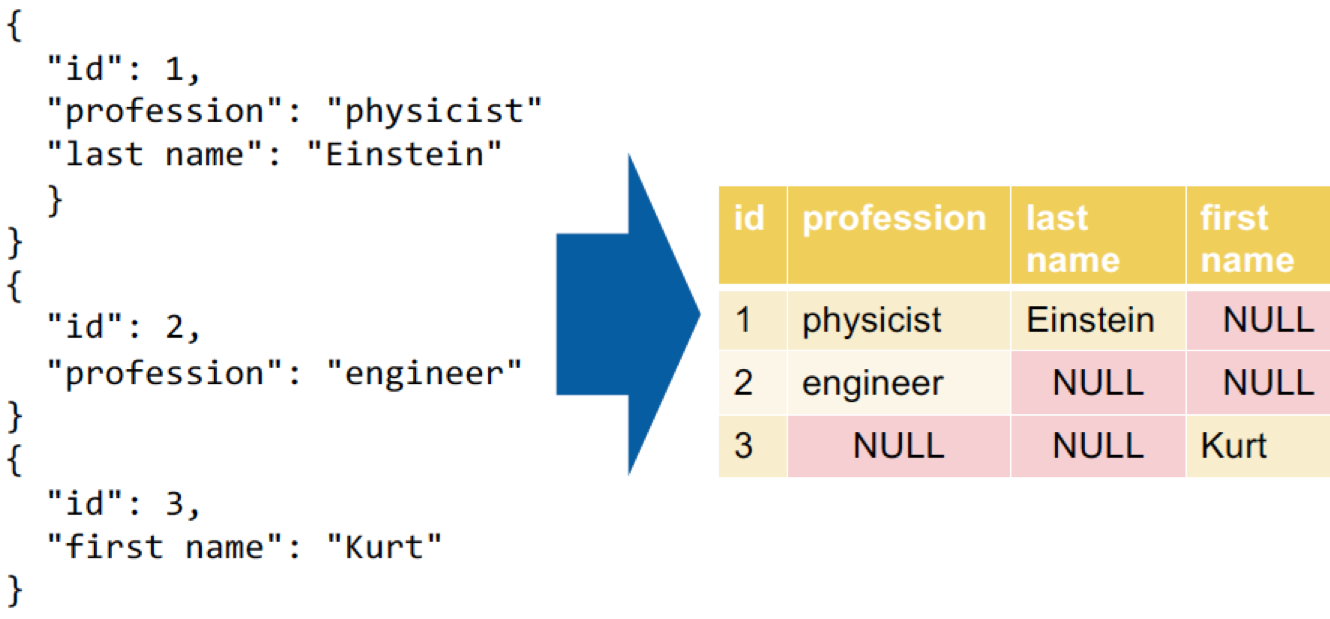
\includegraphics[width=\textwidth]{Figures/HeterogenetyIssue.png}
        \caption{Heterogeneity Issue is resolved by filling the missing values with NULL.}
    \end{subfigure}
    \caption{Nestedness and Heterogeneity Issues.}
\end{figure}

In general cases, we have a impedance mismatch. Meaning: when you have data that has a certain shape and a certain model and you try to hit it with a hammer to fit it into a different system that was designed for another shape and another model.

\subsection{Document Stores}
Document stores provide a native database management system for semi-structured data. Document stores work on collections of records, generalizing the way that relational tables can be seen as collections of rows.

Records in a document store are called documents. It is important to understand that document stores are optimized for the typical use cases of many records of small to medium sizes. Typically, a collection can have millions or billions of documents, while each single document weighs no more than 16 MB. Some document stores strictly enforce a maximum size and will not allow larger individual documents.

Finally, a collection of documents need not have a schema: it is possible to insert random documents that have dissimilar structures with no problem at all. Most document stores, however, do provide the ability to add a schema. If they do, it is then possible to validate the documents in a collection. This can be done before adding documents (schema-on-write), to ensure validity, or validation can be attempted after adding the schema to a previously schemaless collection, or while processing a collection (schema-on-read).

Document stores can generally do selection, projection, aggregation and sorting quite well, but many of them are typically not (yet) optimized for joining collections. In fact, often, their language or API does not offer any joining functionality at all, which pushes the burden to reimplement joins in a host language to the users. The same applies for complex queries that push the API to its limits and force users to write a significant part of their code in the host language, rather than push it down to the document store. This is a serious breach of data independence.


\subsubsection{Implementations}
There are many different document stores such as MongoDB, CouchDB, ElasticSearch, and many more. We will focus on MongoDB.

\subsubsection{Physical Storage}

In a data lake, the files are stored "as is" in the cloud or on a distributed file system. In a databsae management system, the storage format si typically proprietary and optimized for performance. It is hidden from the user. Just like the storage format si optimized for tabular data in a relational database management system, it is optimized for tree-like data in a cocument store.

In MongoDB, the format is a binary version fo JSON called BSON (Binary JSON). BSON is basically based on a sequence of tokens that efficiently encode the JSON constructs found in a document, like so:
\begin{align*}
    \mathrm{ \geschwungeneklammer{"foo": null} \ \Rightarrow \ 6 \ \backslash x03 \ \backslash x66 \ \backslash x6F \ \backslash x6F \ \backslash x00 \ \backslash x04 \ \backslash x00 }
\end{align*}
The immediate benefit of BSON is tha tit takes less space in storage than JSON stored as a text file. Furthermore, BSON supports additional types that JSON does not have, such as dates.

Atomicity is guaranteed on the level of documents. One can change two documents at the same time, however two users cannot access the same document at the same time.


\subsection{Querying paradigm (CRUD)}

The API of MondoDB, like many other document stores, is based on the CRUD paradigm. CRUD means Create, Read, Update, Delete and corresponds to low-level primitives.

\subsubsection{Populating a collection}
Collections in MongoDB are accessed in JavaScript via \texttt{db.scientists} where "scientists" is the name of the collection. You can insert one document with the method
\begin{lstlisting}[style=neutral]
db.scientists.insertOne(
    {
        "Last" : "Einstein",
        "Theory" : "Relativity"
    }
)
\end{lstlisting}

In order to insert several documents at the same time you can use:

\begin{lstlisting}[style=neutral]
db.scientists.insertMany(
    [
        {
            "Last" : "Lovelace",
            "Theory" : "Analytical Engine"
        },
        {
            "Last" : "Einstein",
            "Theory" : "Relativity"
        }
    ]
)
\end{lstlisting}

MongoDB automatically adds to every inserted document a special field called "\_id" and associates with a value called Object ID and with a type of its own. An Object ID can simply be thought of as a 12 byte binary value. Object Ids are convenient for deleting or updating a specific document with no ambiguity.

\subsubsection{Querying a collection}

\paragraph{Scan a collection}
Asking for the content of an entire collection is done via \texttt{db.collection.find()}. Equivalently in SQL:
\begin{lstlisting}[style=neutral]
SELECT *
FROM collection
\end{lstlisting}
This function does not in fact return the entire collection; rather, it returns some pointer, called a cursor, to the collection; the user can then iterate on the cursor in an imperative fashion in the host language (this is another reason why this is not a query language).

\paragraph{Selection}
You can perform a selection by passing one or more parameters to \texttt{find()}:
\begin{lstlisting}[style=neutral]
db.collection.find({"Theory" : "Relativity"})
db.collection.find(
    {
        "Theory" : "Relativity",
        "Last" : "Einstein"
    }
)
\end{lstlisting}
The first of the above above query returns all documents in the collection that have a key called “Theory” associated with the string value “Relativity”. The two above queries would correspond, in SQL, to a WHERE clause, like so:
\begin{lstlisting}[style=neutral]
SELECT *
FROM collection
WHERE Theory = "Relativity"

SELECT *
FROM collection
WHERE Theory = "Relativity"
  AND Last = "Einstein"
\end{lstlisting}

What is different from a relational database, then? In a document store, it is possible that some documents have this key, while others do not. The latter are excluded from the results. It is also possible that some documents have the key, but the value is something else than a string (a number, a date, etc). These documents would also be excluded from the results.

A disjunction (OR) uses a special MongoDB keyword, prefixed with a dollar sign:
\begin{lstlisting}[style=neutral]
db.collection.find(
    {
        "$or" : [
            {"Theory" : "Relativity"},
            {"Last" : "Einstein"}
        ]
    }
)
\end{lstlisting}

MongoDB offers many other keywords, for example for comparison other than equality:

\begin{lstlisting}[style=neutral]
db.collection.find(
    {
        "Publications" : { "$gte" : 100}
    }
)
\end{lstlisting}
Equivalent to:
\begin{lstlisting}[style=neutral]
SELECT *
FROM scientists
WHERE Publications >= 100
\end{lstlisting}


\paragraph{Projection}
Projections are made with the second parameter of this same find() method. This is done in form of a JSON object associating all the desired keys in the projection with the value 1.

\begin{lstlisting}[style=neutral]
db.scientists.find(
    {"Theory" : "Relativity"},
    {"First" : 1 , "Last" : 1}
)
\end{lstlisting}

Equivalently in SQL:
\begin{lstlisting}[style=neutral]
SELECT First, Last
FROM scientists
WHERE Theory = 'Relativity'
\end{lstlisting}

By default, the object ID, in the field “ id” is always included in the results. It is possible to project it away with a 0:
\begin{lstlisting}[style=neutral]
db.scientists.find(
    {"Theory" : "Relativity"},
    {"First" : 1 , "Last" : 1, "_id" : 0}
)
\end{lstlisting}
There is no SQL equivalent for this query. It is also possible to project fields away in the same way with 0s, however 1s and 0s cannot be mixed in the projection parameter, except in the specific above case of projecting away the object ID.

\paragraph{Counting} can be done via
\begin{lstlisting}[style=neutral]
db.scientists.find(
    { "Theory" : "Relativity" }
).count()
\end{lstlisting}
equivalently in SQL:
\begin{lstlisting}[style=neutral]
SELECT COUNT(*)
FROM scientists
WHERE Theory = "Relativity"
\end{lstlisting}

\paragraph{Sorting} can be done via
\begin{lstlisting}[style=neutral]
db.scientists.find(
    { "Theory" : "Relativity" },
    { "First" : 1, "Last" : 1 }
).sort({
    "First" : 1,
    "Name" : -1
})
\end{lstlisting}
equivalently in SQL:
\begin{lstlisting}[style=neutral]
SELECT First, Last
FROM scientists
WHERE Theory = "Relativity"
ORDER BY First ASC, Name DESC
\end{lstlisting}
1 stands for ascending order and -1 for descending order. You can also add for example \texttt{.skip(30).limit(10)} after the \texttt{.sort(...)} statement which is eqiuvalent to adding the following in SQL
\begin{lstlisting}[style=neutral]
LIMIT 10
OFFSET 30    
\end{lstlisting}

\paragraph{Duplicate Elimination}
You can obtain distinct values for one field with \texttt{db.scientists.distinct("Last")}.


\subsubsection{Querying for heterogeneity}

\paragraph{Absent fields}

You can also filter for the null object. It returns all objects with either the null object as the element or the objects with no entry for that argument.
\begin{lstlisting}[style=neutral]
db.scientists.find(
    {"Theory" : null}
)
\end{lstlisting}

Equivalently in SQL:
\begin{lstlisting}[style=neutral]
SELECT *
FROM scientists
WHERE Theory IS NULL
\end{lstlisting}

\paragraph{Filtering for values across types}
Querying for several values with different types and in the same field can easily be made with a disjunctive query:
\begin{lstlisting}[style=neutral]
db.collection.find(
    {
        "$or" : [
            { "Theory" : "Relativity" },
            { "Theory" : 42 },
            { "Theory" : null }
        ]
    }
) 
\end{lstlisting}

or alternatively
\begin{lstlisting}[style=neutral]
db.scientists.find(
    {
        "Theory" : {
            "$in" : [ "Relativity", 42, null ]
        }
    }
)
\end{lstlisting}


\subsubsection{Querying for Nestedness}

\paragraph{Values in nested objects}
MongoDB uses the dot syntax. This means that, like the dollar sign, dots are treated in a special way in MongoDB queries.
\begin{lstlisting}[style=neutral]
db.scientists.find({
    "Name.First" : "Albert"
})
\end{lstlisting}
The following is \underline{false}:
\begin{lstlisting}[style=neutral]
db.scientists.find({
    "Name" : {"First" : "Albert"}
})
\end{lstlisting}
This would only return the documents in which "Name" exactly matches \texttt{\{"First" : "Albert"\}}. The above query returns all the elements that \underline{contain} "Albert" as first name.

\paragraph{Values in nested arrays}
MongoDB allows to filter documents based on whether a nested array contains a specific value, like so:
\begin{lstlisting}[style=neutral]
db.scientists.find({
    "Theories" : "Special relativity"
})
\end{lstlisting}


\subsubsection{Deleting Objects from a Collection}
You can delete one or many objects from a collection by
\begin{lstlisting}[style=neutral]
db.scientists.deleteMany(
    {"century" : "15"}
)
\end{lstlisting}
or
\begin{lstlisting}[style=neutral]
db.scientists.deleteOne(
    {"century" : "15"}
)
\end{lstlisting}
The \texttt{deletaMany} command will delete \textit{all} documents matching the criteria. The \texttt{deletaOne} command will delete just one document matching the criterion, leaving any other documents matching the criterion unchanged in the original collection. If there is no such document, nothing happens.

\subsubsection{Updating Objects in a Collection}
Documents can be updated with \texttt{updateOne()} and \texttt{updateMany()} by providing both a filtering criterion (with the same syntax as the first parameter of find()) and an update to apply.
\begin{lstlisting}[style=neutral]
db.scientists.updateMany(
    {"Last" : "Einstein"},
    {$set : {"Century" : "20"}}
)
\end{lstlisting}
In addition to \$set, there are also \$unset to remove a value and \$replaceWith to completely change an entire document.
The granularity of updates is per document, that is, a single document can be updated by at most one query at the same time. However, within the same collection, several different documents can be modified concurrently by different queries in parallel.


\subsubsection{Complex Pipelines}

For grouping and such more complex queries, MongoDB provides an API in the form of aggregation pipelines:
\begin{lstlisting}[style=neutral]
db.scientists.aggregate(
    {$match : {"Century" : 20}},
    {$group : {
        "Year" : "$year$,
        "Count" : { "$sum" : 1}
        }
    }
    {$sort : {"Count" : -1}},
    {$limit : 5}
)
\end{lstlisting}
This is somewhat a "mini Spark Implementation" in MongoDB. In SQL one could write this as
\begin{lstlisting}[style=neutral]
SELECT Year, SUM(Count) AS Count
FROM scientists
WHERE Century = 20
GROUP BY Year
ORDER BY SUM(Count) DESC
LIMIT 5
\end{lstlisting}

\subsection{Architecture}

Principle: Scaling out the hardware to multiple machine, and sharding as well as replicating the data.

\subsubsection{Sharding Collections}
Collections in MongoDB can be sharded. Shards are determined by selecting one or several fields. (Lexicographically-ordered) intervals over these fields then determine the shards. This is similar in spirit to regions in HBase, which are sharded by Row ID intervals. Shards then are stored in different physical locations. The fields used to shard must be organized in a tree index structure.

\subsubsection{Replica Sets}
A replica set is a set of several nodes running the MongoDB server process. The nodes within the same replica set all have a copy of the same data. Note that this architecture is not the same as that of HDFS, in which the replicas are spread over the entire cluster with no notion of “walls” between replica sets and no two DataNodes having the exact same block replicas. It is also not the same as HBase, in which nodes receive the responsibility of handling specific regions, but do not necessarily store them physically as this is done on the HDFS level.

\begin{figure}[h]
    \centering
    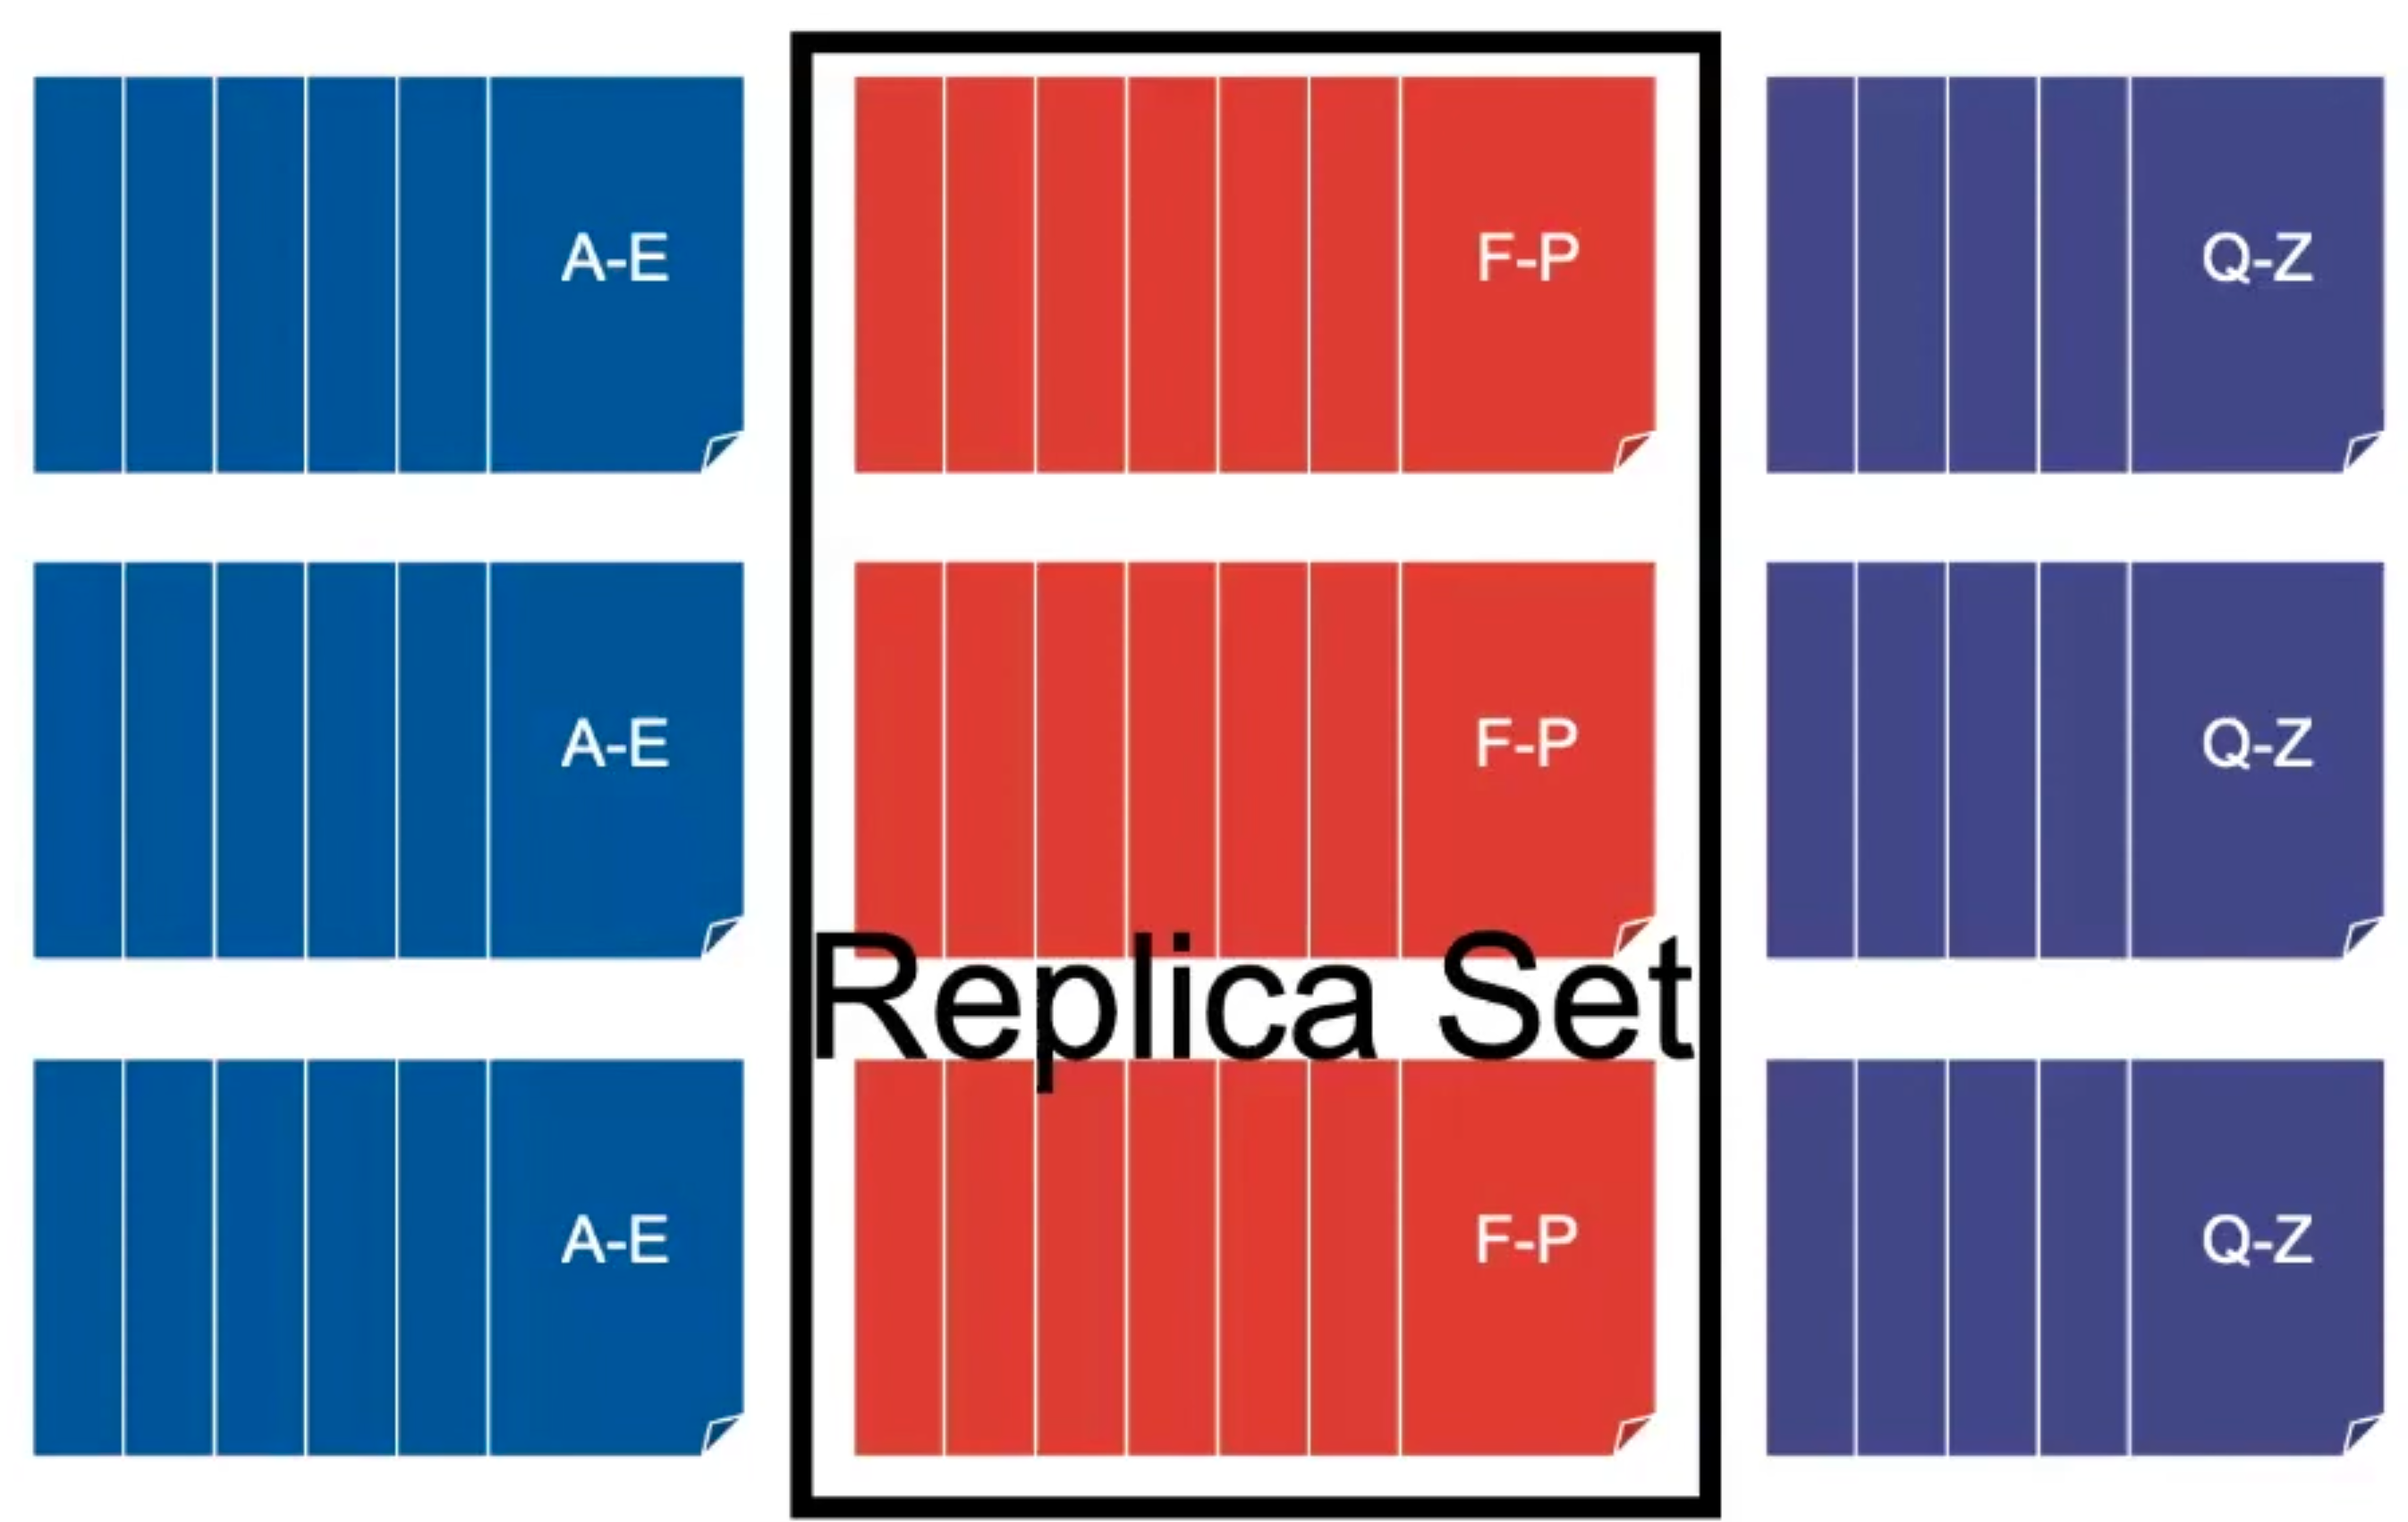
\includegraphics[width=0.5\textwidth]{Figures/DocumentStoresReplicas.png}
    \caption{Replicatoin happens vertically, and sharding horizontally.}
\end{figure}

\begin{figure}[h]
    \centering
    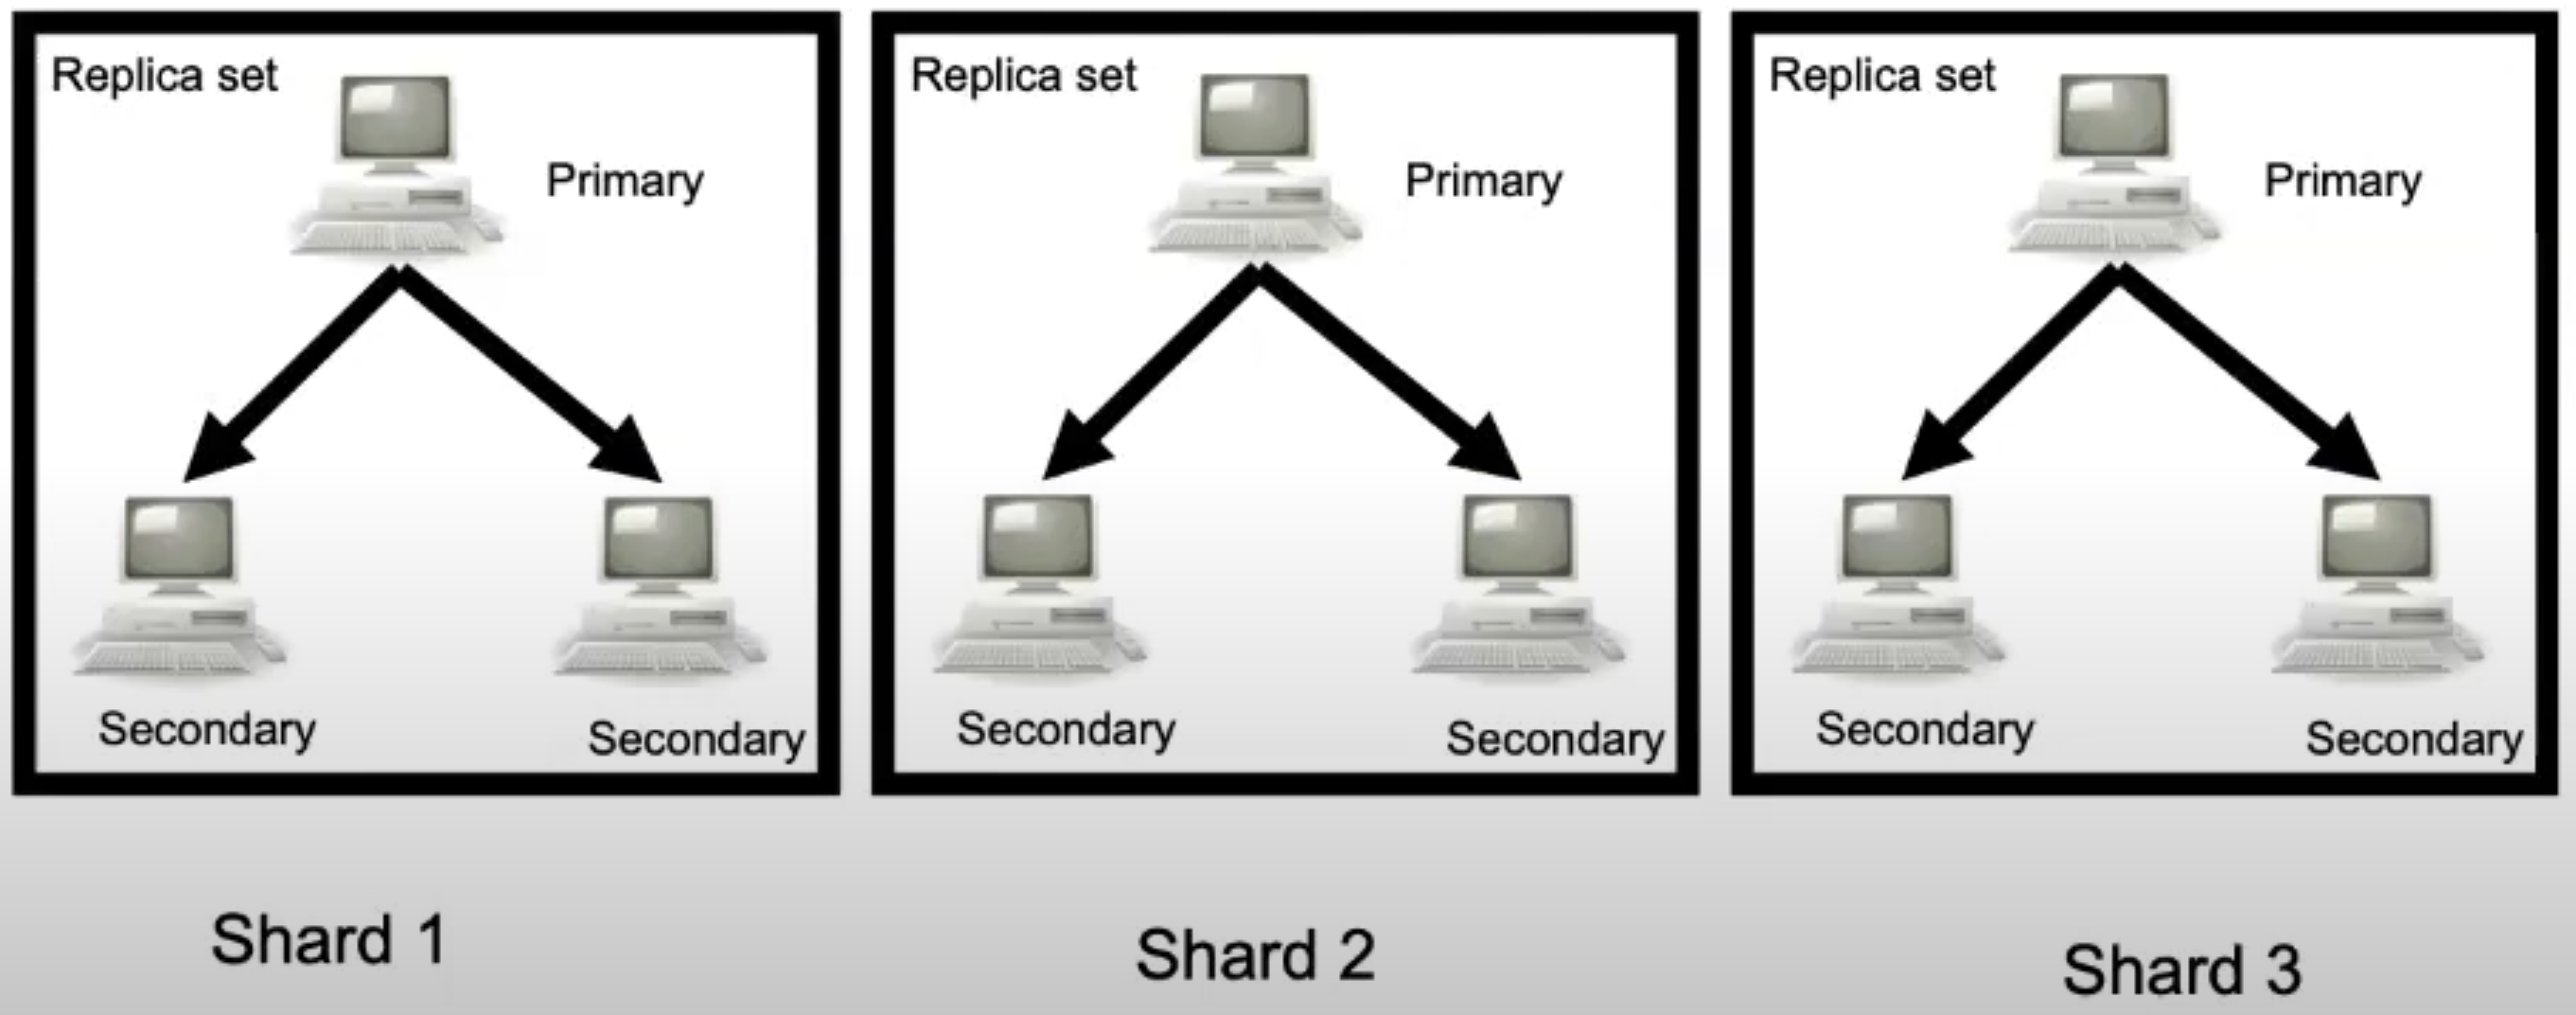
\includegraphics[width=0.8\textwidth]{Figures/DocumentStoresReplicas2.png}
    \caption{We have a coordinator node in each shard and we have worker nodes. With this we defete crashes, we don't lose data, and we can process in parallel.}
\end{figure}

\subsubsection{Write Concerns}
When writing (be it delete, update or insert) to a collection, more exactly, to a specific shard of a collection, MongoDB checks that a specific minimum number of nodes (within the replica set that is responsible for the shard) have successfully performed the update. Once the minimum number of replication is reached, the user call returns (synchronous). Then replication continues in the background to more (asynchronous).


\subsection{Indices}

\subsubsection{Motivation}
A document store, unlike a data lake, manages the physical data layout. This has a cost: the need to import (ETL) data before it is possible to query it, but this cost comes with a nice benefit: index support, just like relational database management systems.

There are different ways to look up data. Either with a point query (e.g. \texttt{find({"Name":"Euler"})}) which points to a unique document, a selection query (e.g. \texttt{find("Profession":"Mathematician")}) which points to several documents, or a range query (e.g. \texttt{find("Year":{"\$gte":1900})}).

To understand Indices, have a look at \cref{fig:Indices}. Imagine you add a structure to the list of documents, here a list of colors, sorted in a certain way, with pointers to the elements that contain that color in the document. Like this, you can lookup for example "orange" in the color list and then obtain all the pointers to the documents containing "orange" in the "Color" list. It then suffices to follow the pointer(s) to the documents with that color, which is just a disk read away.

\begin{figure}[h]
    \centering
    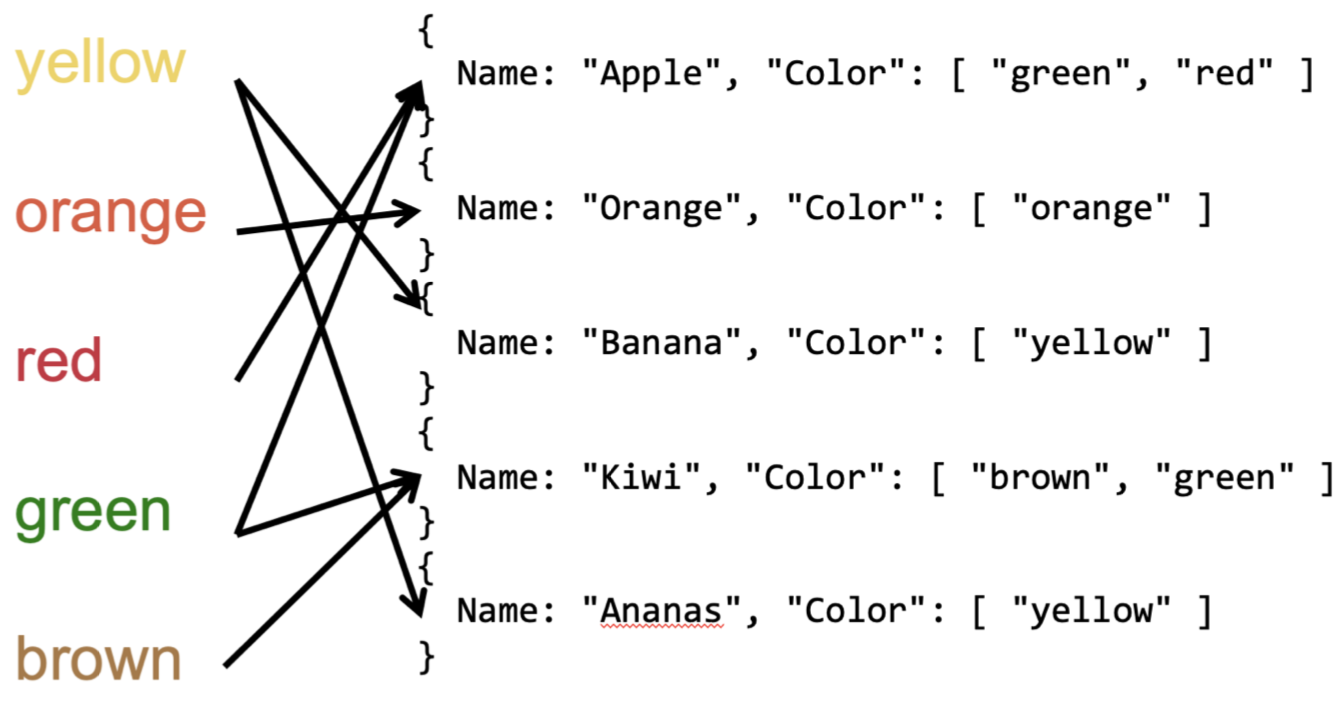
\includegraphics[width=0.7\textwidth]{Figures/Indices.png}
    \caption{Index Pointers.} \label{fig:Indices}
\end{figure}

\subsubsection{Hash Indices}

Hash indices are used to optimize point queries and more generally queries that select on a specific value of a field. The general idea is that all the values that a field takes in a specific collection can be hashed to an integer. The value, together with pointers to the corresponding documents, is then placed in a physical array in memory, at the position corresponding to this integer (modulo the
overall size of the array).

\begin{figure}[h]
    \centering
    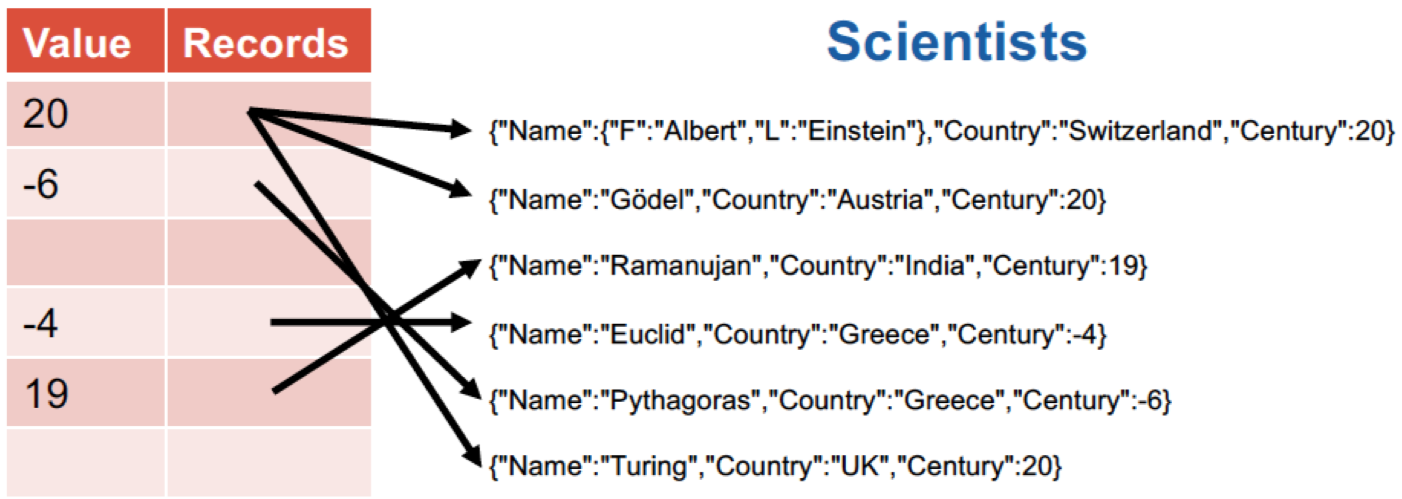
\includegraphics[width=0.6\textwidth]{Figures/HashIndexing.png}
    \caption{Hash Indices. A hash function $h$ maps the values of "Century" to an index. Here, for example $h(20)=0$, $h(-6)=1$, $h(-4) = 3$ and $h(19)=4$. Important to remember: $h$ is deterministic.}
\end{figure}

The hard part is creating the hash function $h$. Having done that, one can query extremely fast the documents in the document list. Here a code to create the hash function $h$:
\begin{lstlisting}[style=neutral]
db.scientists.createdIndex({
    "Century" : "hash"
})
\end{lstlisting}

and here a code to look up documents in the document list:
\begin{lstlisting}[style=neutral]
db.scientists.find({"Century":19})
\end{lstlisting}

Hash functions fulfill useful criteria such as making collisions unlikely, spreading values uniformly in the index array, etc. They are, in fact, more powerful than what we need, but most importantly enough powerful for what we need. Furthermore, they are very fast.

However, there is no free lunch: before an index can be used, it must be built. Building an index consists in the creation of the array structure, and then its population by sequentially scanning through the entire collection, computing the hash of the value, and adding to the index an entry and a pointer to the document, document by document.

Indices are built at the request of the user, by executing a command. Building an index can either happen synchronously, in the sense that the entire collection (or data store) remains unavailable during build time. Or it can happen asynchronously, meaning that the collection (or data store) remains available, but will be slower until the index is completely built.

\paragraph{Limitations of Hash Indices}

Hash indices to not support range queries, Hash functions are not perfect (there shouldn't be collisions, however, in real life there sometimes are collsions making it slower) and you also need a large amount of space to avoid collisions (collision means two values give the same position).

\subsubsection{Tree Indices}

Range queries are supported with tree indices. Instead of an array, tree indices use some sort of tree structure in which they arrange the possible values of the indexed field, such that the values are ordered when traversing the tree in a depth-first-search manner.

More precisely, the structure is called a B+-tree. Unlike a simple binary tree, nodes have a large number of children. The intent is that the leaves (and nodes) of the tree are large enough to match roughly a disk block, in order to optimize disk latency when fetching the nodes. In many cases, indices are so large (or numerous) that they do not fit in memory, and the database system only loads the parts of the index it needs. With nodes the size of a block, fewer disk accesses are needed.

In B+Trees it is like looking something up in a dictionary. In the example of \cref{fig:BTrees}, you look if hour is to the left or right of certain nodes. Like this, you do not need to scan the whole data. The big advantage is that you can access the data block-wise instead of bit-by-bit.

\begin{figure}[h]
    \centering
    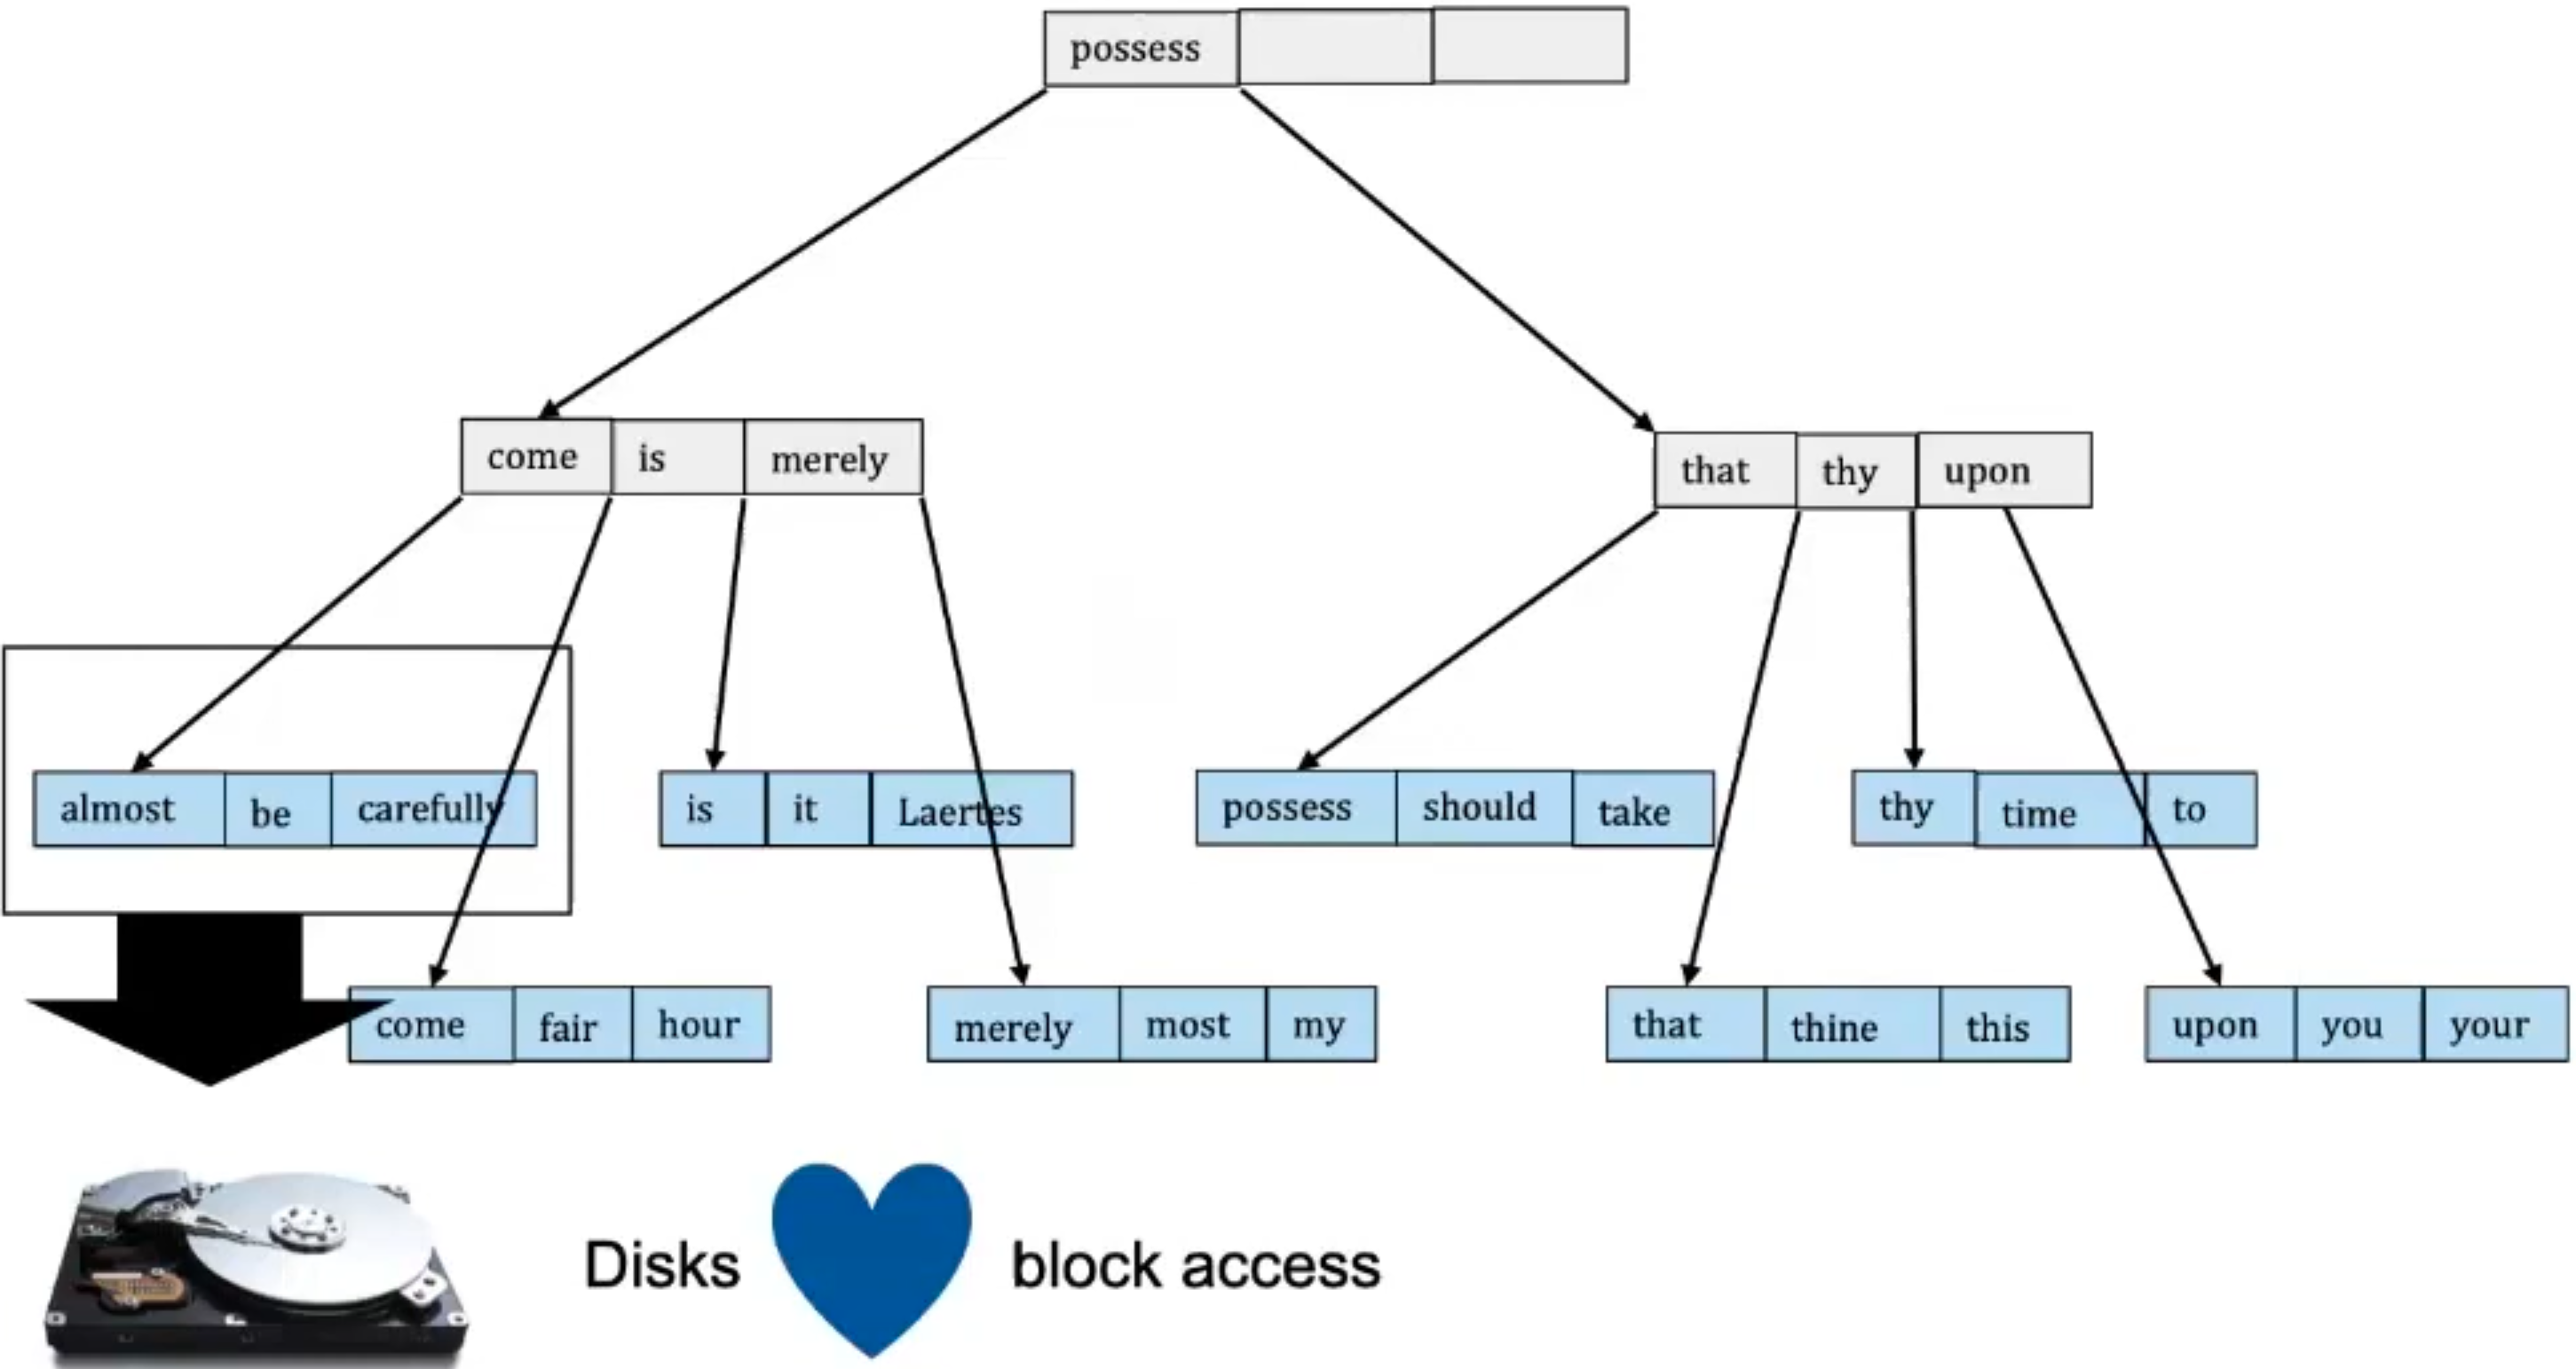
\includegraphics[width=0.7\textwidth]{Figures/B+Trees.png}
    \caption{B+Trees Illustration}\label{fig:BTrees}
\end{figure}

The code looks like this:
\begin{lstlisting}[style=neutral]
db.scientists.createIndex({
    "Century" : 1
})
\end{lstlisting}

By looking at \cref{fig:BTrees2} it is clear that range lookups are now possible. You can check for the index where for example $19$ is contained and then take all the pointers associated with the nodes to the right of the node corresponding to $19$.

\begin{figure}[h]
    \centering
    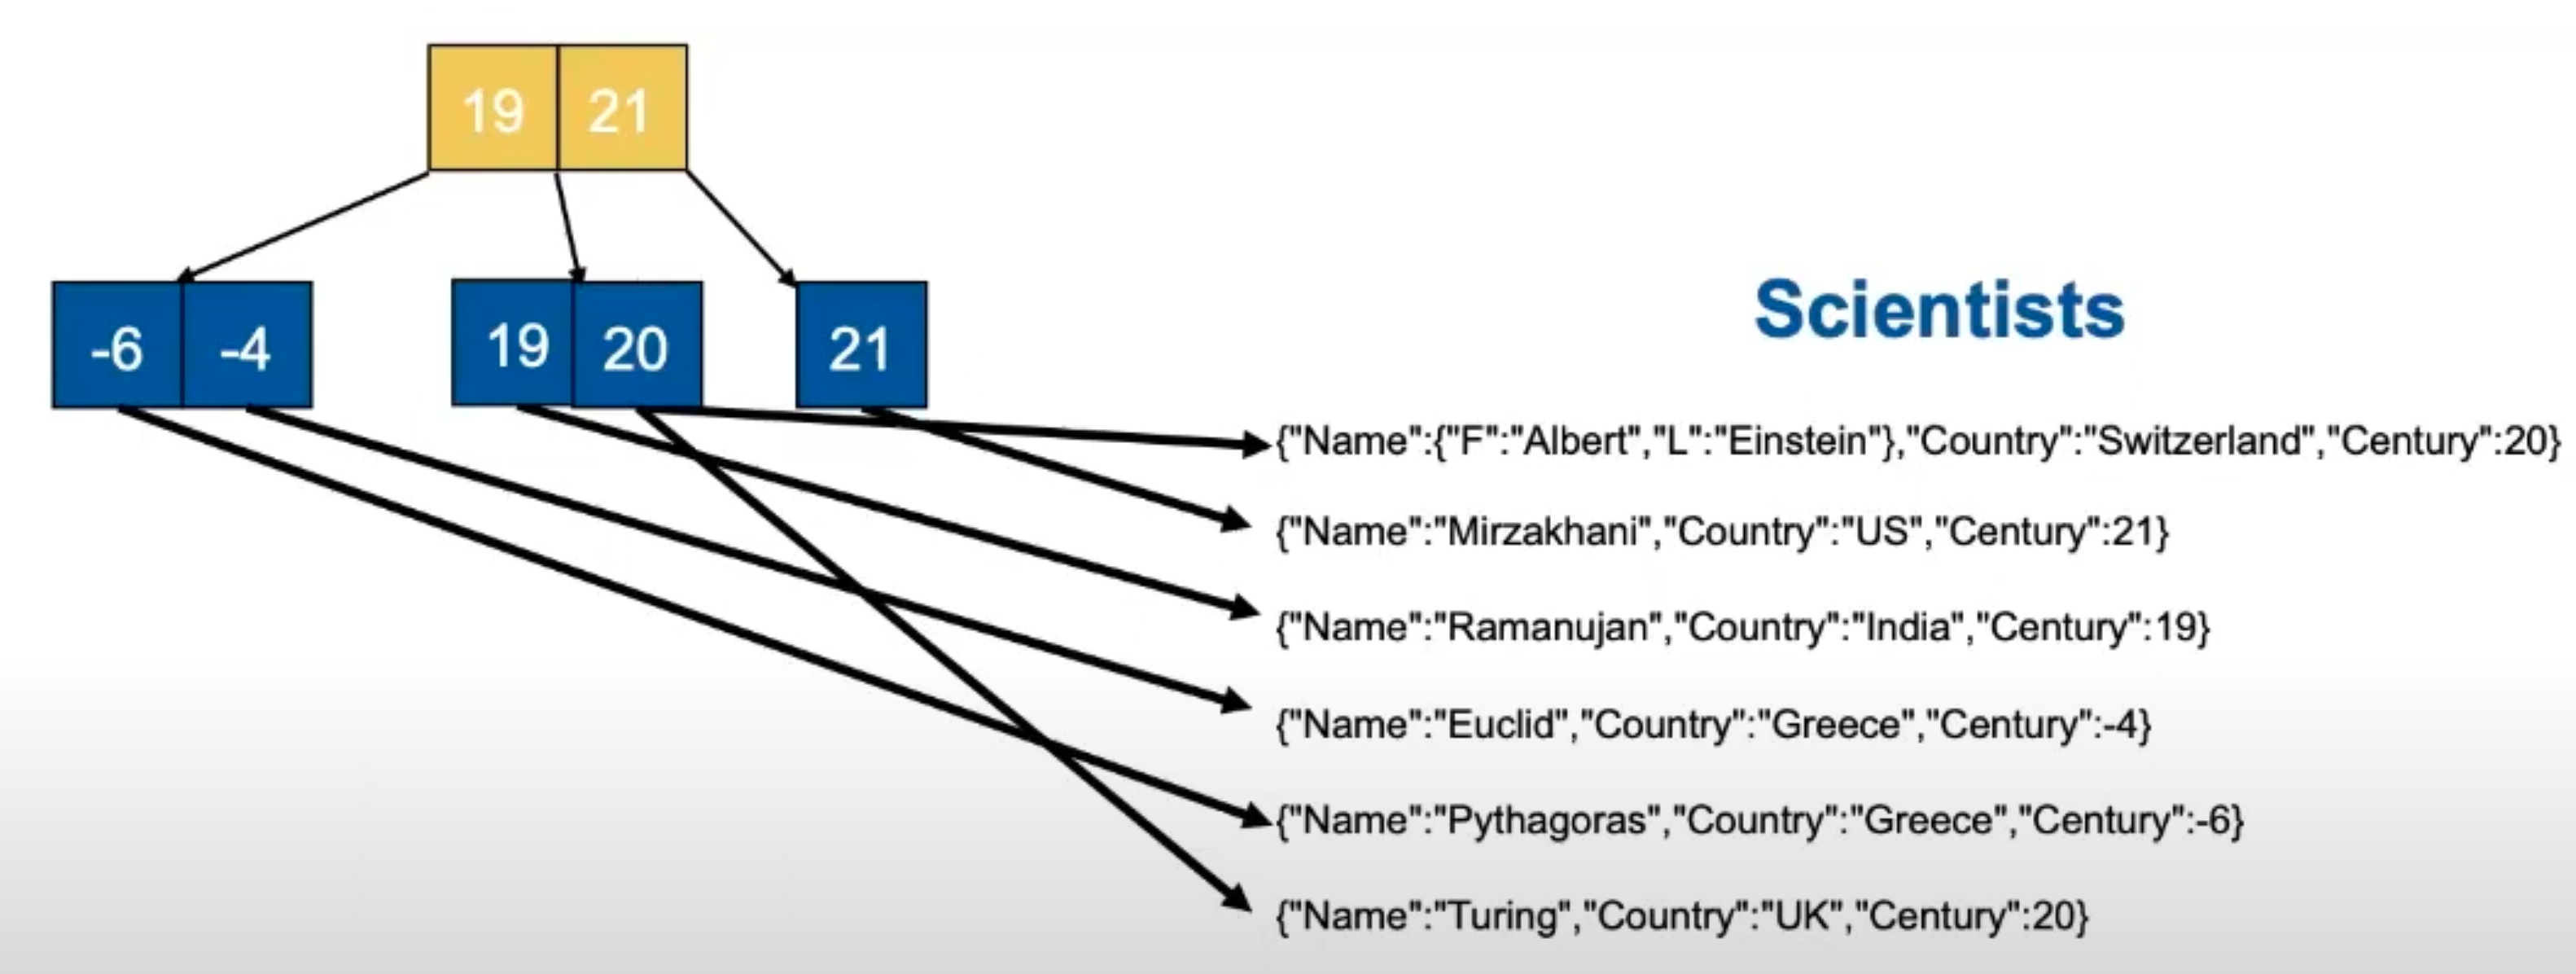
\includegraphics[width=0.7\textwidth]{Figures/BTrees.png}
    \caption{Creation of the splittings. In this example, we do not allow for blocks longer than 2. Thus, each leaf node may only have 2 elements in total. When a childnode exceeds the maximum number of elements, a new parent node is created together with another leaf containing the new datapoint. The whole tree is created in this manner. One just needs to specify how many datapoints should be in the leaf nodes. This is usually limited by memory size.}\label{fig:BTrees2}
\end{figure}

There are a few constraints in a B+-tree. First, all leaves must be at exactly the same depth. This depth grows with larger collections. Second, the number of children of each node must be within a specific interval, generally parameterized as between d + 1 and 2d + 1 with some choice of d. For pedagogical purposes, we use a small value of d on our examples, but in practice d is larger. The only exception is the root node, which is not subject to the d + 1 minimum. The root can have less children, but at least two (had it only one child, it would be useless and could be removed).

The non-leaf nodes in the tree contain a list of increasing values, interlaced with pointers to the children. These values are compared to the actually sought value in order to locate the pointer that must be followed in order to resolved this sought value. There is exactly one less value on a node than its number of children. Thus, each node has between d and 2d values.

In a B+-tree, all possible values appear on the leaves together with a pointer to the documents that contain them. The values can be “repeated” on non-leaf nodes, but values on non-leaf nodes are only used for comparison purposes. A B+-tree also typically chains all its leaves with pointers, for efficient full-traversals in ascending value order. This allows resolving a range query by only looking up the bounds in the B+-tree, and then traversing from the minimum to the maximum value.

This is unlike B-trees, in which non-leaf nodes can also contain pointers to documents.

\subsubsection{Secondary Indices}

You can create indices on secondary entries:

\begin{lstlisting}[style=neutral]
db.scientists.createIndex({
    "Name.Last" : "hash"
})
\end{lstlisting}
or
\begin{lstlisting}[style=neutral]
db.scientists.createIndex({
    "Name.Last" : 1
})
\end{lstlisting}
or when involving several fields
\begin{lstlisting}[style=neutral]
db.scientists.createIndex({
    "Name.First" : 1,
    "Name.Last" : -1
})
\end{lstlisting}

What is important to understand is that, if one builds a tree index on fields A, B, C and D, then a tree index on field A is superfluous, and so is a tree index on fields A and B, and so is a tree index on fields A, B and C. This is because looking up documents with a specific value for A only, or for A and B, or for A, B and C can be efficiently done on the index on all four fields. Why this is, is left as a very interesting exercise (hint: this is because of the lexicographic ordering).
It is a common mistake by document store users to build superfluous indices in this way, which wastes valuable space.

\subsubsection{When are indices useful}

\begin{figure}[h]
    \centering
    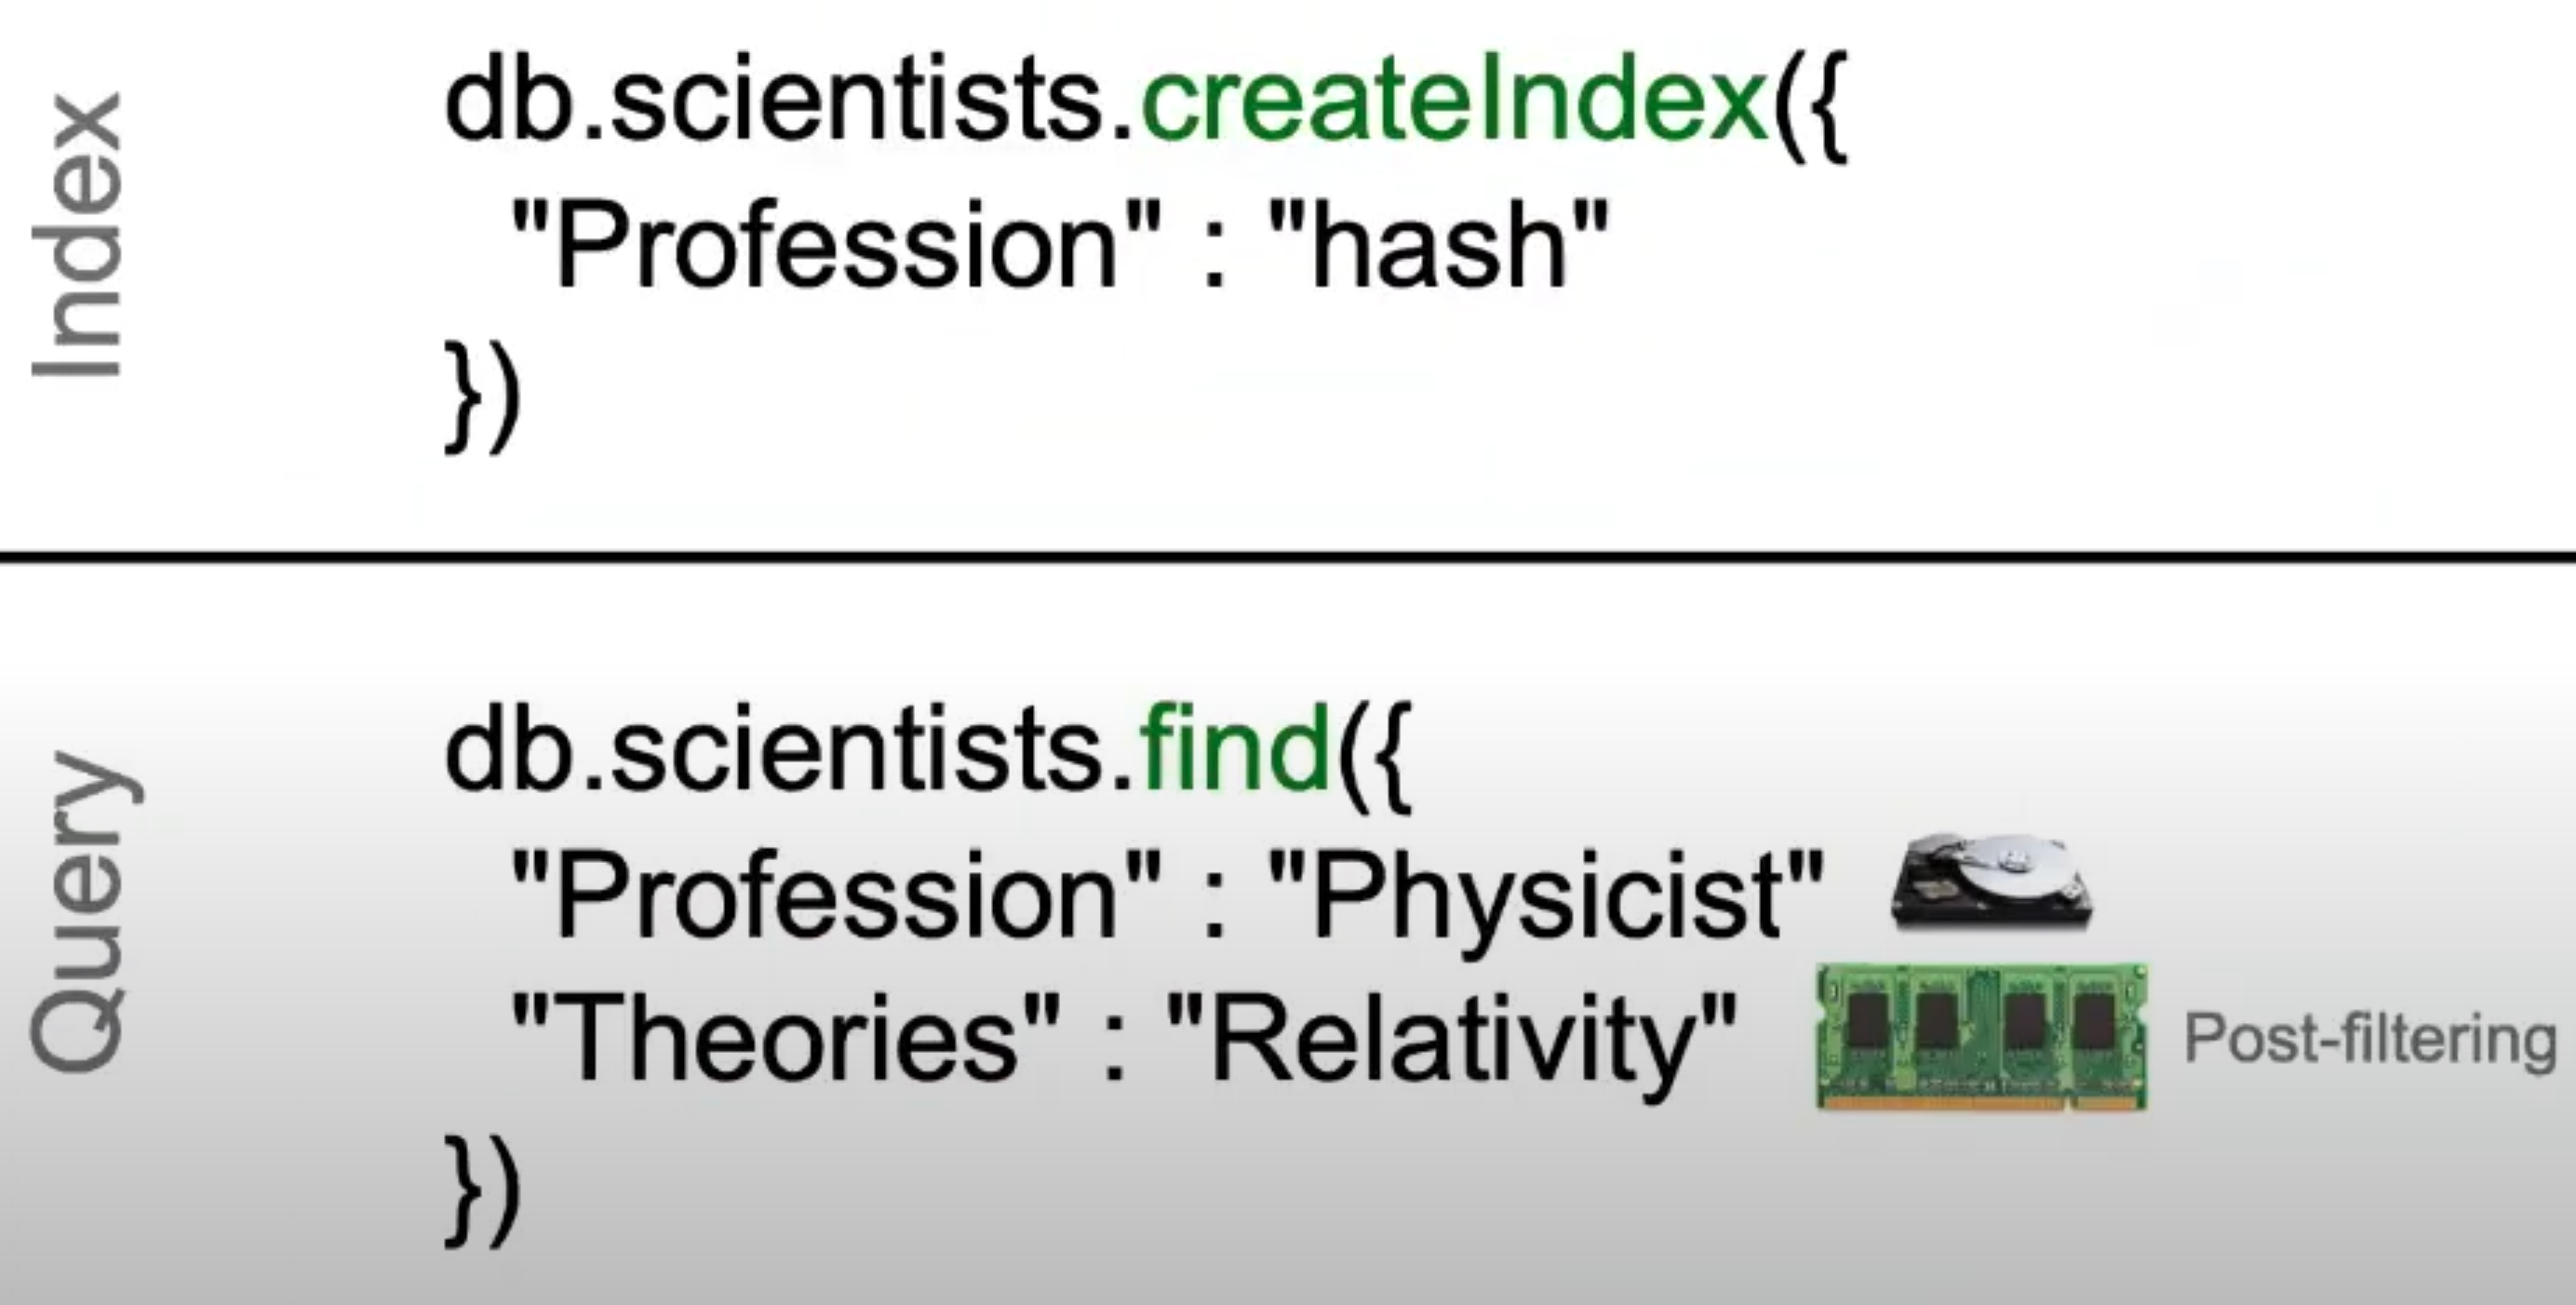
\includegraphics[width=0.5\textwidth]{Figures/IndexCreationandQuery.png}
    \caption{When creating a hash index function for one element of a document, here "Profession", then when querying the list of documents, the "Profession" is already filtered with the hash indexing, but any other filtering will be performed on the retrieved collection of documents.}
\end{figure}

You can also create and query compound indices as we have seen before:
\begin{lstlisting}[style=neutral]
db.scientists.createIndex({
    "Birth" : 1,
    "Death" : 1
})

db.scientists.find({
    "Birth" : 1887,
    "Death" : 1946
})
\end{lstlisting}

Now we can also implement range lookups:
\begin{lstlisting}[style=neutral]
db.scientists.createIndex({
    "Birth" : 1
})

db.scientists.find({
    "Birth" : {"$gte":1946}
})
\end{lstlisting}

\pagebreak

\section{Querying Denormalized Data}

\subsection{Motivation}

\subsubsection{Where are we?}

An important component which is still missing from our discussion about storage and processing of denormalized data is the query language. With what we have covered, users are left with two options to handle denormalized data:
\begin{itemize}
    \item They can use an API within an imperative host language (e.g., Pandas in Python, or the MongoDB API in JavaScript, or the Spark RDD API in Java or Scala).
    \item Or they can push SQL, including ad-hoc extensions to support nestedness, to its limits.
\end{itemize}

APIs are unsatisfactory for complex analytics use cases. They are very convenient and suitable for Data Engineers that implement more data management layers on top of these APIs, but they are not suitable for end users who want to run queries to analyse data.

There is agreement in the database community that SQL is more satisfactory for the case that data is flat and homogeneous (relational tables).

SQL, possibly extended with a few dots, lateral view syntax and explode-like functions, will work nicely for the most simple use cases. But as soon as more complex functionality is needed, this approach becomes intractable. At best, this leads to gigantic and hard-to-read SQL queries. At worst, there is no way to express the use case in SQL. In both cases, the user ends up writing most of the code in an imperative language, invoking the lower-level API or nesting and chaining simple blocks of SQL.

In this chapter we will look at a query language called JSONiq which is tailor-made for denormalized data. It offers a data-independent layer on top of both data lakes and ETL-based, database management systems, similar to what SQL offers for (flat and homogeneous) relational tables.


\subsubsection{Denormalized Data}

\begin{figure}[h]
    \centering
    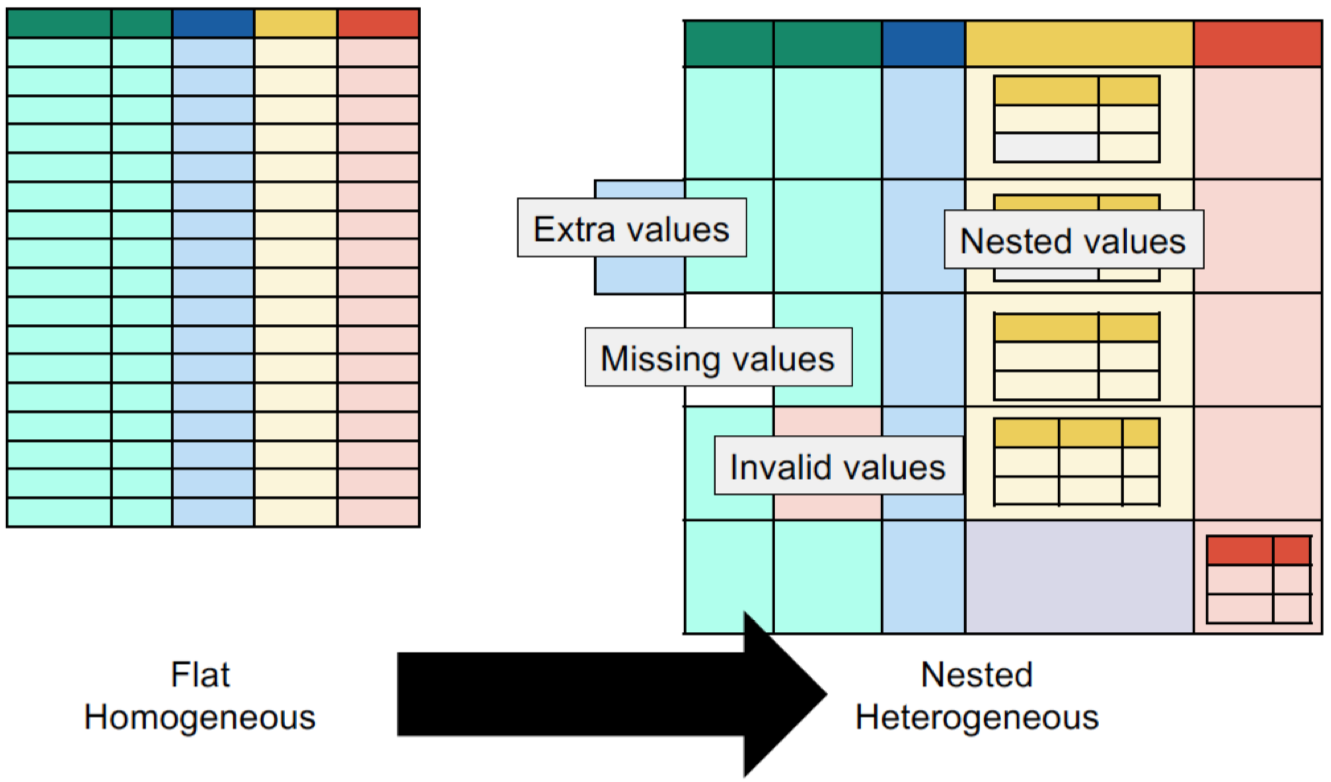
\includegraphics[width=0.7\textwidth]{Figures/DenormalizedData.png}
    \caption{Normalized vs. Denormalized Data}
\end{figure}

\subsubsection{Features of a Query Language}

A query language for datasets has three main features.

\paragraph{Declarative}
First, it is declarative. This means that the users do not focus on how the query is computed, but on what it should return. Thus, the database engine enjoys the flexibility to figure out the most efficient and fastest plan of execution to return the results.
(Python is imperative: do this, do that,... the user \underline{is} focused on how the query is computed.)

\paragraph{Functional}
Second, it is functional. This means that the query language is made of composable expressions that nest with each other, like a Lego game. Many, but not all, expressions can be seen as functions that take as input the output of their children expressions, and send their output to their parent expressions. However, the syntax of a good functional language should look nothing like a simple chain of function calls with parentheses and lambdas everywhere (this would then be an API, not a query language; examples of APIs are the Spark transformation APIs or Pandas): rather, expression syntax is carefully and naturally designed for ease of write and read. In complement to expressions, a rich function library (this time, with actual function call syntax) completes the expressions to a fully functional language.

\paragraph{Set-based}
Finally, it is set-based, in the sense that the values taken and returned by expressions are not only single values (scalars), but are large se- quences of items (in the case of SQL, an item is a row). In spite of the set-based terminology, set-based languages can still have bag or list semantics, in that they can allow for duplicates and sequences might be ordered on the logical level.


\subsubsection{JSONiq as a data calculator}

Here are some queries and their results.

\vspace{1\baselineskip}

\noindent
\begin{minipage}{0.16\textwidth}
\begin{center}
    \begin{tabular}{|c|c|}
        \hline
        Query & \texttt{1+1} \\ \hline
        Result & 2 \\ \hline
    \end{tabular}
\end{center}
\end{minipage}
\begin{minipage}{0.2\textwidth}
\begin{center}
    \begin{tabular}{|c|c|}
        \hline
        Query & \texttt{3+2*4} \\ \hline
        Result & 11 \\ \hline
    \end{tabular}
\end{center}
\end{minipage}
\begin{minipage}{0.2\textwidth}
\begin{center}
    \begin{tabular}{|c|c|}
        \hline
        Query & \texttt{2 < 5} \\ \hline
        Result & true \\ \hline
    \end{tabular}
\end{center}
\end{minipage}
\begin{minipage}{0.3\textwidth}
\begin{center}
    \begin{tabular}{|l|l|}
        \hline
        \multirow{2}{*}{Query} & \texttt{let \$i := 2} \\
         & \texttt{return \$i +1} \\ \hline
        Result & 3 \\ \hline
    \end{tabular}
\end{center}
\end{minipage}

\vspace{1\baselineskip}

\noindent
\begin{minipage}{0.2\textwidth}
\begin{center}
    \begin{tabular}{|c|c|}
        \hline
        Query & \texttt{[1,2,3]} \\ \hline
        Result & \texttt{[1,2,3]} \\ \hline
    \end{tabular}
\end{center}
\end{minipage}
\begin{minipage}{0.3\textwidth}
\begin{center}
    \begin{tabular}{|c|c|}
        \hline
        Query & \texttt{\{ "foo" : 1 \}} \\ \hline
        Result & \texttt{\{ "foo" : 1 \}} \\ \hline
    \end{tabular}
\end{center}
\end{minipage}
\begin{minipage}{0.3\textwidth}
\begin{center}
    \begin{tabular}{|c|c|}
        \hline
        Query & \texttt{\{ "foo" : 1 \}.foo} \\ \hline
        Result & \texttt{1} \\ \hline
    \end{tabular}
\end{center}
\end{minipage}

\vspace{1\baselineskip}

\noindent
\begin{minipage}{0.25\textwidth}
\begin{center}
    \begin{tabular}{|c|c|}
        \hline
        Query & \texttt{[1,2,3][[1]]} \\ \hline
        Result & \texttt{1} \\ \hline
    \end{tabular}
\end{center}
\end{minipage}
\begin{minipage}{0.5\textwidth}
\begin{center}
    \begin{tabular}{|c|c|}
        \hline
        Query & \texttt{\{ "foo" : [3,4,5] \}.foo[[1]] + 3} \\ \hline
        Result & \texttt{6} \\ \hline
    \end{tabular}
\end{center}
\end{minipage}

\vspace{1\baselineskip}

\noindent
\begin{minipage}{0.4\textwidth}
\begin{center}
    \begin{tabular}{|c|c|}
        \hline
        Query & \texttt{\{ "foo" : [3,4,5] \}.foo[]} \\ \hline
        \multirow{3}{*}{Result} & \texttt{3} \\
         & \texttt{4} \\
         & \texttt{5} \\ \hline
    \end{tabular}
\end{center}
\end{minipage}
\begin{minipage}{0.2\textwidth}
\begin{center}
    \begin{tabular}{|c|c|}
        \hline
        Query & \texttt{1 to 4} \\ \hline
        \multirow{4}{*}{Result} & \texttt{1} \\
            & \texttt{2} \\
            & \texttt{3} \\
            & \texttt{4} \\ \hline
    \end{tabular}
\end{center}
\end{minipage}
\begin{minipage}{0.4\textwidth}
\begin{center}
    \begin{tabular}{|l|l|}
        \hline
        \multirow{2}{*}{Query} & \texttt{for \$i in 3 to 5} \\
         & \texttt{return \{ \$i : \$i * \$i \} } \\ \hline
        \multirow{3}{*}{Result} & \texttt{9} \\
            & \texttt{16} \\
            & \texttt{25} \\ \hline
    \end{tabular}
\end{center}
\end{minipage}

\vspace{1\baselineskip}

\noindent
\begin{minipage}{0.66\textwidth}
\begin{center}
    \begin{tabular}{|l|l|}
        \hline
        \multirow{4}{*}{Query} & \texttt{keys(} \\
            & \texttt{  for \$i in json-file("s3://bucket/myfiles/json/*")} \\
            & \texttt{  return \$i} \\
            & \texttt{)} \\ \hline
        \multirow{2}{*}{Result} & \texttt{"foo"} \\
            & \texttt{"bar"} \\ \hline
    \end{tabular}
\end{center}
\end{minipage}

\vspace{1\baselineskip}

\noindent
\begin{minipage}{0.72\textwidth}
\begin{center}
    \begin{tabular}{|l|l|}
        \hline
        \multirow{6}{*}{Query} & \texttt{keys(} \\
            & \texttt{  for \$i in parquet-file( "s3://bucket/myfiles/parquet" )} \\
            & \texttt{  return \$i} \\
            & \texttt{)} \\ \hline
        \multirow{2}{*}{Result} & \texttt{"foo"} \\
            & \texttt{"bar"} \\ \hline
    \end{tabular}
\end{center}
\end{minipage}


\subsection{The JSONiq Data Model}

Every expression of the JSONiq "data calculator" returns a sequence of items. Always. An item can be either an object, an array, an atomic item, or a function item.
Atomic items can be any of the "core" JSON types: strings, numbers (integers, decimals, doubles...), booleans and nulls, but JSONiq has a much richer type system. You can also have Objects (\texttt{\{"foo" : "bar"\}}) and Arrays (\texttt{$[$"foo","bar"$]$}).

Sequences of items are flat, in that sequences cannot be nested. But they scale massively and can contain billions or trillions of items. The only way to nest lists is to use arrays (which can be recursively nested). Sequences can be homogeneous or heterogeneous. One item is logically the same as a sequence of one item. A sequence can also be empty. Caution, the empty sequence is not the same logically as a null item.

\begin{figure}[h]
    \centering
    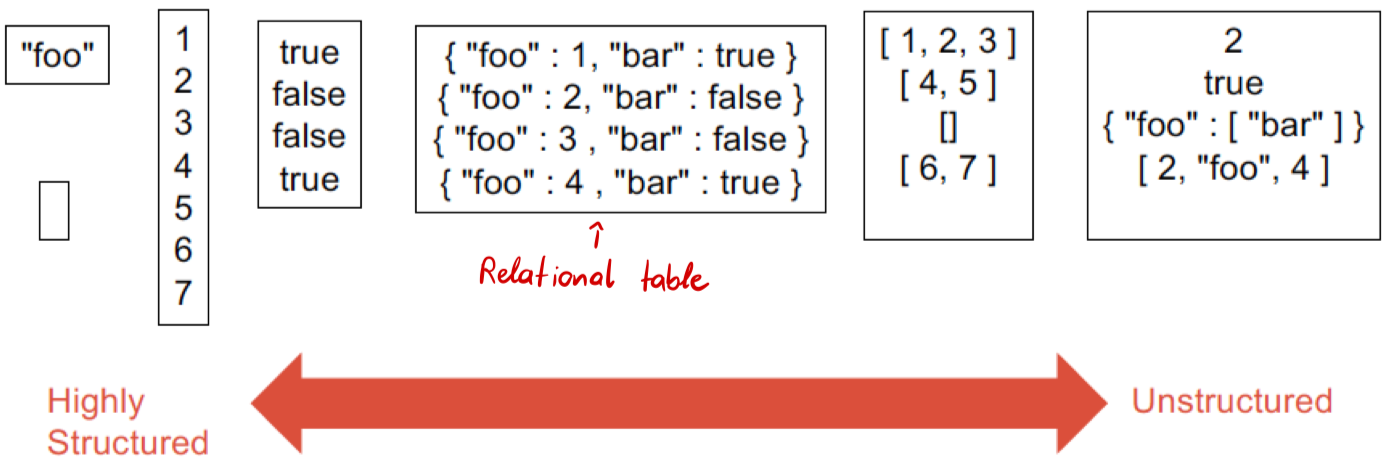
\includegraphics[width=0.7\textwidth]{Figures/SequenceofItems.png}
    \caption{Sequences of Items}
\end{figure}

\subsection{Navigation}

Assume we have a JSON document with the name file.json and the following content:
\begin{lstlisting}[style=json]
{
    "o" : [
        { "a" : {
                "b" : [
                    { "c" : 1, "d" : "a" }
                ]
            }
        },
        { "a" : {
                "b" : [
                    { "c" : 1, "d" : "f" },
                    { "c" : 2, "d" : "b" }
                ]
            }
        },
        ...,
        { "a" : {
                "b" : [
                  { "c" : 3, "d" : "l" },
                  { "c" : 1, "d" : "m" },
                  { "c" : 0, "d" : "k" }
                ]
            }
        }
    ]
}
\end{lstlisting}

\paragraph{Open File}
We can open this document and return its content with \texttt{json-doc("file.json")}. The return is the same as the whole file.

\paragraph{Object Lookups}
It is possible to navigate into objets with dots, similar to object-oriented programming. For example \texttt{json-doc("file.json").o} returns the value associated with the key \texttt{o}. This returned an array, more precisely, a sequence of one array item.

\paragraph{Array Unboxing}
We can unbox the array, meaning, extract its members as a sequence of object items, with empty square brackets, like so: \texttt{json-doc("file.json").o[]}

\paragraph{Parallel Navigation}
The dot syntax, in fact, works on sequences, too. It will extract the value associated with a key in every object of the sequence (anything else than an object is ignored and thrown away):

\begin{lstlisting}[style=json]
// Query:
json-doc("file.json").o[].a

// Result:
{ "b" : [ { "c" : 1, "d" : "a" }]}
{ "b" : [ { "c" : 1, "d" : "f" },
          { "c" : 2, "d" : "b" } ] }
{ "b" : [ { "c" : 4, "d" : "e" },
          { "c" : 8, "d" : "d" },
          { "c" : 3, "d" : "c" } ] }
{ "b" : [ ] }
{ "b" : [ { "c" : 3, "d" : "h" } ] }
{ "b" : [ { "c" : 4, "d" : "g" } ] }
{ "b" : [ { "c" : 3, "d" : "l" } ] }
\end{lstlisting}

Array unboxing works on sequences, too. Note how all the members are concatenated to a single, merged sequence, similar to a flatMap in Apache Spark.

\begin{lstlisting}[style=json]
// Query:
json-doc("file.json").o[].a.b[]

// Result:
{ "c" : 1, "d" : "a" }
{ "c" : 1, "d" : "f" }
{ "c" : 2, "d" : "b" }
{ "c" : 4, "d" : "e" }
{ "c" : 8, "d" : "d" }
{ "c" : 3, "d" : "c" }
{ "c" : 3, "d" : "h" }
{ "c" : 4, "d" : "g" }
{ "c" : 3, "d" : "l" }
\end{lstlisting}

\paragraph{Filtering with predicates}
It is possible to filter any sequence with a predicate, where \$\$ in the predicate refers to the current item being tested.

\begin{lstlisting}[style=json]
// Query:
json-doc("file.json").o[].a.b[][$$.c = 3]

// Result:
{ "c" : 3, "d" : "c" }
{ "c" : 3, "d" : "h" }
{ "c" : 3, "d" : "l" }
\end{lstlisting}

It is also possible to access the item at position n in a sequence with this same notation: if what is inside the square brackets is a Boolean, then it acts as a filtering predicate; if it is an integer, it acts as a position (we start counting at 1):

\begin{lstlisting}[style=json]
// Query:
json-doc("file.json").o[].a.b[][5]

// Result:
{ "c" : 8, "d" : "d" }
\end{lstlisting}

\paragraph{Array Lookup}
To access the n-th member of an array, you can use double-squarebrackets, like so:

\begin{lstlisting}[style=json]
// Query:
json-doc("file.json").o[[2]].a

// Result:
{"b":[{ "c" : 1, "d" : "f" },
      { "c" : 2, "d" : "b" } ] }
\end{lstlisting}

Like dot object navigation and unboxing, double square brackets (array navigation) work with sequences as well. For any array that has less elements than the requested position, as well as for items that are not arrays, no items are contributed to the output:

\begin{lstlisting}[style=json]
// Query:
json-doc("file.json").o[].a.b[[2]]

// Result:
{ "c" : 2, "d" : "b" }
{ "c" : 8, "d" : "d" }
\end{lstlisting}

\paragraph{A common pitfall: Array lookup vs. Sequence predicates}
Do not confuse sequence positions (single square brackets) with array positions (double square brackets)! The difference is easy to see on a simple example involving a sequence of two arrays with two members each:

\begin{lstlisting}[style=json]
// Query:
([1,2],[3,4])[2]
// Result:
[3,4]

// Query:
([1,2],[3,4])[[2]]
// Result:
2
4
\end{lstlisting}


\subsection{Schema Discovery}

\paragraph{Collections}
Many datasets are in fact found in the form of large collections of smaller objects. Such collections are accessed with a function call together with a name or (if reading from a data lake) a path. The name of the function can vary and in this Chapter we will just use the W3C-standard collection function. In RumbleDB, a JSON Lines dataset is accessed with the function json-line, in a similar way.

\begin{lstlisting}[style=json]
// Query:
collection( "https://www.rumbledb.org/samples/git-archive.jsonl" )

// Result:
{ "id" : "7045118886", "type" : "PushEvent", ...
{ "id" : "7045118891", "type" : "PushEvent", ...
{ "id" : "7045118892", "type" : "PullRequestEvent", ...
...
\end{lstlisting}

You can also at the first element of the collection or at the top N objects using the position function in a predicate, which returns the position in the sequence of the current item being tested by the predicate (similar to the LIMIT clause in SQL):

\begin{lstlisting}[style=json]
// Query:
collection( "https://www.rumbledb.org/samples/git-archive.jsonl" )[1]

// Result:
{ "id" : "7045118886", "type" : "PushEvent", ...

// Query:
collection( "https://www.rumbledb.org/samples/git-archive.jsonl" )[position() le 3]

// Result:
{ "id" : "7045118886", "type" : "PushEvent", ...
{ "id" : "7045118891", "type" : "PushEvent", ...
{ "id" : "7045118892", "type" : "PullRequestEvent", ...
\end{lstlisting}

\paragraph{Getting all top-level keys}
The keys function retrieves all keys. It can be called on the entire sequence of objects and will return all unique keys found (at the top level) in that collection:

\begin{lstlisting}[style=json]
// Query:
keys(collection( "https://www.rumbledb.org/samples/git-archive.jsonl" ))

// Result:
"repo"
"org"
"actor"
"public"
"type"
"created_at"
"id"
"payload"
\end{lstlisting}

\paragraph{Getting unique values associated with a key}
With dot object lookup, we can look at all the values associated with a key like so:

\begin{lstlisting}[style=json]
// Query:
collection( "https://www.rumbledb.org/samples/git-archive.jsonl" ).type

// Result:
"PushEvent"
"PushEvent"
"PullRequestEvent"
"PushEvent"
...
\end{lstlisting}

With distinct-values, it is then possible to eliminate duplicates and look at unique values:

\begin{lstlisting}[style=json]
// Query
distinct-values(collection( "https://www.rumbledb.org/samples/git-archive.jsonl" ).type)

// Result:
"PullRequestEvent"
"MemberEvent"
"PushEvent"
"IssuesEvent"
"PublicEvent"
...
\end{lstlisting}

\paragraph{Aggregations}
Aggregations can be made on entire sequences with a single function call. The five basic functions are count, sum, avg, min, max. Obvi- ously, the last four require numeric values and will otherwise throw an error.

\begin{lstlisting}[style=json]
// Query:
count(distinct-values(collection( "https://www.rumbledb.org/samples/git-archive.jsonl" ).type))

// Result:
3597

// Query:
count(collection( "https://www.rumbledb.org/samples/git-archive.jsonl" ))

// Result:
36577
\end{lstlisting}


\subsection{Construction}

\paragraph{Construction of atomic values}

Since it is a declarative language, you can just write them down. Atomic values that are core to JSON can be constructed with exactly the same syntax as JSON. E.g.

\begin{lstlisting}[style=json]
// Query:
"foo"

// Result:
"foo"
\end{lstlisting}

For more specific types, a cast is needed. This works with any of the atomic types. There are two syntaxes for this:

\begin{lstlisting}[style=json]
// Query:
NonNegativeInteger("42")
// or:
"42" cast as NonNegativeInteger

// Result:
42

// Other examples:
date("2013-05-01Z")
dateTimeStamp("2013-06-21-T05:00:00Z")
hexBinary("0CD7")
...
\end{lstlisting}

\paragraph{Construction of objects and arrays}
Objects and arrays are constructed with the same syntax as JSON. In fact, one can copy-paste any JSON value, and it will always be recognized as a valid JSONiq query returning that value.

\paragraph{Construction of sequences}
Sequences can be constructed (and concatenated) using commas:

\begin{lstlisting}[style=json]
// Query:
[2,3],true,"foo",{"f":1}

// Result:
[2,3]
true
"foo"
{"f":1}
\end{lstlisting}

Increasing sequences of integers can also be built with the to key-word: \texttt{1 to 100}.


\subsection{Scalar Expressions}
JSONiq supports basic arithmetic: addition (+), subtraction (-), multiplication (*), division (not a slash, but \texttt{div}), integer division (idiv) and modulo (mod). If both sides have exactly one item, the semantics is relatively natural.

If one side is a double and the other is a float or a decimal, a double is returned. If one side is a float and the other is a decimal, then a float is returned. If one side is a decimal and the other an integer, a decimal is returned.

If one side (or both) is the empty sequence, then the arithmetic expression returns an empty sequence without an error. If one of the two sides is null (and the other side is not the empty sequence), then the arithmetic expression returns null. If one of the sides (or both) is not a number, null, or the empty sequence, then a type error is thrown (for example when one side is a string). However, if the left side is a date and the right is a duration, you cann add the two to obtain a new date.

\paragraph{String Manipulation}
You can concatenate strings in different ways:
\begin{lstlisting}[style=json]
// Queries:
"foo" || "bar"
concat("foo","bar")
// Result:
"foobar"

// Query:
string-join(("foo","bar","foobar"),"-")
// Result:
"foo-bar-foobar"

// Query:
substr("foobar",4,3)
// Result:
"bar"

// Query:
string-length("foobar")
// Result:
6
\end{lstlisting}

\paragraph{Value Comparison}
Sequences of one atomic item can be compared.
\begin{lstlisting}[style=json]
// Queries:
1+1 eq 2
1+1 = 2
// Result
true

// Query:
6*7 ne 21*2
6*7 != 21*2
// Result:
false

// Query:
234 gt 123
// Result:
true

// Query:
null le 2
// Result:
null
\end{lstlisting}

If one of the two sides is the empty sequence, then the value com- parison expression returns an empty sequence as well.

You cannot compare strings with integers, that will through an error (but MongoDB won't).


\paragraph{General Comparison}
Comparison also works on sequences. When you try to apply a comparison to a sequence, it tries to find a match on both sides. It will return true if it finds an item in the sequence on the left matching the value on the right, that fulfil the criteria. It basically applies an existential quantification ("it exists" on the left and on the right.)
\begin{lstlisting}[style=json]
// Query:
(1,2,3,4,5) = 1
// Result:
true

// Query:
(1,2,3,4,5) < (2,3,4,5,6)
// Result
true

// Query
(1,2,3,4,5) >= (6,7,8,9,10)
// Result
false
\end{lstlisting}
The second example is true because it compares it elementwise. So because $1$ is smaller then for example $3$, it will already return true. In the third example there is no element in the left sequence larger than any of the elements in the right sequence, thus it will return false.

You will get an error if one of the elements in the sequence is a string. Furthermore, you will always get \texttt{false} if you apply a comparison ot an empty sequence. Think about it as "the empty sequence is, well, empty, and thus there cannot exist any element matching (or greater than or ...) any of the elements in the other sequence on the other side of the comparison".

\paragraph{Logic}
JSONiq supports the three basic logic expressions and, or, and not. not has the highest precedence, then and, then or.

\begin{lstlisting}[style=json]
// Query:
1+1 eq 2 and (2+2 eq 4 or not 100 mod 5 eq 0)
// Result:
true

// Query:
every $i in 1 to 10
satisfies $i gt 0
// Result:
true

// Query:
some $i in 1 to 10
satisfies $i gt 5
// Result:
true
\end{lstlisting}


\subsection{Composablility}
JSONiq, as a functional language, is modular. This means that expressions can be combined at will, exactly like one would combine addition, multiplication, etc, at will. At least as long as the types of the ouputs and inputs are compatible.

You can also have functions inside json objects:
\begin{lstlisting}[style=json]
// Query:
{
    "attr" : string-length("foobar")
    "values" : [
        for $i in 1 to 10
        return long($i)
    ]
}
// Result:
{
    "attr" : 6
    "values" : [ 1, 2, 3, 4, 5, 6, 7, 8, 9, 10 ]
}
\end{lstlisting}

Precedence (low first):
\begin{itemize}
    \item Comma
    \item Data Flow (FLWOR, if-then-else, switch...)
    \item Logic
    \item Comparison
    \item String concatenation
    \item Range
    \item Arithmetic
    \item Path expression
    \item Filter predicates, dynamic function calls
    \item Literals, constructors and variables
    \item Function calls, named function references, inline functions
\end{itemize}

Precedence can be easily overridden with parentheses. This is often useful when one does not know the precedence ordering by heart.


\subsubsection{Data Flow}

\paragraph{if-then-else}
In an if-then-else statement, you have a condition and the actions for if the statement is true or false.

\begin{lstlisting}[style=json]
// Query:
if(count(json-file("file.json").o) gt 1000)
then "Large file!"
else "Small file."
// Result:
"Small file."
\end{lstlisting}

\paragraph{Switch}
The expression inside the swich is evaluated and an error is thrown if more than one item is returned. Then, the resulting item is compared for equality with each one of the candidate values. The result of the expression corresponding to the first match is taken, and if there are no matches, the result of the default expression is taken.

\begin{lstlisting}[style=json]
// Query:
switch(json-file("file.json").o[[1]].a.b[[1]].c)
case 1 return "one"
case 2 return "two"
default return "other"
// Result:
"one"
\end{lstlisting}

\paragraph{Try-Catch}
If the expression in the try clause is successfully evaluated, then its results are taken. If there is an error, then the results of the expression in the first catch clause matching the error is taken (* being the joker).

\begin{lstlisting}[style=json]
// Query:
try {
    date(json-file("file.json").o[[1]].a.b[[1]].c)
} catch * {
    "This is not a date!"
}
// Result:
"This is not a date!"
\end{lstlisting}


\subsection{Binding Variables with Cascades of let Clauses}
The following two queries are equivalent:

\begin{lstlisting}[style=json]
// Query 1:
json-doc("file.json").o[].a.b[].c = 1
// Query 2:
let $a := json-doc("file.json")
let $b := $a.o
let $c := $b[]
let $d := $c.a
let $e : $d.b
let $f := $d[]
let $g := $f.c
return $g = 1
// Result:
true
\end{lstlisting}

Variables in JSONiq start with a dollar sign. This way of subsequently binding variables to compute intermediate results is typical of functional language.
It is important to understand that this is not a variable assignment that would change the value of a variable. This is only a declarative binding.

\subsection{FLWOR Expressions}

One of the most important and powerful features of JSONiq is the FLWOR (for, let, where, order-by, return) expression. It corresponds to SELECT-FROM-WHERE queries in SQL, however, it is considerably more expressive and generic than them in several aspects:
\begin{itemize}
    \item In SQL, the clauses must appear in a specific order (SELECT, FROM, WHERE, GROUB BY, HAVING, ORDER BY, OFFSET, LIMIT) whereas in JSONiq, clauses can appear in any order except for the first and the last one.
    \item JSONiq supports a let clause, which does not exist in SQL. Let clauses make it very convenient to write and organize more com- plex queries.
    \item In SQL, when iterating over multiple tables in the FROM clause, they “do not see each other”, i.e., the semantics is (logically) that of a Cartesian product. In JSONiq, for clauses (which correspond to FROM clauses in SQL), do see each other, meaning that it is possible to iterate in higher and higher levels of nesting by referring to a previous for variable. This is both easier to write and read than lateral views, and it is also more expressive.
    \item The semantics of FLWOR clauses is simple, clean, and inherently functional; it is based on tuple streams containing variable bindings, which flow from clause to clause. There is no “spooky action at a distance” such as the explode() function, which indirectly causes a duplication of rows in Spark SQL.
\end{itemize}

\subsubsection{Simple Dataset}
We will work with the following datasets:

\begin{lstlisting}[style=json]
// products.json
{"pid":1, "type" : "tv", "store":1}
{"pid":2, "type" : "tv", "store":2}
{"pid":3, "type" : "phone", "store":2}
{"pid":4, "type" : "tv", "store":3}
{"pid":5, "type" : "teapot", "store":2}
{"pid":6, "type" : "tv", "store":1}
{"pid":7, "type" : "teapot", "store":2}
{"pid":8, "type" : "phone", "store":4}

// stores.json
{ "sid" : 1, "country" : "Switzerland" }
{ "sid" : 2, "country" : "Germany" }
{ "sid" : 3, "country" : "United States" }
\end{lstlisting}

\subsubsection{For Clauses}
A few examples:
\begin{lstlisting}[style=json]
// Query:
for $x in 1 to 3
return { "number": $x, "square": $x * $x }
// Result
{ "number" : 1, "square" : 1 }
{ "number" : 2, "square" : 4 }
{ "number" : 3, "square" : 9 }

// Query
for $product in json-file("products.json")
return project($product, ("type", "store"))
// Result
{"type" : "tv", "store":1}
{"type" : "tv", "store":2}
{"type" : "phone", "store":2}
...

// Query
for $product in json-file("products.json")
for $store in json-file("stores.json")[$$.sid eq $product.store]
return { "product" : $product.type, "country" : $store.country }
// Result
{"product" : "tv", "country":"Switzerland"}
{"product" : "tv", "country":"Germany"}
{"product" : "phone", "country":"Germany"}
...
\end{lstlisting}

\subsubsection{Let Clauses}
A few examples:
\begin{lstlisting}[style=json]
// Query:
for $x in 1 to 10
let $square-and-cube := ($x * $x, $x * $x * $x)
return{
    "number": $x,
    "square": $square-and-cube[1],
    "cube": $square-and-cube[2]
}
// Result:
{ "number" : 1, "square" : 1, "cube" : 1 }
{ "number" : 2, "square" : 4, "cube" : 8 }
{ "number" : 3, "square" : 9, "cube" : 27 }
{ "number" : 4, "square" : 16, "cube" : 64 }
{ "number" : 5, "square" : 25, "cube" : 125 }
{ "number" : 6, "square" : 36, "cube" : 216 }
{ "number" : 7, "square" : 49, "cube" : 343 }
{ "number" : 8, "square" : 64, "cube" : 512 }
{ "number" : 9, "square" : 81, "cube" : 729 }
{ "number" : 10, "square" : 100, "cube" : 1000 }

// Query:
for $store in json-file("stores.json")
let $product := json-file("products.json")[$store.sid eq $$.store]
return {
  "store" : $store.country,
  "available products" : [
    distinct-values($product.type)
  ]
}
// Result:
{
 "store" : "Germany",
 "available products" : [
    "tv",
    "teapot",
    "phone" ]
}
{
 "store" : "Switzerland",
 "available products" : [ "tv" ]
}
{
 "store" : "United States",
 "available products" : [ "tv" ]
}
\end{lstlisting}


\subsubsection{Where Clauses}
Where clauses are used to filter variable bindings (tuples) based on a predicate on these variables. They are the equivalent to a WHERE clause in SQL. A where clause can appear anywhere in a FLWOR expression, except that it cannot be the first clause (always for or let) or the last clause (always return).

A where clause always outputs a subset (or all) of its incoming tuples, without any alteration. In the case that the predicate always evaluates to true, it forwards all tuples, as if there had been no where clause at all. In the case that the predicate always evaluates to false, it outputs no tuple and the FLWOR expression will then return the empty sequence, with no need to further evaluate any of the remaining clauses.

An example:

\begin{lstlisting}[style=json]
// Query
for $product in json-file("products.json")
let $store := json-file("stores.json")[$$.sid eq $product.store]
where $store.country = "Germany"
return $product.type
// Result
"tv"
"phone"
"teapot"
"teapot"
\end{lstlisting}

\subsubsection{Order by Clauses}
Order by clauses are used to reorganize the order of the tuples, but without altering them. In case of ties between tuples, the order is arbitrary. But it is possible to sort on another variable in case there is a tie with the first one (compound sorting keys).
A few examples:

\begin{lstlisting}[style=json]
// Query:
for $x in -2 to 2
let $square := $x * $x
order by $square descending, $x ascending
return {
  "number": $x,
  "square": $square
}
// Result:
{ "number" : -2, "square" : 4 }
{ "number" : 2, "square" : 4 }
{ "number" : -1, "square" : 1 }
{ "number" : 1, "square" : 1 }
{ "number" : 0, "square" : 0 }

// Query:
for $product in json-file("products.json")
let $store := json-file("stores.json")[$$.sid eq $product.store]
group by $t := $product.type
order by count($store) descending, string-length($t) ascending
return $t
// Result:
"tv"
"teapot"
"phone"
\end{lstlisting}

\subsubsection{Groub by Clauses}
Group by clauses organize tuples in groups based on matching keys, and then output only one tuple for each group, aggregating other variables.
However, JSONiq's group by clauses are more powerful and expres- sive than SQL GROUP BY clauses: indeed, it is also possible to opt out of aggregating other (non-grouping-key) variables. Then, for a non-aggregated variable, the sequence of all its values within a group will be rebound to this same variable as a single binding in the outcoming tuple. It is thus possible to write many more queries than SQL would allow, which is one of the reasons why a language like JSONiq should be preferred for nested datasets.
A few examples:

\begin{lstlisting}[style=json]
// Query:
for $x in 1 to 5
let $y := $x mod 2
group by $y
return {
    "grouping key" : $y,
    "grouped x values" : [ $x ],
}
// Result:
{
    "grouping key" : 0,
    "grouped x values" : [ 2, 4 ]
}
{
    "grouping key" : 1,
    "grouped x values" : [ 1, 3, 5 ]
}

// Query:
for $product in json-file("products.json")
group by $sid := $product.sid
order by $sid
let $store := json-file("stores.json")
                [$$.sid = $sid]
return {|
  $store,
  { "products" : [ distinct-values($product.type) ] }
|}
// Result:
{
    "sid" : 1,
    "country" : "Switzerland",
    "products"  [ "tv" ]
}
{
    "sid" : 2,
    "country" : "Germany",
    "products" : [ "tv", "phone", "teapot" ]
}
{
    "sid" : 3,
    "country" : "United States",
    "products" : [ "tv" ]
}
\end{lstlisting}

\subsubsection{Tuple Stream Vizualization}

An illustration can be seen in \cref{fig:TupleStream}.
Note that these tuple streams are not sequences of items, because clauses are not expressions; tuple streams are only a formal description of the semantics of FLWOR expressions and their visual- ization as DataFrames is pedagogical. Having said that, the reader may have guessed that tuple streams can be internally implemented as Spark DataFrames, and in fact, RumbleDB does just that (but it hides it from the user).

\begin{figure}[H]
    \centering
    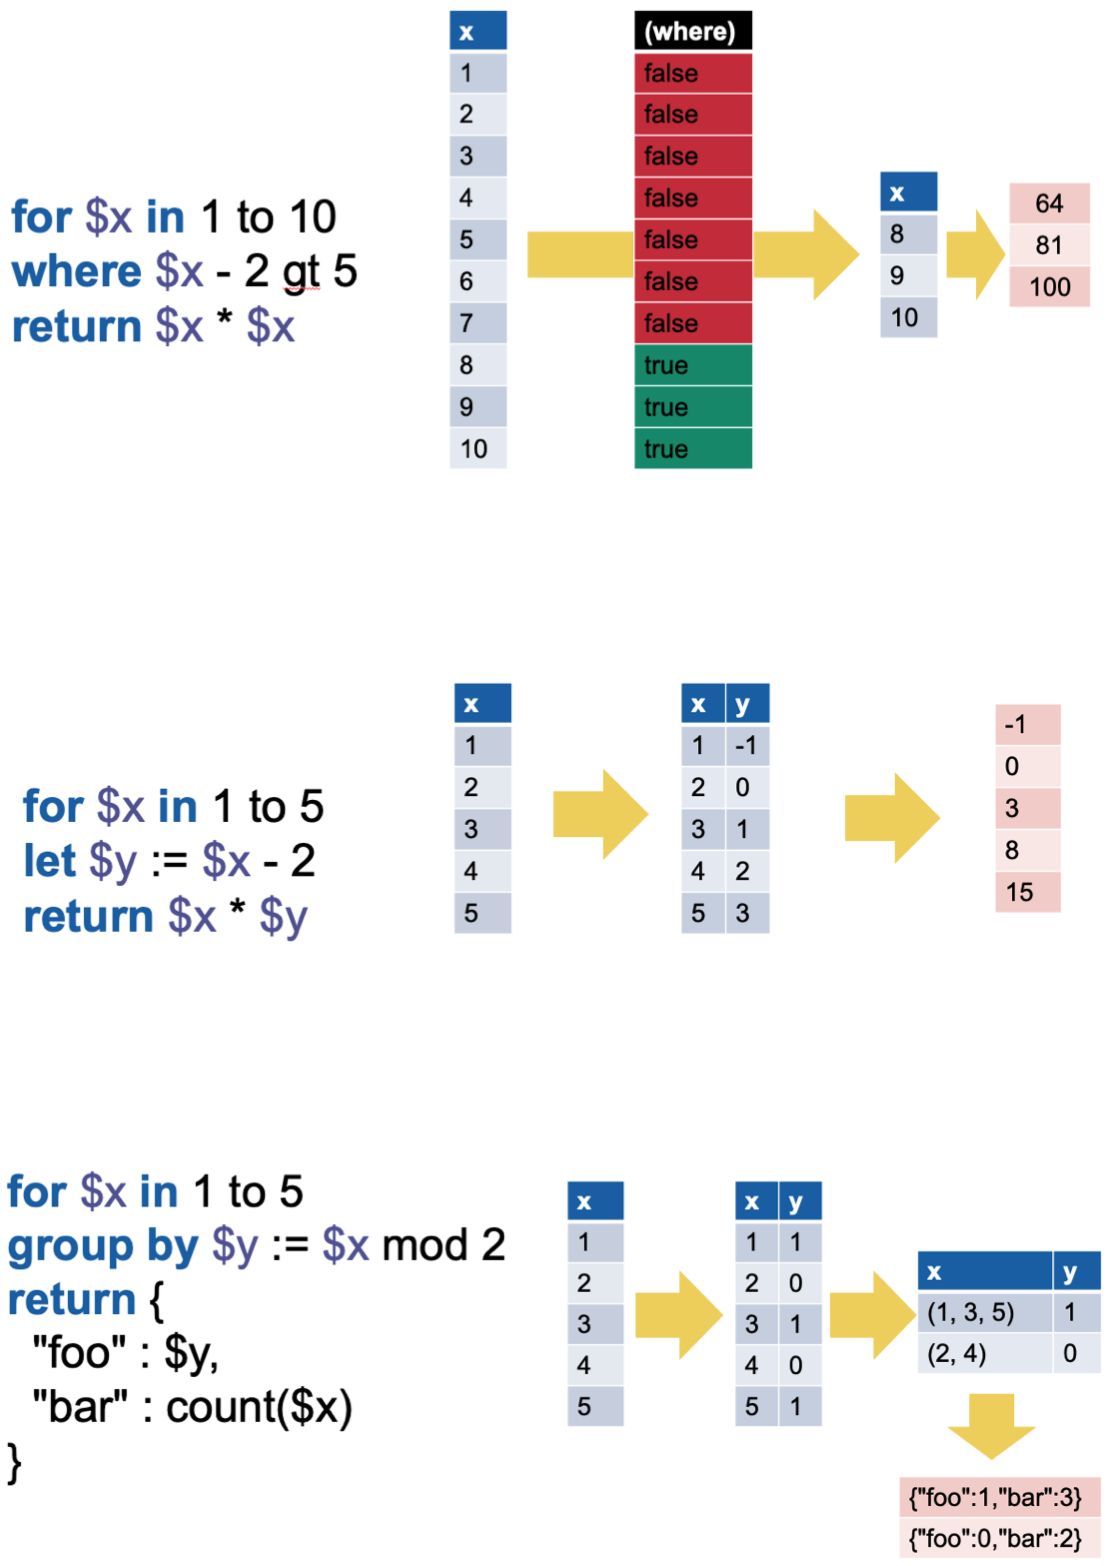
\includegraphics[width=0.5\textwidth]{Figures/TupleStream.png}
    \caption{Tuple Stream Vizualization}\label{fig:TupleStream}
\end{figure}


\subsubsection{Relational Algebra with JSONiq}
Assume we are dealing again with the following dataset:

\begin{lstlisting}[style=json]
// products.json
{"id":1, "type" : "tv", "store":1}
{"id":2, "type" : "tv", "store":2}
{"id":3, "type" : "phone", "store":2}
{"id":4, "type" : "tv", "store":3}
{"id":5, "type" : "teapot", "store":2}
{"id":6, "type" : "tv", "store":1}
{"id":7, "type" : "teapot", "store":2}
{"id":8, "type" : "phone", "store":4}

// stores.json
{ "id" : 1, "country" : "Switzerland" }
{ "id" : 2, "country" : "Germany" }
{ "id" : 3, "country" : "United States" }
\end{lstlisting}

\paragraph{Selection}
Example:
\begin{lstlisting}[style=json]
// Query:
for $p in json-file("products.json")
where $p.store = "1"
return $p
// Result:
{"id":1, "type" : "tv", "store":1}
{"id":6, "type" : "tv", "store":1}
\end{lstlisting}

\paragraph{Projection}
Example:
\begin{lstlisting}[style=json]
// Query:
for $p$ in json-file("products.json")
return project($p,("id","type"))
// Result:
{"id" : 1, "type" : "tv"}
{"id":2, "type" : "tv"}
{"id":3, "type" : "phone"}
...
\end{lstlisting}

\paragraph{Ordering}
Example:
\begin{lstlisting}[style=json]
// Query:
for $p$ in json-file("products.json")
order by $p.id
return $p
// Result:
{"id":1, "type" : "tv", "store":1}
{"id":2, "type" : "tv", "store":2}
{"id":3, "type" : "phone", "store":2}
...
\end{lstlisting}

\paragraph{Aggregation}
Example:
\begin{lstlisting}[style=json]
// Query:
for $p$ in json-file("products.json")
group by $t := $p.type
return {
    "type" : $t,
    "num" : count($p)
}
// Result:
{"type" : "tv", "num" : 4}
{"type" : "phone", "num" : 1}
{"type" : "teapot", "num" : 2}
\end{lstlisting}

\paragraph{Join}
RumbleDB auto-detects joins and it will implement it on top of Spark as actual joins.
Example:
\begin{lstlisting}[style=json]
// Query:
for $p in json-file("products.json")
for $s in json-file("stores.json")
where $p.store eq $s.id
return{
    "type" : $p.type,
    "country" : $s.country
}
// Result:
{"type" : "tv", "country" : "Switzerland"}
{"type" : "tv", "country" : "Germany"}
{"type" : "phone", "country" : "Germany"}
...
{"type" : "teapot", "country" : "Germany"}
\end{lstlisting}

\paragraph{Left-outer Join}
A special case of join where not everything has a match. You can implement that with the \texttt{allowing empty in} command. It will return \texttt{null} for empty items.
Example:
\begin{lstlisting}[style=json]
// Query:
for $p in json-file("products.json")
for $s allowing empty in
    json-file("store.json")[$p.store eq $$.id]
return {
    "type" : $p.type,
    "country" : $s.country
}
// Result:
{"type" : "tv", "country" : "Switzerland"}
{"type" : "tv", "country" : "Germany"}
...
{"type" : "teapot", "country" : "Germany"}
{"type" : "foo", "country" : null}
\end{lstlisting}

\paragraph{Denormalization}
This is something SQL cannot do. In the following example \texttt{\$\$} is the \textit{context item}. It is bound one-to-one to the items of the sequence it is refered to.

\begin{lstlisting}[style=json]
// Query:
for $s in json-file("stores.json")
let $p:= json-file("products.json")[$$.store eq $s.id]
return{
    "country" : $s.country,
    "products" : [$p.type]
}
// Result:
{"country" : "Switzerland", "products" : ["tv","tv"]}
{"country" : "Germany", "products" : ["tv","phone","teapot","teapot"]}
{"country" : "United States", "products" : ["tv"]}
\end{lstlisting}

\subsection{Types}

\subsubsection{Variable Types}
It is possible to annotate any FLWOR variable with an expected type as shown below.

\begin{lstlisting}[style=json]
let $path as string := "git-archive-big.json"
let $events as object* := json-file($path)
let $actors as object* := $events.actor
let $logins as string* := $actors.login
let $distinct-logins as string* := distinct-values($logins)
let $count as integer := count($distinct-logins)
return $count
\end{lstlisting}

Since every value in JSONiq is a sequence of item, a sequence type consists of two parts: an item type, and a cardinality.
Item types can be any of the builtin atomic types (JSound), as well as “object”, “array” and the most generic item type, “item”. Cardinality can be one of the following four:
\begin{itemize}
    \item Any number of items (suffix *), e.g. object*
    \item One or more items (suffix +), e.g. array+
    \item Zero or one item (suffix ?), e.g. boolean?
    \item Exactly one item (no suffix), e.g. integer
\end{itemize}
If it is detected, at runtime, that a sequence of items is bound to a variable but does not match the expected sequence type, either because one of the items does not match the expected item type, or because the cardinality of the sequence does not match the expected cardinality, then a type error is thrown and the query is not evaluated.
It is also possible to annotate variables in for clauses, however the cardinality of the sequence type of a for variable will logically be either one (no suffix), or zero-or-one (?) in the case that “allowing empty” is specified.

\subsubsection{Type Expressions}
JSONiq has a few expressions related to types.

An \texttt{instance of} expression checks whether a sequences matches a
sequence type, and returns true or false. This is similar to the homony- mous expression in Java.

\begin{lstlisting}[style=json]
// Query:
(3.14, "foo") instance of integer*,
([1], [ 2, 3 ]) instance of array+
// Result:
false
true  
\end{lstlisting}

A \texttt{cast as} expression casts single items to an expected item type.

\begin{lstlisting}[style=json]
// Query:
"3.14" cast as decimal
// Result:
3.14
\end{lstlisting}

A \texttt{castable as} expression tests whether a cast would succeed (in which case it returns true) or not (false).

\begin{lstlisting}[style=json]
// Query:
"3.14" castable as decimal
// Result:
true
\end{lstlisting}

A \texttt{treat as} expression checks whether its input sequence matches an expected type (like a type on a variable); if it does, the input sequence is returned unchanged. If not, an error is raised. This is useful in complex queries and for debugging purposes.

\begin{lstlisting}[style=json]
// Query:
[ 1, 2, 3, 4][] treat as integer+
// Result:
1
2
3
4
\end{lstlisting}

\subsubsection{Types in User-defined Functions}
JSONiq supports user-defined functions. Parameter types can be optionally specified, and a return type can also be optionally specified. The following two queries have the same result:

\begin{lstlisting}[style=json]
// Query 1:
declare function is-big-data(
    $threshold as integer,
    $objects as object*
) as boolean
{
    count($objects) gt $threshold
};

is-big-data(1000, json-file("git-archive.json"))

// Query 2:
declare function is-big-data(
    $threshold,
    $objects
)
{
    count($objects) gt $threshold
};

is-big-data(1000, json-file("git-archive.json"))

// Result:
true
\end{lstlisting}

\subsubsection{Validating against a schema}
It is possible to declare a schema, associating it with a user-defined type, and to validate a sequence of items against this user-defined type.

\begin{lstlisting}[style=json]
// Query:
declare type local:histogram as {
    "commits" : "short",
    "count" : "long"
};

validate type local:histogram* {
    for $event in json-file("git-archive-big.json")
    group by $nb-commits := (size($event.payload.commits), 0)[1]
    order by $nb-commits
    return {
        "commits" : $nb-commits,
        "count" : count($event)
    }
}

// Result:
{ "commits" : 0, "count" : 94554 }
{ "commits" : 1, "count" : 92094 }
{ "commits" : 2, "count" : 9951 }
{ "commits" : 3, "count" : 3211 }
{ "commits" : 4, "count" : 1525 }
...
\end{lstlisting}

If the results of a JSONiq query have been validated against a JSound schema, under specific conditions, then it is possible to save the output of the query in other formats than JSON, such as Parquet, Avro, or (if there is no nestedness) CSV. For that you would need to run this in Java (assume the above code is stored as query.jq):

\begin{lstlisting}[style=java]
java -jar rumbledb-1.19.0-standalone.jar run query.jq
    --output-path out
    --overwrite yes
    --number-of-output-partitions 1
    --output-format csv
    --output-foramt-option:header true
\end{lstlisting}

\subsection{Architecture of a Query Engine}
We now cover the physical architecture and implementation of a query engine such as RumbleDB.

\subsubsection{Static Phase}
When a query is received by an engine, it is text that needs to be parsed. The output of
this is a tree structure called an Abstract Syntax Tree.

An Abstract Syntax Tree, even though it already has the structure of a tree, is tightly tied to the original syntax. Thus, it needs to be converted into a more abstract Intermediate Representation called an expression tree. Every node in this tree corresponds to either an expression or a clause in the JSONiq language, making the design modular.

At this point, static typing takes place, meaning that the engine infers the static type of each expression, that is, the most specific type possible expected at runtime (but without actually running the pro- gram). User-specified types are also taken into account for this step. Inferring static types facilitates the optimization step.

Engines like RumbleDB perform their optimization round on this Intermediate Representation. Optimizations consist in changing the tree to another one that will evaluate faster, but without changing the semantics of the query (i.e., it should produce the same output).

Once optimizations have been done, RumbleDB decides the mode with which each expression and clause will be evaluated (locally, sequentially, in parallel, in DataFrames, etc). The resulting expression tree is then converted to a runtime iterator tree; this is the query plan that will actually be evaluated by the engine.

Every node in a runtime iterator tree outputs either a sequence of items (if it corresponds to an expression) or a tuple stream (if it corresponds to a clause other than the return clause).

\begin{figure}[h]
    \centering
    \includegraphics[width=\textwidth]{Figures/StaticPhase.png}
    \caption{Static Phase}
\end{figure}

\subsubsection{Dynamic Phase}
During the dynamic phase, the root of the tree is asked to produce a sequence of items, which is to be the final output of the query as a whole.

Then, recursively, each node in the tree will ask its children to produce sequences of items (or tuple streams). Each node then combines the sequences of items (or tuple streams) it receives from its children in order to produce its own sequence of items according to its semantics, and pass it to its parent. That way, the data flows all the way from the bottom of the tree to its root, and the final results are obtained and presented to the user or written to persistent storage (drive or data lake).

There are many different ways for a runtime iterator to produce an output sequence of items (or tuple stream) and pass it to its parent runtime iterator in the tree:

\begin{itemize}
    \item By materializing sequences of items (or tuple streams) completely in local computer memory.
    \item By locally iterating over each item in a sequence, one after the other (or over each tuple in a tuple stream, one after the other).
    \item By working in parallel over the sequence of items, internally stored as a Spark RDD.
    \item By working in parallel over the sequence fo items (or tuple stream), internally stored as a Spark DataFrame.
    \item By natively converting the semantics of the iterator to native Spark SQL.
\end{itemize}

\paragraph{Materialization}
When a sequence of items is materialized, it means that an actual List (or Array, or Vector), native to the language of implementation (in this case Java) is stored in local memory, filled with the items. This is, of course, only possible if the sequence is small enough that it fits.

The parent runtime iterator then directly processes this List in place, in order to produce its output.
A special case is when an expression is statically known to return either zero or one item (e.g., an addition, or a logical expression), but not more. Then no List structure is needed, and a single Item can be returned via a simple method call in the language of implementation (Java).

\paragraph{Streaming}
With larger sequences of items, it becomes impracticable to materialize because the footprint in memory becomes too large, and the size of the sequences that can be manipulated is strictly limited by the total memory available.

Thus, another technique is used instead: streaming. When a sequence of items (or tuple stream) is produced and consumed in a streaming fashion, it means that the items (or tuples) are produced and consumed one by one, iteratively. But the whole sequence of items (or tuple stream) is never stored anywhere.

With this technique, it is possible to process sequences that are much larger than memory, because the actual sequence is never fully stored. However, there are two problems with this: first, it can take a lot of time to go through the entire sequence (imagine doing so with billions or trillions of items). Second, there are expressions or clauses that are not compatible with streaming (consider, for example, the group by or order by clause, which cannot be implemented without materializing their full input).

\paragraph{Parallel Execution (with RDDs)}
When a sequence becomes unreasonably large, RumbleDB switches to a parallel execution, leveraging Spark capabilities: the sequences of items are passed and processed as RDDs of Item objects. Each runtime iterator then calls Spark transformations on these RDDs to produce an output RDD, or in some cases (e.g., count()) calls a Spark action to produce a single, local, materialized Item with an action.

A Spark transformation or action often needs to be supplied with an additional function (e.g., a map function, a filter function), called a Spark UDF (for “User-Defined Function”). What RumbleDB then does is that it squeezes an entire runtime iterator subtree into a UDF, so that this subtree can be recursively evaluated on each node of the cluster, as a local execution (materialized or streaming).

For example, imagine a filter expression, with a specific predicate, on a sequence of a billion items. If the input sequence is physically available as an RDD, RumbleDB squeezes the predicate's runtime iterator tree into a UDF, and invokes the filter() transformation with this UDF, resulting in a smaller RDD that contains the filtered sequence of items. Physically, the predicate's runtime iterator tree will be evalu- ated on items, in parallel, across thousands of machines in the cluster; relative to each one of these machines, this is a local execution (local to each machine), where the predicate iterator streams over each batch.

The use of RDDs is specific to sequences of items and does not exist for tuple streams.

\paragraph{Parallel execution (with DataFrames)}

The RDD implementation supports heterogeneous sequences by leveraging the polymorphism of Item objects. However, this is not efficient in the case that Items in the same sequence happen to have a regular structure.

Thus, if the Items in a sequence are valid against a specific schema, or even against an array type or an atomic type, the underlying physical storage in memory relies on Spark DataFrames instead of RDDs. Homogeneous sequences of arrays or of atomics (e.g., a sequence of in- tegers) are physical implemented as a one-column DataFrame with the corresponding type.

Thus, there exists a mapping from JSONiq types to Spark SQL types. In the case that there is no corresponding Spark SQL type, the implementation falls back to RDDs.

To summarize, homogeneous sequences of the most common types are stored in DataFrames, and RDDs are used in all other cases.

DataFrames are also consistently used for storing tuple streams and parallelizing the execution of FLWOR clauses. In FLWOR DataFrames, every column corresponds to one FLWOR variable, which is similar to the visuals provided earlier for FLWOR expressions in this chapter. The column type can either be native if the variable type can be mapped seamlessly to a Spark SQL type. Otherwise, the column type will be binary and Items are serialized to sequences of types and deserialized back on demand.


\paragraph{Parellel execution (with Native SQL)}

In some cases (more in every release), RumbleDB is able to evaluate the query using only Spark SQL, compiling JSONiq to SQL directly instead of packing Java runtime iterators in UDFs. This leads to faster execution, because UDFs are slower than a native execution in SQL. This is because, to a SQL optimizer, UDFs are opaque and prevent automatic optimizations.

RumbleDB switches seamless between all execution modes, even within the same query, as shown on the following diagram.


\begin{figure}[ht]
    \centering
    \includegraphics[width=\textwidth]{Figures/SQLExecution.png}
    \caption{Pipeline Parallel Execution with SQL}
\end{figure}





\end{document}